\chapter{Resultados y análisis}
\label{cap:resultados}

Resultados y análisis.

% En este capítulo se exponen los hallazgos empíricos y los resultados derivados de la aplicación secuencial de las fases del ciclo de vida de la metodología CRISP-DM. Inicialmente, se documentan las auditorías estructurales aplicadas sobre los registros brutos del sistema de Grupos Relacionados por el Diagnóstico (GRD). Posteriormente, se detallan los perfiles descriptivos obtenidos a partir del Análisis Exploratorio de Datos (EDA) y la jerarquización de factores críticos mediante los modelos de Inteligencia Artificial Explicable.

\section{Resultados de la exploración de datos (Fase 2)}
\label{sec:resultados_fase2}

\subsection{Resultados del análisis de los archivos brutos de GRD}

Durante la auditoría estructural sobre los archivos planos y anuales de GRD descargados desde la plataforma de datos abiertos, se obtuvo la siguiente codificación de caracteres para cada archivo, la presencia de anomalías de dimensionalidad en filas específicas (filas con más columnas que el resto) y modificaciones en las variables identificadoras de los pacientes. Estos resultados se resumen en la Tabla \ref{tab:auditoria_inicial_grd}:

\begin{table}[htbp]
\centering
\footnotesize
\setlength{\tabcolsep}{4pt}
\renewcommand{\arraystretch}{1.2}
\caption{Resultados de la auditoría técnica y estructural de los archivos brutos GRD (2019-2024).}
\label{tab:auditoria_inicial_grd}
\begin{tabular}{|c|c|c|c|l|}
\hline
\parbox[t]{1cm}{\textbf{Período}} & 
\parbox[t]{2.3cm}{\textbf{Tamaño físico\\(Bytes)}} & 
\parbox[t]{2.0cm}{\textbf{Codificación\\aprobada}} & 
\parbox[t]{2.5cm}{\textbf{Volumen Total\\(Filas / columnas)}} & 
\parbox[t]{5.2cm}{\textbf{Hallazgos y observaciones\\estructurales}} \\ \hline

\parbox[t]{1cm}{2019} & 
\parbox[t]{2.3cm}{572.538.020} & 
\parbox[t]{2.0cm}{\texttt{utf-8}} & 
\parbox[t]{2.5cm}{1.151.475 / 129} & 
\parbox[t]{5.2cm}{Estructura íntegra sin presencia de filas defectuosas. Preserva identificador histórico \texttt{CIP\_ENCRIPTADO}.} \\ \hline

\parbox[t]{1cm}{2020} & 
\parbox[t]{2.3cm}{397.026.707} & 
\parbox[t]{2.0cm}{\texttt{utf-8}} & 
\parbox[t]{2.5cm}{781.912 / 129} & 
\parbox[t]{5.2cm}{Disminución del volumen total debido probablemente al impacto sanitario pandémico. Hay consistencia del esquema de columnas.} \\ \hline

\parbox[t]{1cm}{2021} & 
\parbox[t]{2.3cm}{428.657.825} & 
\parbox[t]{2.0cm}{\texttt{utf-8-sig}} & 
\parbox[t]{2.5cm}{816.909 / 129} & 
\parbox[t]{5.2cm}{Inclusión programática de la marca de orden de bytes (BOM) al inicio del archivo. Hubo ingesta limpia sin pérdida.} \\ \hline

\parbox[t]{1cm}{2022} & 
\parbox[t]{2.3cm}{960.774.530} & 
\parbox[t]{2.0cm}{\texttt{utf-16}} & 
\parbox[t]{2.5cm}{932.840 / 129} & 
\parbox[t]{5.2cm}{Migración sistémica a codificación de 16 bits. Hubo una detección de una anomalía posicional (línea 120.127 con 130 columnas, en vez de 129), corregida en preprocesamiento.} \\ \hline

\parbox[t]{1cm}{2023} & 
\parbox[t]{2.3cm}{1.075.450.968} & 
\parbox[t]{2.0cm}{\texttt{utf-16}} & 
\parbox[t]{2.5cm}{1.039.587 / 129} & 
\parbox[t]{5.2cm}{Incremento del volumen de registros por sobre el millón de egresos. Obtuvo un esquema libre de problemas de delimitación.} \\ \hline

\parbox[t]{1cm}{2024} & 
\parbox[t]{2.3cm}{566.268.922} & 
\parbox[t]{2.0cm}{\texttt{latin1}} & 
\parbox[t]{2.5cm}{1.085.813 / 129} & 
\parbox[t]{5.2cm}{Error crítico del analizador heurístico de codificación (\texttt{hp-roman8}, con confianza 0.01). Estabilizado mediante decodificación manual \texttt{latin1}. Y hubo una modificación del identificador del paciente a \texttt{ID\_BENEFICIARIO} (en el resto de años se le asignaba la variable \texttt{CIP\_ENCRIPTADO}).} \\ \hline
\end{tabular}
\end{table}

El análisis comparativo determinó que todas las columnas mantuvieron una equivalencia funcional a lo largo de los 6 años analizados y no cambiaron sus nombres, con excepción del cambio nominal del identificador del paciente en 2024 (que cambió de \texttt{CIP\_ENCRIPTADO} a \texttt{ID\_BENEFICIARIO}). Esta inconsistencia fue mitigada en la etapa de clasificación oncológica para evitar la pérdida de continuidad en el análisis temporal. 

Cabe destacar que los años 2019 y 2024 presentaron mayor cantidad de episodios (filas) que en los años intermedios, por otro lado, en los años 2020 y 2021 se observó una disminución del volumen de registros, probablemente debido al impacto sanitario de la pandemia de COVID-19.


\subsection{Distribución oncológica y control de la cohorte}

Tras la el filtrado inicial y clasificación de diagnósticos, el proceso de limpieza y unificación permitió retener un total de $5.808.455$ episodios clínicos válidos. Al aplicar el algoritmo de clasificación basado en el Capítulo II de la CIE-10 (C00-C97), se detectaron $498.618$ episodios que presentaron al menos un diagnóstico oncológico activo durante su estadía hospitalaria, tanto en su diagnóstico principal (\texttt{DIAGNOSTICO1}) como secundario (\texttt{DIAGNOSTICO2-35}).

Respecto a los episodios oncológicos identificados, se observaron diferencias entre los motivos de ingreso directo (diagnóstico principal) y las comorbilidades oncológicas (diagnósticos secundarios). En específico, el análisis reveló que el 4,68\% de los episodios de ingreso tenían un diagnóstico oncológico principal ($272.093$ instancias), mientras que un 3,90\% presentaban cáncer como diagnóstico secundario ($226.525$ instancias). En su conjunto, la cohorte oncológica representó el 8,58\% de todos los egresos hospitalarios de la red pública en el período estudiado, conformando un grupo de control (\texttt{SIN\_CANCER}) masivo de $5.309.837$ episodios (91,42\%).

Como se ve en la tabla \ref{tab:distribucion_anual_cohorte}, en 2024 hubo un mayor número de episodios oncológicos respecto al resto de años, con un total de $55.111$ episodios con cáncer como diagnóstico principal y $44.042$ episodios con cáncer como diagnóstico secundario, representando a un 9,14\% de los episodios hospitalarios de ese año, alineandose con la tendencia de proyección del cáncer indicada en antecedentes. En contraste, el año 2020 presentó la menor cantidad de episodios oncológicos, con $35.294$ episodios con cáncer como diagnóstico principal y $29.632$ episodios con cáncer como diagnóstico secundario, representando a un 8,30\% de los episodios hospitalarios de ese año, probablemente debido al impacto sanitario de la pandemia de COVID-19.

\begin{table}[htbp]
\centering
\scriptsize
\setlength{\tabcolsep}{3pt}
\renewcommand{\arraystretch}{1.2}
\caption{Distribución anual de episodios hospitalarios: Cohorte oncológica versus grupo de control (2019-2024).}
\label{tab:distribucion_anual_cohorte}
\begin{tabular}{|c|c|c|c|c|c|c|c|}
\hline
\parbox[t]{1.5cm}{\centering\textbf{Período}} & 
\parbox[t]{1.8cm}{\centering\textbf{Cáncer\\Principal}} & 
\parbox[t]{1.5cm}{\centering\textbf{Proporción\\Principal}} & 
\parbox[t]{1.8cm}{\centering\textbf{Cáncer\\Secundario}} & 
\parbox[t]{1.5cm}{\centering\textbf{Proporción\\Secundario}} & 
\parbox[t]{2.0cm}{\centering\textbf{Sin Cáncer\\(Control)}} & 
\parbox[t]{1.5cm}{\centering\textbf{Proporción\\Sin cáncer}} & 
\parbox[t]{1.8cm}{\centering\textbf{Total de\\episodios}} \\ \hline

\parbox[t]{1.5cm}{\centering 2019} & \parbox[t]{1.8cm}{\raggedleft 46.241} & \parbox[t]{1.5cm}{\raggedleft 4,02\%} & \parbox[t]{1.8cm}{\raggedleft 51.588} & \parbox[t]{1.5cm}{\raggedleft 4,48\%} & \parbox[t]{2.0cm}{\raggedleft 1.053.569} & \parbox[t]{1.5cm}{\raggedleft 91,50\%} & \parbox[t]{1.8cm}{\raggedleft 1.151.398} \\ \hline
\parbox[t]{1.5cm}{\centering 2020} & \parbox[t]{1.8cm}{\raggedleft 35.294} & \parbox[t]{1.5cm}{\raggedleft 4,51\%} & \parbox[t]{1.8cm}{\raggedleft 29.632} & \parbox[t]{1.5cm}{\raggedleft 3,79\%} & \parbox[t]{2.0cm}{\raggedleft 716.985} & \parbox[t]{1.5cm}{\raggedleft 91,70\%} & \parbox[t]{1.8cm}{\raggedleft 781.911} \\ \hline
\parbox[t]{1.5cm}{\centering 2021} & \parbox[t]{1.8cm}{\raggedleft 38.836} & \parbox[t]{1.5cm}{\raggedleft 4,75\%} & \parbox[t]{1.8cm}{\raggedleft 29.090} & \parbox[t]{1.5cm}{\raggedleft 3,56\%} & \parbox[t]{2.0cm}{\raggedleft 748.983} & \parbox[t]{1.5cm}{\raggedleft 91,68\%} & \parbox[t]{1.8cm}{\raggedleft 816.909} \\ \hline
\parbox[t]{1.5cm}{\centering 2022} & \parbox[t]{1.8cm}{\raggedleft 44.827} & \parbox[t]{1.5cm}{\raggedleft 4,81\%} & \parbox[t]{1.8cm}{\raggedleft 33.242} & \parbox[t]{1.5cm}{\raggedleft 3,56\%} & \parbox[t]{2.0cm}{\raggedleft 854.768} & \parbox[t]{1.5cm}{\raggedleft 91,63\%} & \parbox[t]{1.8cm}{\raggedleft 932.837} \\ \hline
\parbox[t]{1.5cm}{\centering 2023} & \parbox[t]{1.8cm}{\raggedleft 51.784} & \parbox[t]{1.5cm}{\raggedleft 4,98\%} & \parbox[t]{1.8cm}{\raggedleft 38.931} & \parbox[t]{1.5cm}{\raggedleft 3,74\%} & \parbox[t]{2.0cm}{\raggedleft 948.872} & \parbox[t]{1.5cm}{\raggedleft 91,27\%} & \parbox[t]{1.8cm}{\raggedleft 1.039.587} \\ \hline
\parbox[t]{1.5cm}{\centering 2024} & \parbox[t]{1.8cm}{\raggedleft 55.111} & \parbox[t]{1.5cm}{\raggedleft 5,08\%} & \parbox[t]{1.8cm}{\raggedleft 44.042} & \parbox[t]{1.5cm}{\raggedleft 4,06\%} & \parbox[t]{2.0cm}{\raggedleft 986.660} & \parbox[t]{1.5cm}{\raggedleft 90,87\%} & \parbox[t]{1.8cm}{\raggedleft 1.085.813} \\ \hline
\rowcolor{gray!20}
\parbox[t]{1.5cm}{\centering\textbf{TOTAL GENERAL}} & \parbox[t]{1.8cm}{\raggedleft\textbf{272.093}} & \parbox[t]{1.5cm}{\raggedleft\textbf{4,68\%}} & \parbox[t]{1.8cm}{\raggedleft\textbf{226.525}} & \parbox[t]{1.5cm}{\raggedleft\textbf{3,90\%}} & \parbox[t]{2.0cm}{\raggedleft\textbf{5.309.837}} & \parbox[t]{1.5cm}{\raggedleft\textbf{91,42\%}} & \parbox[t]{1.8cm}{\raggedleft\textbf{5.808.455}} \\ \hline
\end{tabular}
\end{table}

Por otro lado, la Figura \ref{fig:proporcion_total} muestra la distribución de los diagnósticos oncológicos en la población general, demostrando que la mayoría de episodios oncológicos se presentaron como diagnóstico principal (4,68\%) en comparación con los diagnósticos secundarios (3,90\%). Esto sugiere que el cáncer es a menudo la razón primaria de hospitalización, aunque también es común que los pacientes ingresen por otras urgencias y tengan cáncer como comorbilidad. En conjunto, la cohorte oncológica representó el 8,58\% de todos los egresos hospitalarios, lo que resalta la significativa carga que el cáncer impone sobre el sistema de salud pública chileno. Además, como se tenía previsto, la mayor cantidad de episodios corresponden a pacientes sin diagnóstico oncológico (grupo de control, \texttt{SIN\_CANCER}), representando el 91,42\% de los episodios hospitalarios. Este grupo masivo de control es fundamental para evitar sesgos de selección y para permitir comparaciones robustas entre pacientes oncológicos y no oncológicos en las fases posteriores del análisis, especialmente al evaluar factores de riesgo asociados al cáncer.

\begin{figure}[htbp]
    \centering
	\captionsetup{justification=centering}
    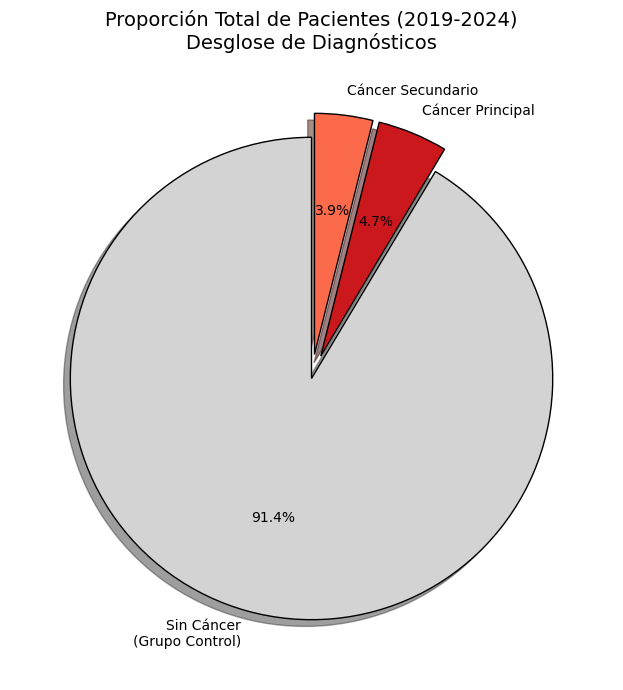
\includegraphics[width=0.6\textwidth]{images/proporcion_total_pacientes.png}
    \caption{Proporción total de pacientes y desglose de diagnósticos oncológicos (2019-2024).
    \\Fuente: Elaboraci\'on propia, 2026.}
    \label{fig:proporcion_total}
\end{figure}

Finalmente, se realizó un gráfico de barra para visualizar la distribución de cada tipo de cáncer según la codificación CIE-10 (Figura \ref{fig:barras_categorias}), en donde se observa que la mayoría de los episodios oncológicos se concentraron en cáncer de órganos digestivos (C15-C26) con $133.249$ episodios, seguidos por neoplasias de tejidos linfoide, hematopoyético y relacionados (C81-C96) con $85.492$ episodios, cáncer de mama (C50) con $59.990$ episodios y tumores en órganos genitales femeninos (C51-C58) con $42.030$ episodios.En donde, esta distribución confirma la alta demanda de recursos especializados que estas localizaciones específicas exigen dentro del sistema hospitalario chileno, lo que tiene implicaciones directas para la planificación de servicios oncológicos y la asignación de recursos.

\begin{figure}[htbp]
    \centering
	\captionsetup{justification=centering}
    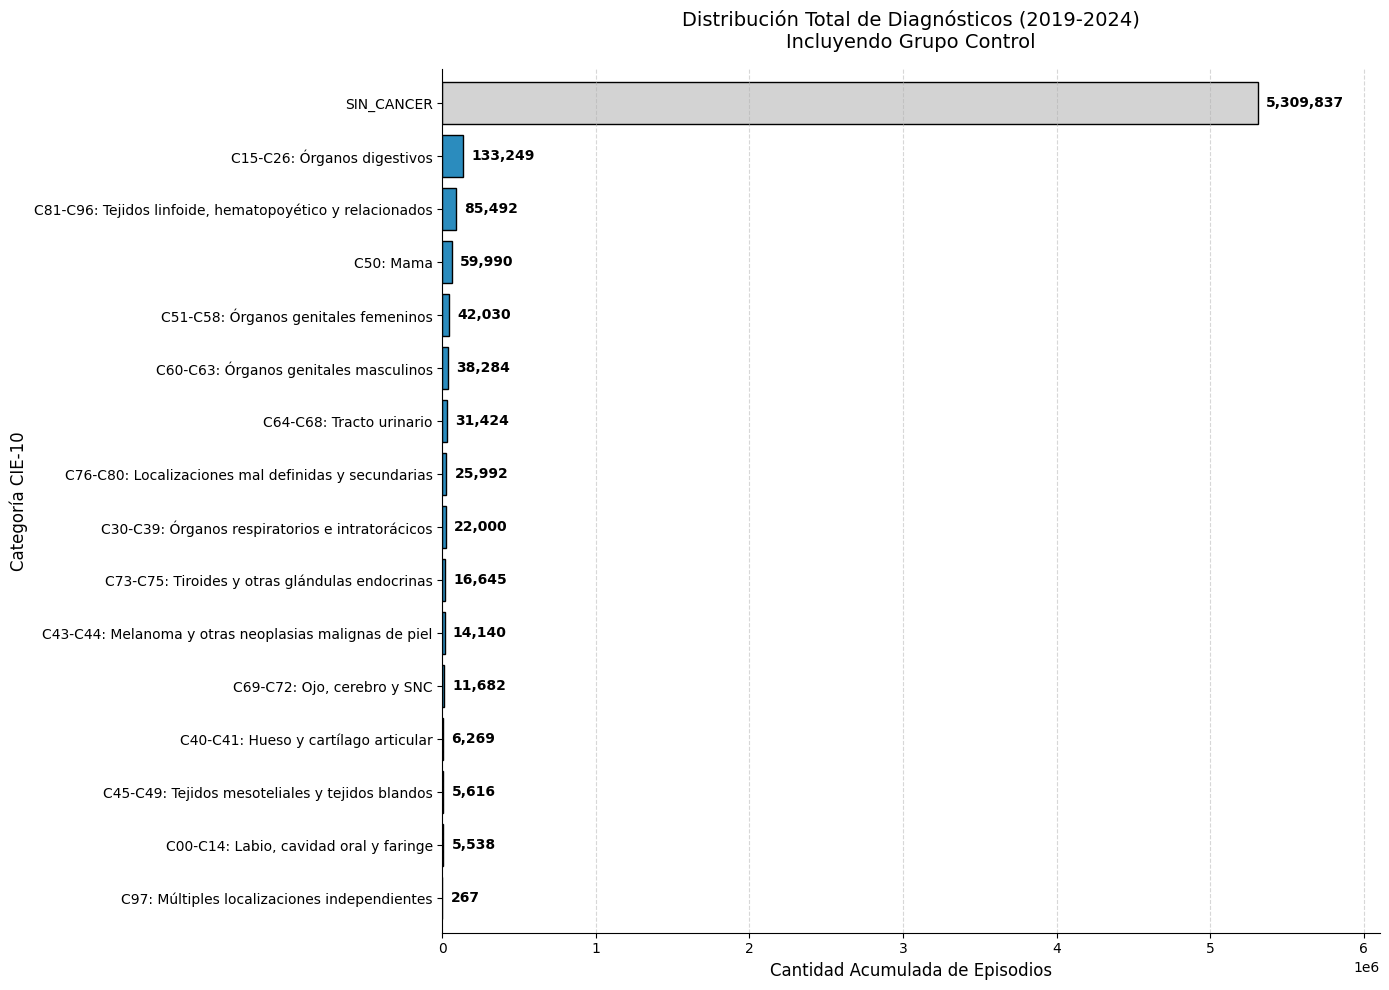
\includegraphics[width=1\textwidth]{images/barras_total_pacientes.png}
    \caption{Distribución de episodios según categoría CIE-10 frente al grupo de control.
    \\Fuente: Elaboraci\'on propia, 2026.}
    \label{fig:barras_categorias}
\end{figure}


\section{Análisis de variables demográficas, clínicas y hospitalarias}

\subsection{Análisis de variables identificadoras}

Para esta fase, se analizó la cardinalidad y distribución de cada variable identificadora presente en el registro hospitalario GRD, en donde la Tabla \ref{tab:cardinalidad_identificadores} expone el volumen de identificadores únicos para los pacientes, hospitales y médicos. En esta tabla se puede observar que todos los identificadores presentan un número alto de cardinalidad, en especial la cantidad de pacientes únicos (\texttt{CIP\_ENCRIPTADO}) que cuenta con más de 98.000 pacientes únicos en 2020. Por otro lado, hay entre 65 y 72 hospitales únicos durante el período analizado y más de 9.400 médicos únicos en cada año.

Respecto al análisis de reingresos de pacientes, registrados en la Tabla \ref{tab:reingresos_pacientes}, se observa que en los años 2019 y 2020, la frecuencia máxima es dominada de forma artificial por la etiqueta \texttt{SIN INFORMACIÓN}, registrando $8.307$ y $1.893$ episodios respectivamente, sin embargo, este hallazgo evidencia un defecto de la codificación de pacientes en la base de datos de origen, ya que el sistema agrupó por defecto bajo una misma cadena de texto (\texttt{SIN INFORMACIÓN}) a todos aquellos egresos hospitalarios cuyos datos de identificación civil no pudieron ser encriptados o resultaron ilegibles en el nodo central. Por otro lado, a partir del año 2021, se destacó el identificador anónimo \texttt{95162030}, el cual obtuvo la mayor cantidad de registros hospitalarios durante tres períodos consecutivos, registrando un mínimo de 294 reingresos en 2021 y un máximo de 523 episodios durante 2022. 

En relación a los hospitales, en la Tabla \ref{tab:concentracion_hospitales} se evidencia que, a pesar de que la cantidad de recintos hospitalarios creció de 65 (en 2019) a 72 (en 2024), la distribución de la carga asistencial fue marcadamente asimétrica. De forma consistente durante el periodo evaluado, los cinco recintos de mayor envergadura absorbieron entre el 16,5\% y el 18,6\% de la totalidad de los egresos hospitalarios de la red nacional, siendo el hospital codificado como \texttt{114101} el centro que lideró invariablemente este indicador de volumen asistencial (correspondiente al hospital Complejo Hospitalario Dr. Sótero del Río, de Santiago, Puente Alto).

Además del hospital \texttt{114101}, dentro de los recintos más frecuentes se encontraron los hospitales codificados como \texttt{106100} (Hospital Carlos Van Buren, Valparaíso), \texttt{118100} (Hospital Clínico Regional Dr. Guillermo Grant Benavente, Concepción), \texttt{109100} (Complejo Hospitalario San José, Santiago, Independencia), \texttt{121109} (Hospital Dr. Hernán Henríquez Aravena, Temuco), \texttt{113100} (Hospital Barros Luco Trudeau, Santiago, San Miguel), \texttt{116105} (Hospital Dr. César Garavagno Burotto, Talca), \texttt{120101} (Complejo Asistencial Dr. Víctor Ríos Ruiz, Los Ángeles) y \texttt{124105} (Hospital de Puerto Montt). Cabe mencionar que estas codificaciones están específicadas en las tablas maestras GRD obtenidas en el tablero de datos abiertos (\cite{fonasa_visor_grd}).

En base a las cardinalidades y frecuencias de cada identificador, se tomó la siguiente decisión para cada variable identificadora:
\begin{itemize}
    \item \textbf{Identificador de paciente (\texttt{CIP\_ENCRIPTADO} o \texttt{ID\_BENEFICIARIO}) (variable demográfica):} Se descartó su uso para la fase de modelado, ya que el código identificador encriptado de cada paciente no posee relación clínica ni operativa con su criticidad. Ya que se registró la existencia de pacientes con volúmenes de ingreso sospechosos o humanamente imposibles (como 8.307 episodios en 2019 para el registro \texttt{SIN INFORMACIÓN}, o 523 episodios para el ID \texttt{95162030} en 2022). Esto demuestra que la variable está probablemente contaminada con identificadores o códigos institucionales por defecto para pacientes sin registro, por lo cual, si se aplica transformaciones como One-Hot Encoding a una variable con miles de categorías crearía un conjunto de datos propenso al sobreajuste (\textit{overfitting}), afectando el rendimiento de los selectores de característica, además, cada episodio será evaluado como una instancia independiente según su contexto clínico. 
    \item \textbf{Identificador de hospital (\texttt{COD\_HOSPITAL}) (variable hospitalaria):} Se descartó su uso para la fase de modelado, ya que tiene una dimensionalidad muy alta, al tener entre 65 y 72 categorías distintas por año. Además, esta variable está anidada jerárquicamente dentro de la variable \texttt{SERVICIO\_SALUD} (que agrupa por macrozonas geográficas y tiene menor cardinalidad), entonces mantener ambas variables generaría colinealidad. Además, el propósito central de este estudio es apoyar la planificación sanitaria y gestión de recursos a nivel macro (redes de salud), dirigidos a instituciones como FONASA y MINSAL, por lo que el análisis a nivel de hospital individual escapa al alcance epidemiológico de la caracterización.
    \item \textbf{Identificador del médico de la primera intervención (\texttt{MEDICOINTERV1\_ENCRIPTADO}) (variable hospitalaria):} Se descartó su uso para la fase de modelado, ya que registra hasta 11.164 valores únicos por año, lo que generaría una matriz dispersa que penalizaría a los algoritmos de selección de características, por lo que el uso de este identificador es inviable metodológicamente. Además, el objetivo de este estudio es caracterizar, por ejemplo, qué procedimientos se hicieron, no quién los hizo.
    \item \textbf{Identificador del médico de alta (\texttt{MEDICOALTA\_ENCRIPTADO}) (variable hospitalaria):} Se descartó su uso para la fase de modelado, ya que registra una cardinalidad extrema de hasta 17.743 valores únicos por año, lo que generaría una matriz dispersa que penalizaría a los algoritmos de selección de características, por lo que el uso de este identificador es inviable metodológicamente. En otras palabras, transformar esta variable es computacionalmente ineficiente y desviaría al modelo de su objetivo principal, el cual es descubrir perfiles clínicos, demográficos y hospitalarios a nivel de red hospitalaria.
\end{itemize}

% Por otro lado, la Tabla \ref{tab:concentracion_hospitales} evidencia que, a pesar de que la cantidad de recintos hospitalarios emisores de datos GRD creció de 65 (en 2019) a 72 (en 2024), la distribución de la carga asistencial fue marcadamente asimétrica. De forma consistente durante el sexenio evaluado, los cinco recintos de mayor envergadura absorbieron entre el 16,5\% y el 18,6\% de la totalidad de los egresos hospitalarios de la red nacional, siendo el hospital codificado como \texttt{114101} el centro que lideró invariablemente este indicador de volumen asistencial.


% La existencia de un único código capaz de generar cientos de hospitalizaciones anuales dentro de una cohorte oncológica confirma que ciertos subgrupos de pacientes experimentan trayectorias asistenciales hiper-fragmentadas (como tratamientos seriados de quimioterapia, complicaciones agudas sucesivas o cuidados paliativos recurrentes). Este fenómeno valida la decisión de diseño de ingeniería de características tomada en este estudio, consistente en tratar cada hospitalización como un ``episodio operativo discreto e independiente'', ya que intentar modelar estas instancias vinculadas de forma tradicional habría provocado que un puñado de pacientes crónicos monopolizara el aprendizaje de los algoritmos supervisados, destruyendo la capacidad del modelo para generalizar el riesgo en la población oncológica general.

\begin{table}[htbp]
\centering
\scriptsize
\setlength{\tabcolsep}{3pt}
\renewcommand{\arraystretch}{1.2}
\caption{Cardinalidad de variables identificadoras en el registro hospitalario GRD (2019-2024).}
\label{tab:cardinalidad_identificadores}
\begin{tabular}{|c|c|c|c|c|c|c|}
\hline
\parbox[t]{2.5cm}{\centering\textbf{Identificador}} & 
\parbox[t]{1.8cm}{\centering\textbf{2019}} & 
\parbox[t]{1.8cm}{\centering\textbf{2020}} & 
\parbox[t]{1.8cm}{\centering\textbf{2021}} & 
\parbox[t]{1.8cm}{\centering\textbf{2022}} & 
\parbox[t]{1.8cm}{\centering\textbf{2023}} & 
\parbox[t]{1.8cm}{\centering\textbf{2024}} \\ \hline

\parbox[t]{2.5cm}{\raggedright\texttt{CIP\_ENCRIPTADO}\\\textit{(Pacientes únicos repetidos)}} & \parbox[t]{1.8cm}{\raggedleft 165.128} & \parbox[t]{1.8cm}{\raggedleft 98.379} & \parbox[t]{1.8cm}{\raggedleft 108.689} & \parbox[t]{1.8cm}{\raggedleft 129.107} & \parbox[t]{1.8cm}{\raggedleft 151.694} & \parbox[t]{1.8cm}{\raggedleft 161.533} \\ \hline
\parbox[t]{2.5cm}{\raggedright\texttt{COD\_HOSPITAL}\\\textit{(Hospitales emisores)}} & \parbox[t]{1.8cm}{\raggedleft 65} & \parbox[t]{1.8cm}{\raggedleft 65} & \parbox[t]{1.8cm}{\raggedleft 65} & \parbox[t]{1.8cm}{\raggedleft 68} & \parbox[t]{1.8cm}{\raggedleft 72} & \parbox[t]{1.8cm}{\raggedleft 72} \\ \hline
\parbox[t]{2.5cm}{\raggedright\texttt{MEDICOINTERV1}\\\textit{(Médicos tratantes)}} & \parbox[t]{1.8cm}{\raggedleft 9.617} & \parbox[t]{1.8cm}{\raggedleft 10.388} & \parbox[t]{1.8cm}{\raggedleft 9.476} & \parbox[t]{1.8cm}{\raggedleft 10.198} & \parbox[t]{1.8cm}{\raggedleft 10.569} & \parbox[t]{1.8cm}{\raggedleft 11.164} \\ \hline
\parbox[t]{2.5cm}{\raggedright\texttt{MEDICOALTA}\\\textit{(Médicos de egreso)}} & \parbox[t]{1.8cm}{\raggedleft 14.104} & \parbox[t]{1.8cm}{\raggedleft 16.051} & \parbox[t]{1.8cm}{\raggedleft 15.500} & \parbox[t]{1.8cm}{\raggedleft 15.720} & \parbox[t]{1.8cm}{\raggedleft 16.479} & \parbox[t]{1.8cm}{\raggedleft 17.743} \\ \hline
\end{tabular}
\end{table}

\begin{table}[htbp]
\centering
\scriptsize
\setlength{\tabcolsep}{4pt}
\renewcommand{\arraystretch}{1.2}
\caption{Casos críticos de reingreso hospitalario: Identificadores con máxima frecuencia anual de episodios (2019-2024).}
\label{tab:reingresos_pacientes}
\begin{tabular}{|c|l|l|}
\hline
\parbox[t]{1.2cm}{\centering\textbf{Año}} & 
\parbox[t]{5cm}{\centering\textbf{Identificador del paciente (\texttt{CIP\_ENCRIPTADO})}} & 
\parbox[t]{3.5cm}{\centering\textbf{Frecuencia máxima (Episodios)}} \\ \hline

\parbox[t]{1.2cm}{\centering 2019} & \parbox[t]{5cm}{\centering SIN INFORMACIÓN} & \parbox[t]{3.5cm}{\raggedleft 8.307} \\ \hline
\parbox[t]{1.2cm}{\centering 2020} & \parbox[t]{5cm}{\centering SIN INFORMACIÓN} & \parbox[t]{3.5cm}{\raggedleft 1.893} \\ \hline
\parbox[t]{1.2cm}{\centering 2021} & \parbox[t]{5cm}{\centering 95162030} & \parbox[t]{3.5cm}{\raggedleft 294} \\ \hline
\parbox[t]{1.2cm}{\centering 2022} & \parbox[t]{5cm}{\centering 95162030} & \parbox[t]{3.5cm}{\raggedleft 523} \\ \hline
\parbox[t]{1.2cm}{\centering 2023} & \parbox[t]{5cm}{\centering 95162030} & \parbox[t]{3.5cm}{\raggedleft 341} \\ \hline
\parbox[t]{1.2cm}{\centering 2024} & \parbox[t]{5cm}{\centering 78492052} & \parbox[t]{3.5cm}{\raggedleft 140} \\ \hline
\end{tabular}
\end{table}

\begin{table}[htbp]
\centering
\scriptsize
\setlength{\tabcolsep}{4pt}
\renewcommand{\arraystretch}{1.4}
\caption{Concentración de episodios asistenciales en los 5 establecimientos de salud de mayor volumen (2019-2024).}
\label{tab:concentracion_hospitales}
\begin{tabular}{|c|c|c|c|}
\hline
\parbox[t]{1.2cm}{\centering\textbf{Año}} & 
\parbox[t]{6.5cm}{\centering\textbf{Top 5 Hospitales (Código: Episodios)}} & 
\parbox[t]{2.2cm}{\centering\textbf{Total episodios\\(Top 5)}} & 
\parbox[t]{2.2cm}{\centering\textbf{Porcentaje de concentración}} \\ \hline

\parbox[t]{1.2cm}{\centering 2019} & 
\parbox[t]{6.5cm}{\raggedright Códigos 114101 (55.726), 106100 (42.026), 118100 (40.134), 109100 (35.921), 121109 (35.091)} & 
\parbox[t]{2.2cm}{\raggedleft 208.898} & 
\parbox[t]{2.2cm}{\raggedleft 18,1\%} \\ \hline

\parbox[t]{1.2cm}{\centering 2020} & 
\parbox[t]{6.5cm}{\raggedright Códigos 114101 (37.040), 113100 (28.652), 116105 (25.321), 109100 (24.903), 118100 (24.660)} & 
\parbox[t]{2.2cm}{\raggedleft 140.576} & 
\parbox[t]{2.2cm}{\raggedleft 18,0\%} \\ \hline

\parbox[t]{1.2cm}{\centering 2021} & 
\parbox[t]{6.5cm}{\raggedright Códigos 114101 (44.842), 118100 (28.853), 113100 (27.955), 116105 (25.610), 109100 (24.947)} & 
\parbox[t]{2.2cm}{\raggedleft 152.207} & 
\parbox[t]{2.2cm}{\raggedleft 18,6\%} \\ \hline

\parbox[t]{1.2cm}{\centering 2022} & 
\parbox[t]{6.5cm}{\raggedright Códigos 114101 (47.426), 118100 (31.167), 116105 (30.292), 120101 (29.101), 109100 (28.275)} &
\parbox[t]{2.2cm}{\raggedleft 166.261} & 
\parbox[t]{2.2cm}{\raggedleft 17,8\%} \\ \hline

\parbox[t]{1.2cm}{\centering 2023} & 
\parbox[t]{6.5cm}{\raggedright Códigos 114101 (49.653), 118100 (34.144), 116105 (32.148), 120101 (31.251), 121109 (29.786)} & 
\parbox[t]{2.2cm}{\raggedleft 176.982} & 
\parbox[t]{2.2cm}{\raggedleft 17,0\%} \\ \hline

\parbox[t]{1.2cm}{\centering 2024} & 
\parbox[t]{6.5cm}{\raggedright Códigos 114101 (49.411), 118100 (35.148), 116105 (33.858), 120101 (30.527), 124105 (30.453)} & 
\parbox[t]{2.2cm}{\raggedleft 179.397} & 
\parbox[t]{2.2cm}{\raggedleft 16,5\%} \\ \hline
\end{tabular}
\end{table}

% \subsection{Análisis de cardinalidad y riesgo de fuga de datos (\textit{Data Leakage})}

% En la Tabla \ref{tab:cardinalidad_identificadores} se expone el volumen de identificadores únicos para los principales actores del proceso hospitalario (pacientes, hospitales y médicos). El análisis de los pacientes únicos (`CIP_ENCRIPTADO`) reveló una alta prevalencia de readmisiones en el sistema. A modo de ejemplo, se detectaron casos extremos donde un solo identificador acumuló más de 8.000 episodios en 2019, o pacientes con más de 500 readmisiones en 2022. Esta anomalía estadística obligó a establecer que, metodológicamente, la unidad de análisis de los modelos predictivos sería el "episodio clínico" y no el "paciente", evitando así que las trayectorias atípicas hiperfrecuentes sesgaran el aprendizaje algorítmico.

% Por otro lado, la Tabla \ref{tab:concentracion_hospitales} evidencia que, a pesar de que la cantidad de recintos hospitalarios emisores de datos GRD creció de 65 (en 2019) a 72 (en 2024), la distribución de la carga asistencial fue marcadamente asimétrica. De forma consistente durante el sexenio evaluado, los cinco recintos de mayor envergadura absorbieron entre el 16,5\% y el 18,6\% de la totalidad de los egresos hospitalarios de la red nacional, siendo el hospital codificado como \texttt{114101} el centro que lideró invariablemente este indicador de volumen asistencial.

% Finalmente, el análisis exploratorio determinó la exclusión definitiva de las variables identificadoras de los profesionales de la salud (`MEDICOINTERV1` y `MEDICOALTA`). Tal como se refleja en la Tabla \ref{tab:cardinalidad_identificadores}, la cardinalidad de estas columnas osciló anualmente entre los 9.400 y los 17.700 médicos únicos. Retener estas variables en el conjunto de datos de entrenamiento no solo habría introducido ruido estadístico producto de la alta dispersión, sino que habría generado un riesgo crítico de \textit{Data Leakage}, obligando a los algoritmos de IA a inferir el riesgo clínico de un paciente memorizando la identidad del especialista a cargo, distorsionando así la capacidad de generalización del modelo.


\subsection{Análisis de variables temporales}

El análisis de las variables de tipo fecha constituyó un paso crítico para evaluar la coherencia cronológica de los registros asistenciales y asegurar la correcta construcción posterior de atributos derivados (como la edad y los días de estancia hospitalaria). Los indicadores de formato, cantidad de valores nulos, registros inválidos y rangos temporales identificados se indican en la Tabla \ref{tab:auditoria_fechas_grd}. 

En esta auditoría se detectó que las fechas de nacimiento e ingreso  presentaron una tasa mínima de valores nulos (0\%), lo que demuestra que constituyen campos obligatorios validados por los sistemas informáticos hospitalarios de admisión de la red pública. Sin embargo, se confirmó una alteración en el formato de registro exclusivo para el año 2023, el cual adoptó el estándar \texttt{dd-mm-yyyy} frente al formato ISO \texttt{yyyy-mm-dd} utilizado de manera homogénea en el resto de los años. Por otra parte, las fechas de traslado exhibieron un volumen incremental de valores nulos que osciló entre el 82,77\% y el 99,98\%, esto sugiere que el traslado interno entre múltiples servicios especializados (como unidad de tratamiento intermedio (UTI), unidad de cuidados intesivos (UCI) o cirugía) es un reflejo directo de la inestabilidad o severidad del paciente, ocurriendo únicamente en una fracción minoritaria de los ingresos asistenciales, mientras que la gran mayoría de la población concentró su estadía en un único servicio base (por ende, la mayoría de fechas de traslado tienden a tener cerca de un 100\% de valores nulos).

Otro hallazgo crítico se asoció a la fecha de procedimiento, la cual presentó una gran tasa de valores nulos y registros corruptos que alcanzaron casi el total de episodios ($5.808.446$), coexistiendo con formatos irreconocibles fuera del año 2019. Por otro lado, respecto a la fecha de intervención, se detectó una gran tasa de valores nulos (49\% correspondientes a $2.873.826$ registros) y un volumen de registros inválidos de $19.684$ filas corruptas, con una distorsión temporal que se extendió de manera inconsistente hasta el año 2090, lo que evidencia errores sistemáticos de digitación por parte de los operadores de la red de salud al ingresar las fechas de las intervenciones en los sistemas locales.

Finalmente, se tomaron las siguientes decisiones para cada variable temporal:
\begin{itemize}
    \item \textbf{Fecha de nacimiento (\texttt{FECHA\_NACIMIENTO}) (variable demográfica) y fecha de Ingreso (\texttt{FECHA\_INGRESO}) (variable hospitalaria):} Estas variables se descartaron en su formato crudo, pero se destinaron para generar la variable derivada de edad al ingreso, ya que ambas presentan 0\% de valores nulos reales en toda la cohorte, y a pesar de detectarse un quiebre de formato sistémico de la fecha en 2023 (cambio de formato \texttt{yyyy-mm-dd} a \texttt{dd-mm-yyyy}), se puede resolver exitosamente mediante un parseo robusto para calcular la variable derivada. Además, aunque los algoritmos basados en árboles (como Random Forest y XGBoost) no procesan objetos de tipo fecha (\textit{datetime}) de forma nativa, la diferencia matemática entre ambas fechas puede generar un determinante demográfico de riesgo crítico en oncología, el cual correspondería a la edad del paciente al ingreso hospitalario. 
    \item \textbf{Fechas de traslado (\texttt{FECHATRASLADO1} hasta \texttt{FECHATRASLADO9}) (variables hospitalarias):} Se descartaron completamente al presentar un déficit de datos masivos, en otras palabras, estas fechas no aportan valor predictivo directo, ya que la primera fecha de traslado (\texttt{FECHATRASLADO1}) posee un 82,77\% de valores nulos, escalando rápidamente hasta más de un 99\% de valores nulos a partir de la cuarta fecha. Además, mantener las fechas crudas y nulas solo introduciría matrices vacías que no aportan a la capacidad de generalización de los modelos. Sin embargo, se usará más adelante una variable categórica alineada a las fechas de traslado (conocida como \texttt{SERVICIO\_TRASLADO}) para generar la variable derivada \texttt{CANTIDAD\_TRASLADOS}, la cual sí puede aportar valor predictivo al capturar la cantidad de traslados intrahospitalarios que experimentó cada episodio, lo que es un indicador directo de inestabilidad clínica.
    \item \textbf{Fecha de alta (\texttt{FECHAALTA}) (variable hospitalaria):} Se descartó su uso en formato crudo, pero se destinará para generar la variable derivada de días de estancia hospitalaria, ya que esta fecha no es un descriptor del perfil del paciente por sí sola, pero al calcular la diferencia entre \texttt{FECHAALTA} y \texttt{FECHA\_INGRESO}, se puede obtener la variable derivada de \texttt{DIAS\_ESTADIA}, la cual potencialmente es uno de los indicadores más influyentes en el consumo de recursos y severidad hospitalaria, siendo esencial para la caracterización de grupos oncológicos. Además, la calidad de las fechas de alta es excelente, con una tasa cercana de 0\% de nulos reales, sujeto al mismo quiebre de formato en 2023 que la fecha de ingreso, la cual también tiene un 0\% de valores nulos.
    \item \textbf{Fecha de procedimiento (\texttt{FECHAPROCEDIMIENTO1}) (variable hospitalaria):} Se descartó completamente para el modelado, ya que esta columna está vacía e inválida en todos los archivos anuales analizados (2019-2024), por lo que carece de cualquier utilidad matemática o analítica.
    \item \textbf{Fecha de intervención (\texttt{FECHAINTERV1}) (variable hospitalaria):} Se descartó completamente su uso, ya que poseen una gran tasa de nulos del 49\% (probablemente correspondiente al porcentaje de pacientes que no requirieron intervención quirúrgica) y además, poseen un alto nivel de corrupción al presentar outliers e inconsistencias lógicas severas, como registros del año 2090 en admisiones que ocurrieron en 2023 o fechas de intervención registradas como 1902 en 2022. Por ende, el alto nivel de corrupción y la baja densidad de esta columna introducirían ruido excesivo en los modelos.

\end{itemize}



%Un hallazgo crítico derivado de esta auditoría fue la invalidez estructural absoluta detectada en la característica \texttt{FECHAPROCEDIMIENTO1}. Esta variable presentó una tasa de nulos y registros corruptos de prácticamente el 100\% ($n=5.808.446$), coexistiendo con formatos irreconocibles fuera del año 2019. Esta degradación del dato impidió su utilización matemática y justificó su exclusión radical durante la fase de ingeniería de características. 
% De manera similar, la variable \texttt{FECHAINTERV1} exhibió deficiencias graves de completitud (49,48\% de valores ausentes) y acumuló el mayor volumen de registros inválidos del sistema con $19.684$ filas corruptas. El análisis de rango de esta columna reveló una distorsión temporal que se extendió de manera anacrónica hasta el año 2090. Este fenómeno evidencia errores sistemáticos de digitación por parte de los operadores de la red de salud al ingresar manualmente las fechas de las intervenciones quirúrgicas en los sistemas locales. 

% Los resultados de la auditoría temporal revelaron un comportamiento diferenciado entre los campos obligatorios del núcleo administrativo y las variables operativas secundarias. En primer lugar, tanto \texttt{FECHA\_NACIMIENTO} como \texttt{FECHA\_INGRESO} presentaron una tasa de valores ausentes de 0,00\%, lo que demuestra que constituyen campos mandatorios validados por los sistemas informáticos hospitalarios en el nodo de admisión de la red pública. Sin embargo, en concordancia con los hallazgos de bajo nivel descritos en el marco metodológico, se confirmó una alteración en el formato de registro exclusivo para el año 2023, el cual adoptó el estándar \texttt{dd-mm-yyyy} frente al formato ISO \texttt{yyyy-mm-dd} utilizado de manera homogénea en el resto de los años del sexenio.
% Por otra parte, las variables de traslados intrahospitalarios (\texttt{FECHATRASLADO1} a \texttt{FECHATRASLADO9}) exhibieron un volumen incremental de valores ausentes que osciló entre el 82,77\% y el 99,98\%. Lejos de representar un defecto de calidad, este comportamiento posee una estricta coherencia operativa y clínica: el traslado interno entre múltiples servicios especializados (como tránsitos sucesivos entre medicina interna, unidades de cuidados críticos u oncología médica) es un reflejo directo de la inestabilidad o severidad del paciente, ocurriendo únicamente en una fracción minoritaria de los ingresos asistenciales, mientras que la vasta mayoría de la población concentró su estadía en un único servicio base.

Es fundamental destacar que, la totalidad de las características analizadas (a excepción de \texttt{FECHAPROCEDIMIENTO1}) registraron un rango válido de meses estrictamente acotado entre 1 y 12, y un rango de días contenido entre 1 y 31. Lo que confirmó que la estructura granular de los datos temporales era matemáticamente válida, lo que legitimó el cálculo con exactitud de las variables derivadas como edad y días de estancia.

\begin{table}[htbp]
\centering
\scriptsize
\setlength{\tabcolsep}{3pt}
\renewcommand{\arraystretch}{1.1}
\caption{Auditoría de consistencia, formato y cobertura de variables temporales (2019-2024).}
\label{tab:auditoria_fechas_grd}
\begin{tabular}{|l|c|c|c|c|}
\hline
\parbox[t]{2.8cm}{\textbf{Variable temporal}} & 
\parbox[t]{3.6cm}{\centering\textbf{Formato detectado\\(Variación anual)}} & 
\parbox[t]{2.2cm}{\centering\textbf{Valores nulos}} & 
\parbox[t]{1.3cm}{\centering\textbf{Registros\\inválidos}} & 
\parbox[t]{1.8cm}{\centering\textbf{Rango de\\años}} \\ \hline

\parbox[t]{2.8cm}{\texttt{FECHA\_NACIMIENTO}} & \parbox[t]{3.6cm}{\centering \texttt{yyyy-mm-dd}} & \parbox[t]{2.2cm}{\raggedleft 0 (0,00\%)} & \parbox[t]{1.3cm}{\raggedleft 21} & \parbox[t]{1.8cm}{\centering 1900-2024} \\ \hline
\parbox[t]{2.8cm}{\texttt{FECHA\_INGRESO}} & \parbox[t]{3.6cm}{\centering \texttt{dd-mm-yyyy} (2023) / \texttt{yyyy-mm-dd}} & \parbox[t]{2.2cm}{\raggedleft 0 (0,00\%)} & \parbox[t]{1.3cm}{\raggedleft 70} & \parbox[t]{1.8cm}{\centering 2011-2024} \\ \hline
\parbox[t]{2.8cm}{\texttt{FECHATRASLADO1}} & \parbox[t]{3.6cm}{\centering \texttt{dd-mm-yyyy} (2023) / \texttt{yyyy-mm-dd}} & \parbox[t]{2.2cm}{\raggedleft 4.807.468 (82,77\%)} & \parbox[t]{1.3cm}{\raggedleft 18} & \parbox[t]{1.8cm}{\centering 2011-2024} \\ \hline
\parbox[t]{2.8cm}{\texttt{FECHATRASLADO2}} & \parbox[t]{3.6cm}{\centering \texttt{dd-mm-yyyy} (2023) / \texttt{yyyy-mm-dd}} & \parbox[t]{2.2cm}{\raggedleft 5.475.101 (94,26\%)} & \parbox[t]{1.3cm}{\raggedleft 9} & \parbox[t]{1.8cm}{\centering 2011-2024} \\ \hline
\parbox[t]{2.8cm}{\texttt{FECHATRASLADO3}} & \parbox[t]{3.6cm}{\centering \texttt{dd-mm-yyyy} (2023) / \texttt{yyyy-mm-dd}} & \parbox[t]{2.2cm}{\raggedleft 5.704.842 (98,22\%)} & \parbox[t]{1.3cm}{\raggedleft 1} & \parbox[t]{1.8cm}{\centering 2011-2024} \\ \hline
\parbox[t]{2.8cm}{\texttt{FECHATRASLADO4}} & \parbox[t]{3.6cm}{\centering \texttt{dd-mm-yyyy} (2023) / \texttt{yyyy-mm-dd}} & \parbox[t]{2.2cm}{\raggedleft 5.771.110 (99,36\%)} & \parbox[t]{1.3cm}{\raggedleft 1} & \parbox[t]{1.8cm}{\centering 2011-2024} \\ \hline
\parbox[t]{2.8cm}{\texttt{FECHATRASLADO5}} & \parbox[t]{3.6cm}{\centering \texttt{dd-mm-yyyy} (2023) / \texttt{yyyy-mm-dd}} & \parbox[t]{2.2cm}{\raggedleft 5.794.707 (99,76\%)} & \parbox[t]{1.3cm}{\raggedleft 0} & \parbox[t]{1.8cm}{\centering 2011-2024} \\ \hline
\parbox[t]{2.8cm}{\texttt{FECHATRASLADO6}} & \parbox[t]{3.6cm}{\centering \texttt{dd-mm-yyyy} (2023) / \texttt{yyyy-mm-dd}} & \parbox[t]{2.2cm}{\raggedleft 5.802.255 (99,89\%)} & \parbox[t]{1.3cm}{\raggedleft 0} & \parbox[t]{1.8cm}{\centering 2011-2024} \\ \hline
\parbox[t]{2.8cm}{\texttt{FECHATRASLADO7}} & \parbox[t]{3.6cm}{\centering \texttt{dd-mm-yyyy} (2023) / \texttt{yyyy-mm-dd}} & \parbox[t]{2.2cm}{\raggedleft 5.805.382 (99,95\%)} & \parbox[t]{1.3cm}{\raggedleft 0} & \parbox[t]{1.8cm}{\centering 2013-2024} \\ \hline
\parbox[t]{2.8cm}{\texttt{FECHATRASLADO8}} & \parbox[t]{3.6cm}{\centering \texttt{dd-mm-yyyy} (2023) / \texttt{yyyy-mm-dd}} & \parbox[t]{2.2cm}{\raggedleft 5.806.762 (99,97\%)} & \parbox[t]{1.3cm}{\raggedleft 0} & \parbox[t]{1.8cm}{\centering 2013-2024} \\ \hline
\parbox[t]{2.8cm}{\texttt{FECHATRASLADO9}} & \parbox[t]{3.6cm}{\centering \texttt{dd-mm-yyyy} (2023) / \texttt{yyyy-mm-dd}} & \parbox[t]{2.2cm}{\raggedleft 5.807.482 (99,98\%)} & \parbox[t]{1.3cm}{\raggedleft 0} & \parbox[t]{1.8cm}{\centering 2014-2024} \\ \hline
\parbox[t]{2.8cm}{\texttt{FECHAALTA}} & \parbox[t]{3.6cm}{\centering \texttt{dd-mm-yyyy} (2023) / \texttt{yyyy-mm-dd}} & \parbox[t]{2.2cm}{\raggedleft 18 (0,00\%)} & \parbox[t]{1.3cm}{\raggedleft 0} & \parbox[t]{1.8cm}{\centering 2019-2024} \\ \hline
\parbox[t]{2.8cm}{\texttt{FECHAPROCEDIMIENTO1}} & \parbox[t]{3.6cm}{\centering \texttt{yyyymmdd} (2019) / Desconocido} & \parbox[t]{2.2cm}{\raggedleft 5.808.446 (100,0\%)} & \parbox[t]{1.3cm}{\raggedleft 9} & \parbox[t]{1.8cm}{\centering Inválido} \\ \hline
\parbox[t]{2.8cm}{\texttt{FECHAINTERV1}} & \parbox[t]{3.6cm}{\centering \texttt{dd-mm-yyyy} (2023) / \texttt{yyyy-mm-dd}} & \parbox[t]{2.2cm}{\raggedleft 2.873.826 (49,48\%)} & \parbox[t]{1.3cm}{\raggedleft 19.684} & \parbox[t]{1.8cm}{\centering 1911-2090} \\ \hline
\end{tabular}
\end{table}

\subsection{Análisis de variables categóricas}

La caracterización de los episodios hospitalarios exige evaluar cómo se distribuyen las variables que los algoritmos de aprendizaje automático procesarán como atributos de entrada o variables objetivo (en el caso de la mortalidad y severidad). En este contexto, se realizó un análisis de frecuencia para cada variable categórica, con el objetivo de identificar la presencia de categorías mayoritarias o minoritarias que podrían influir en el rendimiento de los modelos predictivos y detectar posibles errores de codificación o grandes volúmenes de datos faltantes que podrían requerir estrategias de imputación o exclusión. Además, el análisis contrastó la distribución de las categorías a lo largo del período 2019--2024 tanto para la cohorte oncológica como para la cohorte control.

\subsubsection{Variables categóricas objetivo (targets)}

Dentro de las variables categóricas objetivo, se encuentran las variables de mortalidad hospitalaria (originalmente denominada \texttt{TIPOALTA}) y de severidad (originalmente denominada \texttt{IR\_29301\_SEVERIDAD}). 

En primer lugar, dentro de los datos GRD se encuentran dos variables que describen la \textbf{mortalidad} hospitalaria: \texttt{IR\_29301\_MORTALIDAD} y \texttt{TIPOALTA}. Sin embargo, la primera es un índice sintético calculado por el sistema de codificación de GRD, siendo redudante retenerlo para el modelado, ya que la variable \texttt{TIPOALTA} es un descriptor categórico directo de la condición de alta del paciente, el cual incluye una categoría específica para la muerte hospitalaria, es decir, es la variable objetivo real y definitiva del desenlace del paciente. De esta forma, se ponderarían los factores de riesgo desde las condiciones clínicas reales del paciente (mortalidad real), en lugar de generar perfiles a través de un índice de predicción o de riesgo calculado por el sistema de codificación. 

Como se mencionó, la variable \texttt{TIPOALTA} representa la verdad fundamental (Ground Truth) del desenlace clínico de cada paciente (mortalidad). En el análisis de frecuencias de la Tabla \ref{tab:frecuencia_tipo_alta}, se puede observar que la tasa de mortalidad de los pacientes oncológicos duplicó, y en ocasiones triplicó, la tasa de mortalidad de la cohorte control. En específico, para pacientes con cáncer la cantidad de episodios con desenlace de muerte hospitalaria osciló entre el 5,4\% y 6,9\%, mientras que para el grupo control latasa de mortalidad se mantuvo entre el 2,3\% y 3,7\%.

Es de particular interés destacar la tasa de desfunción durante la pandemia de COVID-19 en los años 2020 y 2021, donde la mortalidad oncológica alcanzó sus picos máximos históricos (6,9\% y 6,5\%, respectivamente), a pesar de que el volumen absoluto de decesos (4.462 y 4.423) fue menor que en años previos. Este fenómeno estadístico probablemente se deba a la contracción severa de ingresos hospitalarios durante la pandemia, lo que concentró las admisiones estrictamente en pacientes con neoplasias en estado crítico o terminal. Además, mientras que la mortalidad del grupo control regresó a sus valores de línea base pre pandémicos en 2022 y 2023 (2,6\% y 2,3\%, respectivamente), la mortalidad oncológica se mantuvo elevada por encima de 5,9\% hasta 2024, lo que coincide con las proyecciones de desfunciones para la población con cáncer. 

Cabe mencionar que, para los algoritmos de aprendizaje automático, la variable \texttt{TIPOALTA} en conjunto de sus 11 categorías (domicilio, fallecido, hospitalización domiciliaria, derivación de otro hospital del servicio, alta voluntaria, derivación de otro hospital de la red nacional, derivación a otros centros (cárcel), fuga del paciente, derivación institución privada (compra de servicios), derivación institución privada (voluntario), no identificada), se binarizará en una variable dicotómica (\texttt{MORTALIDAD}) con las clases \texttt{Fallecido} (1) y \texttt{Vivo} (0), donde esta clase agrupará los episodios con desenlace de alta voluntaria, domicilio, derivaciones, entre otros, exceptuando las categorías marginales sin información (no identificada y desconocido), las cuales serán eliminadas al tener una distribución cercana al 0\% (100 casos en total durante todos los años).

\begin{table}[htbp]
\centering
\scriptsize
\setlength{\tabcolsep}{3pt}
\renewcommand{\arraystretch}{1.2}
\caption{Distribución anual de la condición al egreso (Tipo de Alta, sin procesar): Cohorte oncológica vs. grupo control (2019-2024).}
\label{tab:frecuencia_tipo_alta}
\begin{tabular}{|l|c|c|c|c|c|c|c|}
\hline
\parbox[t]{3.0cm}{\textbf{Condición al Egreso\\(Tipo de Alta)}} & 
\parbox[t]{1.6cm}{\centering\textbf{Cohorte}} & 
\parbox[t]{1.6cm}{\centering\textbf{2019}} & 
\parbox[t]{1.6cm}{\centering\textbf{2020}} & 
\parbox[t]{1.6cm}{\centering\textbf{2021}} & 
\parbox[t]{1.6cm}{\centering\textbf{2022}} & 
\parbox[t]{1.6cm}{\centering\textbf{2023}} & 
\parbox[t]{1.6cm}{\centering\textbf{2024}} \\ \hline

% DOMICILIO
\parbox[t]{3.0cm}{\textbf{Domicilio}} 
& \parbox[t]{1.6cm}{\centering Oncológica} & \parbox[t]{1.6cm}{\raggedleft 88.008 (90,0\%)} & \parbox[t]{1.6cm}{\raggedleft 56.334 (86,8\%)} & \parbox[t]{1.6cm}{\raggedleft 58.867 (86,7\%)} & \parbox[t]{1.6cm}{\raggedleft 67.703 (86,7\%)} & \parbox[t]{1.6cm}{\raggedleft 78.385 (86,4\%)} & \parbox[t]{1.6cm}{\raggedleft 84.680 (85,4\%)} \\ 
\parbox[t]{3.0cm}{} 
& \parbox[t]{1.6cm}{\centering Control} & \parbox[t]{1.6cm}{\raggedleft 964.012 (91,5\%)} & \parbox[t]{1.6cm}{\raggedleft 638.565 (89,1\%)} & \parbox[t]{1.6cm}{\raggedleft 657.403 (87,8\%)} & \parbox[t]{1.6cm}{\raggedleft 770.531 (90,1\%)} & \parbox[t]{1.6cm}{\raggedleft 857.820 (90,4\%)} & \parbox[t]{1.6cm}{\raggedleft 883.172 (89,5\%)} \\ \hline

% FALLECIDO
\parbox[t]{3.0cm}{\textbf{Fallecido}} 
& \parbox[t]{1.6cm}{\centering Oncológica} & \parbox[t]{1.6cm}{\raggedleft 5.321 (5,4\%)} & \parbox[t]{1.6cm}{\raggedleft 4.462 (6,9\%)} & \parbox[t]{1.6cm}{\raggedleft 4.423 (6,5\%)} & \parbox[t]{1.6cm}{\raggedleft 4.850 (6,2\%)} & \parbox[t]{1.6cm}{\raggedleft 5.314 (5,9\%)} & \parbox[t]{1.6cm}{\raggedleft 6.009 (6,1\%)} \\ 
\parbox[t]{3.0cm}{} 
& \parbox[t]{1.6cm}{\centering Control} & \parbox[t]{1.6cm}{\raggedleft 24.263 (2,3\%)} & \parbox[t]{1.6cm}{\raggedleft 25.480 (3,6\%)} & \parbox[t]{1.6cm}{\raggedleft 27.542 (3,7\%)} & \parbox[t]{1.6cm}{\raggedleft 22.529 (2,6\%)} & \parbox[t]{1.6cm}{\raggedleft 19.822 (2,1\%)} & \parbox[t]{1.6cm}{\raggedleft 20.673 (2,1\%)} \\ \hline

% HOSPITALIZACION DOMICILIARIA
\parbox[t]{3.0cm}{\textbf{Hosp. Domiciliaria}} 
& \parbox[t]{1.6cm}{\centering Oncológica} & \parbox[t]{1.6cm}{\raggedleft 1.319 (1,3\%)} & \parbox[t]{1.6cm}{\raggedleft 1.471 (2,3\%)} & \parbox[t]{1.6cm}{\raggedleft 2.110 (3,1\%)} & \parbox[t]{1.6cm}{\raggedleft 2.741 (3,5\%)} & \parbox[t]{1.6cm}{\raggedleft 3.531 (3,9\%)} & \parbox[t]{1.6cm}{\raggedleft 4.473 (4,5\%)} \\ 
\parbox[t]{3.0cm}{} 
& \parbox[t]{1.6cm}{\centering Control} & \parbox[t]{1.6cm}{\raggedleft 11.668 (1,1\%)} & \parbox[t]{1.6cm}{\raggedleft 12.600 (1,8\%)} & \parbox[t]{1.6cm}{\raggedleft 20.293 (2,7\%)} & \parbox[t]{1.6cm}{\raggedleft 20.667 (2,4\%)} & \parbox[t]{1.6cm}{\raggedleft 25.767 (2,7\%)} & \parbox[t]{1.6cm}{\raggedleft 32.259 (3,3\%)} \\ \hline

% DERIVACION OTRO HOSPITAL DEL SERVICIO
\parbox[t]{3.0cm}{\textbf{Deriv. Hosp. Servicio}} 
& \parbox[t]{1.6cm}{\centering Oncológica} & \parbox[t]{1.6cm}{\raggedleft 1.631 (1,7\%)} & \parbox[t]{1.6cm}{\raggedleft 1.198 (1,8\%)} & \parbox[t]{1.6cm}{\raggedleft 1.069 (1,6\%)} & \parbox[t]{1.6cm}{\raggedleft 1.242 (1,6\%)} & \parbox[t]{1.6cm}{\raggedleft 1.671 (1,8\%)} & \parbox[t]{1.6cm}{\raggedleft 2.147 (2,2\%)} \\ 
\parbox[t]{3.0cm}{} 
& \parbox[t]{1.6cm}{\centering Control} & \parbox[t]{1.6cm}{\raggedleft 23.575 (2,2\%)} & \parbox[t]{1.6cm}{\raggedleft 16.641 (2,3\%)} & \parbox[t]{1.6cm}{\raggedleft 17.252 (2,3\%)} & \parbox[t]{1.6cm}{\raggedleft 15.246 (1,8\%)} & \parbox[t]{1.6cm}{\raggedleft 18.834 (2,0\%)} & \parbox[t]{1.6cm}{\raggedleft 22.776 (2,3\%)} \\ \hline

% ALTA VOLUNTARIA
\parbox[t]{3.0cm}{\textbf{Alta Voluntaria}} 
& \parbox[t]{1.6cm}{\centering Oncológica} & \parbox[t]{1.6cm}{\raggedleft 526 (0,5\%)} & \parbox[t]{1.6cm}{\raggedleft 498 (0,8\%)} & \parbox[t]{1.6cm}{\raggedleft 569 (0,8\%)} & \parbox[t]{1.6cm}{\raggedleft 646 (0,8\%)} & \parbox[t]{1.6cm}{\raggedleft 710 (0,8\%)} & \parbox[t]{1.6cm}{\raggedleft 652 (0,7\%)} \\ 
\parbox[t]{3.0cm}{} 
& \parbox[t]{1.6cm}{\centering Control} & \parbox[t]{1.6cm}{\raggedleft 9.437 (0,9\%)} & \parbox[t]{1.6cm}{\raggedleft 7.071 (1,0\%)} & \parbox[t]{1.6cm}{\raggedleft 8.490 (1,1\%)} & \parbox[t]{1.6cm}{\raggedleft 10.075 (1,2\%)} & \parbox[t]{1.6cm}{\raggedleft 9.607 (1,0\%)} & \parbox[t]{1.6cm}{\raggedleft 9.999 (1,0\%)} \\ \hline

% DERIVACION RED NACIONAL
\parbox[t]{3.0cm}{\textbf{Deriv. Red Nacional}} 
& \parbox[t]{1.6cm}{\centering Oncológica} & \parbox[t]{1.6cm}{\raggedleft 659 (0,7\%)} & \parbox[t]{1.6cm}{\raggedleft 584 (0,9\%)} & \parbox[t]{1.6cm}{\raggedleft 541 (0,8\%)} & \parbox[t]{1.6cm}{\raggedleft 560 (0,7\%)} & \parbox[t]{1.6cm}{\raggedleft 688 (0,8\%)} & \parbox[t]{1.6cm}{\raggedleft 755 (0,8\%)} \\ 
\parbox[t]{3.0cm}{} 
& \parbox[t]{1.6cm}{\centering Control} & \parbox[t]{1.6cm}{\raggedleft 7.756 (0,7\%)} & \parbox[t]{1.6cm}{\raggedleft 6.287 (0,9\%)} & \parbox[t]{1.6cm}{\raggedleft 6.653 (0,9\%)} & \parbox[t]{1.6cm}{\raggedleft 5.979 (0,7\%)} & \parbox[t]{1.6cm}{\raggedleft 6.784 (0,7\%)} & \parbox[t]{1.6cm}{\raggedleft 7.183 (0,7\%)} \\ \hline

% DERIVACION OTROS CENTROS
\parbox[t]{3.0cm}{\textbf{Deriv. Otros Centros (cárcel)}} 
& \parbox[t]{1.6cm}{\centering Oncológica} & \parbox[t]{1.6cm}{\raggedleft 76 (0,1\%)} & \parbox[t]{1.6cm}{\raggedleft 171 (0,3\%)} & \parbox[t]{1.6cm}{\raggedleft 135 (0,2\%)} & \parbox[t]{1.6cm}{\raggedleft 116 (0,1\%)} & \parbox[t]{1.6cm}{\raggedleft 143 (0,2\%)} & \parbox[t]{1.6cm}{\raggedleft 139 (0,1\%)} \\ 
\parbox[t]{3.0cm}{} 
& \parbox[t]{1.6cm}{\centering Control} & \parbox[t]{1.6cm}{\raggedleft 2.904 (0,3\%)} & \parbox[t]{1.6cm}{\raggedleft 4.225 (0,6\%)} & \parbox[t]{1.6cm}{\raggedleft 3.903 (0,5\%)} & \parbox[t]{1.6cm}{\raggedleft 3.269 (0,4\%)} & \parbox[t]{1.6cm}{\raggedleft 3.354 (0,4\%)} & \parbox[t]{1.6cm}{\raggedleft 3.606 (0,4\%)} \\ \hline

% DERIVACION PRIVADA (COMPRA)
\parbox[t]{3.0cm}{\textbf{Deriv. Inst. Privada\\(Compra Serv.)}} 
& \parbox[t]{1.6cm}{\centering Oncológica} & \parbox[t]{1.6cm}{\raggedleft 144 (0,1\%)} & \parbox[t]{1.6cm}{\raggedleft 97 (0,1\%)} & \parbox[t]{1.6cm}{\raggedleft 112 (0,2\%)} & \parbox[t]{1.6cm}{\raggedleft 91 (0,1\%)} & \parbox[t]{1.6cm}{\raggedleft 142 (0,2\%)} & \parbox[t]{1.6cm}{\raggedleft 167 (0,2\%)} \\ 
\parbox[t]{3.0cm}{} 
& \parbox[t]{1.6cm}{\centering Control} & \parbox[t]{1.6cm}{\raggedleft 4.267 (0,4\%)} & \parbox[t]{1.6cm}{\raggedleft 2.333 (0,3\%)} & \parbox[t]{1.6cm}{\raggedleft 3.576 (0,5\%)} & \parbox[t]{1.6cm}{\raggedleft 2.282 (0,3\%)} & \parbox[t]{1.6cm}{\raggedleft 2.744 (0,3\%)} & \parbox[t]{1.6cm}{\raggedleft 2.698 (0,3\%)} \\ \hline

% FUGA DEL PACIENTE
\parbox[t]{3.0cm}{\textbf{Fuga del Paciente}} 
& \parbox[t]{1.6cm}{\centering Oncológica} & \parbox[t]{1.6cm}{\raggedleft 75 (0,1\%)} & \parbox[t]{1.6cm}{\raggedleft 60 (0,1\%)} & \parbox[t]{1.6cm}{\raggedleft 49 (0,1\%)} & \parbox[t]{1.6cm}{\raggedleft 69 (0,1\%)} & \parbox[t]{1.6cm}{\raggedleft 77 (0,1\%)} & \parbox[t]{1.6cm}{\raggedleft 79 (0,1\%)} \\ 
\parbox[t]{3.0cm}{} 
& \parbox[t]{1.6cm}{\centering Control} & \parbox[t]{1.6cm}{\raggedleft 4.066 (0,4\%)} & \parbox[t]{1.6cm}{\raggedleft 2.659 (0,4\%)} & \parbox[t]{1.6cm}{\raggedleft 2.544 (0,3\%)} & \parbox[t]{1.6cm}{\raggedleft 3.115 (0,4\%)} & \parbox[t]{1.6cm}{\raggedleft 3.147 (0,3\%)} & \parbox[t]{1.6cm}{\raggedleft 3.220 (0,3\%)} \\ \hline

% DERIVACION PRIVADA (VOLUNTARIO)
\parbox[t]{3.0cm}{\textbf{Deriv. Inst. Privada\\(Voluntario)}} 
& \parbox[t]{1.6cm}{\centering Oncológica} & \parbox[t]{1.6cm}{\raggedleft 65 (0,1\%)} & \parbox[t]{1.6cm}{\raggedleft 50 (0,1\%)} & \parbox[t]{1.6cm}{\raggedleft 51 (0,1\%)} & \parbox[t]{1.6cm}{\raggedleft 51 (0,1\%)} & \parbox[t]{1.6cm}{\raggedleft 54 (0,1\%)} & \parbox[t]{1.6cm}{\raggedleft 52 (0,1\%)} \\ 
\parbox[t]{3.0cm}{} 
& \parbox[t]{1.6cm}{\centering Control} & \parbox[t]{1.6cm}{\raggedleft 1.549 (0,1\%)} & \parbox[t]{1.6cm}{\raggedleft 1.102 (0,2\%)} & \parbox[t]{1.6cm}{\raggedleft 1.327 (0,2\%)} & \parbox[t]{1.6cm}{\raggedleft 1.075 (0,1\%)} & \parbox[t]{1.6cm}{\raggedleft 993 (0,1\%)} & \parbox[t]{1.6cm}{\raggedleft 1.074 (0,1\%)} \\ \hline
\end{tabular}
\end{table}

En segundo lugar, la variable de \textbf{severidad} hospitalaria (\texttt{IR\_29301\_SEVERIDAD}) es calculada por el agrupador IR-GRD a partir del diagnóstico principal, diagnósticos secundarios, procedimientos y características clínicas del episodio, expresándose en 4 niveles ordinales: 0 (sin gravedad), 1 (menor), 2 (moderada) y 3 (mayor).

Como se puede observar en la Tabla \ref{tab:frecuencia_severidad}, esta variable contiene una cardinalidad baja de 4 categorías, además, posee una distribución de valores nulos y desconocidos cercana al 0\% (89 casos en total entre todos los años), lo que la convierte en una variable objetivo de alta calidad para el modelado, por lo cual se decidió retener como variable ordinal sin necesidad de binarizarla ni transformarla. 

Especificamente, en el análisis de frecuencias se puede observar que, mientras que en la cohorte de control la mayor proporción de ingresos recae históricamente sobre la severidad menor de nivel 1 (alcanzando hasta un 50,5\% en 2019), el paciente oncológico demanda niveles de complejidad clínica más elevados, con una mayor proporción de ingresos en los niveles de severidad moderada (nivel 2) y mayor (nivel 3), alcanzando hasta un 31,4\% y 20,2\% respectivamente en 2019. En otras palabras, los datos evidencian que los episodios de cáncer están fuertemente dirigidos hacia la derecha de la escala de severidad clínica, ya que la severidad de nivel 2 (moderada) actúa como la moda estadística de esta cohorte.

Respecto al comportamiento de la severidad mayor (nivel 3) en la cohorte oncológica, se puede observar que, sufrió una escalada crítica a partir de 2020, saltando de un 20,2\% en 2019 a representar casi un tercio de las hospitalizaciones (30,5\%) al cierre de 2024. Este desplazamiento progresivo hacia los estratos de mayor gravedad podría indicar que las camas de la red oncológica están siendo ocupadas por pacientes con cuadros clínicos cada vez más deteriorados.

\begin{table}[htbp]
\centering
\scriptsize
\setlength{\tabcolsep}{3pt}
\renewcommand{\arraystretch}{1.2}
\caption{Distribución porcentual de los niveles de severidad: Cohorte oncológica vs. grupo control (2019-2024).}
\label{tab:frecuencia_severidad}
\begin{tabular}{|l|c|c|c|c|c|c|c|}
\hline
\parbox[t]{2.5cm}{\textbf{Nivel de Severidad}} & 
\parbox[t]{1.6cm}{\centering\textbf{Cohorte}} & 
\parbox[t]{1.6cm}{\centering\textbf{2019}} & 
\parbox[t]{1.6cm}{\centering\textbf{2020}} & 
\parbox[t]{1.6cm}{\centering\textbf{2021}} & 
\parbox[t]{1.6cm}{\centering\textbf{2022}} & 
\parbox[t]{1.6cm}{\centering\textbf{2023}} & 
\parbox[t]{1.6cm}{\centering\textbf{2024}} \\ \hline

% NIVEL 0
\parbox[t]{2.5cm}{\textbf{Nivel 0 (Sin gravedad)}} 
& \parbox[t]{1.6cm}{\centering Oncológica} & \parbox[t]{1.6cm}{\raggedleft 20.675 (21,1\%)} & \parbox[t]{1.6cm}{\raggedleft 3.648 (5,6\%)} & \parbox[t]{1.6cm}{\raggedleft 5.689 (8,4\%)} & \parbox[t]{1.6cm}{\raggedleft 7.909 (10,1\%)} & \parbox[t]{1.6cm}{\raggedleft 10.215 (11,3\%)} & \parbox[t]{1.6cm}{\raggedleft 11.081 (11,2\%)} \\ 
\parbox[t]{2.5cm}{} 
& \parbox[t]{1.6cm}{\centering Control} & \parbox[t]{1.6cm}{\raggedleft 181.842 (17,3\%)} & \parbox[t]{1.6cm}{\raggedleft 76.016 (10,6\%)} & \parbox[t]{1.6cm}{\raggedleft 97.249 (13,0\%)} & \parbox[t]{1.6cm}{\raggedleft 146.863 (17,2\%)} & \parbox[t]{1.6cm}{\raggedleft 183.335 (19,3\%)} & \parbox[t]{1.6cm}{\raggedleft 200.970 (20,4\%)} \\ \hline

% NIVEL 1
\parbox[t]{2.5cm}{\textbf{Nivel 1 (Menor)}} 
& \parbox[t]{1.6cm}{\centering Oncológica} & \parbox[t]{1.6cm}{\raggedleft 26.703 (27,3\%)} & \parbox[t]{1.6cm}{\raggedleft 19.058 (29,4\%)} & \parbox[t]{1.6cm}{\raggedleft 19.126 (28,2\%)} & \parbox[t]{1.6cm}{\raggedleft 20.488 (26,2\%)} & \parbox[t]{1.6cm}{\raggedleft 21.770 (24,0\%)} & \parbox[t]{1.6cm}{\raggedleft 23.198 (23,4\%)} \\ 
\parbox[t]{2.5cm}{} 
& \parbox[t]{1.6cm}{\centering Control} & \parbox[t]{1.6cm}{\raggedleft 531.868 (50,5\%)} & \parbox[t]{1.6cm}{\raggedleft 347.235 (48,4\%)} & \parbox[t]{1.6cm}{\raggedleft 321.010 (42,9\%)} & \parbox[t]{1.6cm}{\raggedleft 352.952 (41,3\%)} & \parbox[t]{1.6cm}{\raggedleft 366.924 (38,7\%)} & \parbox[t]{1.6cm}{\raggedleft 364.060 (36,9\%)} \\ \hline

% NIVEL 2
\parbox[t]{2.5cm}{\textbf{Nivel 2 (Moderada)}} 
& \parbox[t]{1.6cm}{\centering Oncológica} & \parbox[t]{1.6cm}{\raggedleft 30.680 (31,4\%)} & \parbox[t]{1.6cm}{\raggedleft 23.807 (36,7\%)} & \parbox[t]{1.6cm}{\raggedleft 23.718 (34,9\%)} & \parbox[t]{1.6cm}{\raggedleft 26.710 (34,2\%)} & \parbox[t]{1.6cm}{\raggedleft 31.917 (35,2\%)} & \parbox[t]{1.6cm}{\raggedleft 34.607 (34,9\%)} \\ 
\parbox[t]{2.5cm}{} 
& \parbox[t]{1.6cm}{\centering Control} & \parbox[t]{1.6cm}{\raggedleft 211.611 (20,1\%)} & \parbox[t]{1.6cm}{\raggedleft 152.747 (21,3\%)} & \parbox[t]{1.6cm}{\raggedleft 160.104 (21,4\%)} & \parbox[t]{1.6cm}{\raggedleft 186.550 (21,8\%)} & \parbox[t]{1.6cm}{\raggedleft 221.169 (23,3\%)} & \parbox[t]{1.6cm}{\raggedleft 234.258 (23,7\%)} \\ \hline

% NIVEL 3
\parbox[t]{2.5cm}{\textbf{Nivel 3 (Mayor)}} 
& \parbox[t]{1.6cm}{\centering Oncológica} & \parbox[t]{1.6cm}{\raggedleft 19.771 (20,2\%)} & \parbox[t]{1.6cm}{\raggedleft 18.413 (28,4\%)} & \parbox[t]{1.6cm}{\raggedleft 19.393 (28,6\%)} & \parbox[t]{1.6cm}{\raggedleft 22.960 (29,4\%)} & \parbox[t]{1.6cm}{\raggedleft 26.813 (29,6\%)} & \parbox[t]{1.6cm}{\raggedleft 30.265 (30,5\%)} \\ 
\parbox[t]{2.5cm}{} 
& \parbox[t]{1.6cm}{\centering Control} & \parbox[t]{1.6cm}{\raggedleft 128.227 (12,2\%)} & \parbox[t]{1.6cm}{\raggedleft 140.987 (19,7\%)} & \parbox[t]{1.6cm}{\raggedleft 170.620 (22,8\%)} & \parbox[t]{1.6cm}{\raggedleft 168.382 (19,7\%)} & \parbox[t]{1.6cm}{\raggedleft 177.414 (18,7\%)} & \parbox[t]{1.6cm}{\raggedleft 187.359 (19,0\%)} \\ \hline

\end{tabular}
\end{table}

\subsubsection{Variables categóricas de entrada}

A continuación, se presenta una lista de las variables categóricas de entrada provenientes de los datos GRD, en donde en base a su cardinalidad y tasa de frecuencias, se justificó su uso, agrupación o descarte para el modelado de desenlaces de riesgo de mortalidad, severidad y consumo de recursos:

\begin{enumerate}
    \item \textbf{Sexo:} Esta variable se decidió retenerla sin necesidad de transformarla, al presentar una cardinalidad perfecta de 2 categorías (Hombre y Mujer), tener una distribución equilibrada y constante a lo largo de los 6 años (entre 59\% mujeres y 41\% de hombres en la población general y entre 53\% de mujeres y 46\% de hombres en la cohorte oncológica), contener una tasa de valores desconocidos cercana al 0\% (559 casos en total durante todos los años), y además, ser un factor demográfico fundamental en la literatura médica para explicar la severidad de ciertos perfiles clínicos.
    \item \textbf{Etnia:} Esta variable se decidió transformar y binarizar en una variable que indique si la persona pertenece a un pueblo originario o no (\texttt{ES\_PUEBLO\_ORIGINARIO}), ya que la variable tiene 12 categorías (NINGUNO, OTRO, MAPUCHE, AYMARA, PASCUENSE, DIAGUITA, KAWESQAR, QUECHUA, YAGAN, COLLA, LICAN ANTAI, NO RESPONDE), y en ambas cohortes la mayoría de registros pertenecen a personas de ninguna etnia (entre 97\% y 98\% de casos), mientras dentro de las categorías de etnia, la más frecuente es la mapuche (entre 1,6\% y 1,9\% para la cohorte total, y entre 1,3\% y 1.9\% para la oncológica) y para el resto (como aymara y pascuense) las frecuencias bajan del 0,2\% a casi 0\%. Cabe mencionar que, las categorías NINGUNO y OTRO pertenecerían a la clase de personas que no pertenecen a un pueblo originario (0), ya que en los años 2022 y 2023 la categoría NINGUNO fue reemplazada por OTRO, mientras que el resto de categorías conformarían la clase positiva (1), excluyendo los valores nulos y los registros de NO RESPONDE, que en total registran 20 episodios durante los 6 años, lo que representa una tasa cercana al 0\%.
    \item \textbf{Provincia:} Esta variable se decidió retener y agrupar a nivel regional, ya que cuenta con 57 categorías provinciales, lo que generaría una matriz excesivamente dispersa al procesarla con One-Hot Encoding. Sin embargo, el dato geográfico es valioso, por ende, se plantea mapear y agrupar las 57 provincias en las 16 regiones de Chile (desde Arica y Parinacota hasta Magallanes), lo que reduciría drásticamente la cardinalidad y mantendría la explicabilidad territorial a nivel regional. Cabe mencionar que, dentro de la cohorte total la provincia más frecuente fue Santiago (entre un 26,1\% y un 22,9\% de casos), seguida por Concepción, Cautin, Cordillera y Valparaíso (con frecuencias de 6,2\%, 4,9\%, 4,2\% y 4,2\% respectivamente), mientras que en la cohorte oncológica, la provincia de Santiago concentra entre un 25,4\% y un 24\% de los casos, seguida por Concepción, Cordillera, Valparaíso y Cautin (con frecuencias de 7,6\%, 5,8\%, 5,5\% y 4,8\% respectivamente).
    \item \textbf{Comuna:} Esta variable se decidió eliminar, ya que cuenta con 346 categorías comunales, lo que generaría una matriz extremadamente dispersa al procesarla (considerando que la comuna más frecuente que es Puente Alto, apenas representa el 4\% del volumen total, lo que dejaría cientos de categorías con frecuencias cercanas a cero, lo que diluiría el peso de las variables clínicas críticas e incrementaría el riesgo de sobreajuste del modelo). Además, la distribución territorial ya está contenida en variables más robustas y agrupadas como provincia y servicio de salud (que se listará más adelante), por lo que la eliminación de la comuna no representaría sacrificar información geográfica a nivel macro. Por último, en la cohorte total, la comuna de Puente Alto tiene una frecuencia entre 4,3\% y 3,6\% de los casos, seguida por La Florida, Maipú, Valparaíso y Arica (con frecuencias de 2,2\%, 2,2\%, 2,1\% y 1,9\% respectivamente), mientras que en la cohorte oncológica, la comuna de Puente Alto concentra entre un 4,8\% y un 6,6\% de los casos, seguida por Valparaíso, La Florida, Maipú y Antofagasta (con frecuencias de 3,1\%, 2,6\%, 2,5\% y 2,2\% respectivamente).
    \item \textbf{Nacionalidad:} Esta variable se decidió transformar y binarizar, ya que cuenta con una cardinalidad de 214 categorías, en donde la categoría \texttt{CHILE} abarca entre el 94\% y 93\% de los episodios hospitalarios, mientras que el resto de categorías corresponden a nacionalidades extranjeras con frecuencias muy bajas (desde 2,4\% para Venezuela y tasas inferiores e iguales a 1\% para Perú y el resto de países). Entonces, para evitar la dispersión de datos y rescatar este valor sociológico, se decidió transformar la nacionalidad en una variable dicotómica (ES\_EXTRANJERO) de clase 1 para personas extranjeras y 0 para pacientes chilenos, lo que condensa el impacto epidemiológico de la migración sin afectar a los selectores de características. Cabe mencionar que, en la cohorte total la nacionalidad chilena abarcó entre un 94,5\% y un 93,5\% de los casos, seguida por Venezuela, Perú, Bolivia y Haití (con frecuencias de 1,9\%, 0,9\%, 0,9\% y 0,8\% respectivamente). En el caso de la cohorte oncológica, nuevamente la nacionalidad chilena fue la más frecuente con una tasa de entre el 97,5\% y el 96,3\% de los casos, seguida por Venezuela, Perú, Bolivia y Haití (con frecuencias de 1,2\%, 0,5\%, 0,3\% y 0,3\% respectivamente).
    \item \textbf{Previsión:} Esta variable se decidió transformar y agrupar, ya que es un indicador robusto del nivel socioeconómico del paciente en el sistema chileno, pero al tener mucho ruido en sus 14 categorías (Fonasa Institucional (MAI) A, B, C, D, Fonasa Libre Elección (FMLE\_B), FMLE\_C, FMLE\_D, ISAPRE, PARTICULAR, DIPRECA, CAPREDENA, CAJA DE PREVISION FFAA (SISA), NO CONSIGNADO, NO IDENTIFICADA), se decidió consilidarla en 6 macrocategorías funcionales (FONASA A, B, C, D, FFAA y orden, Privado), eliminando los casos no consignados ni identificados, los cuales suman un total de 763 registros (un 0\%). Cabe mencionar que, Fonasa Institucional B es la previsión más frecuente en ambas cohortes (con una frecuencia del 46,1\% total y 56,9\% oncológica), seguida por la Fonasa Institucional A, D y C (con frecuencias totales de 23,7\%, 14,2\%, 12\% respectivamente y frecuencias oncológicas de 16\%, 14,5\% y 11,4\% respectivamente).
    \item \textbf{Servicio de salud (\texttt{SERVICIO\_SALUD}):} Esta variable indica la red del sistema público a la que pertenece o fue derivado el paciente, pero a diferencia de la comuna, esta columna tiene una cardinalidad manejable de 31 categorías válidas que podría ser asimilable por los selectores de características y algoritmos basados en árboles, además, es de suma importancia estratégica, ya que puede capturar las asimetrías institucionales del país (como diferencias de infraestructura, disponibilidad de centros médicos, presupuestos y tiempos en listas de espera), sin embargo, para optimizar la cardinalidad, se decidió mapear en 5 macrozonas (Norte, Centro, Metropolitana, Centro Sur y Sur Austral) para no colisionar con la granularidad de la variable de región (que se generará a partir de provincia). En la cohorte total, los servicios de salud más frecuente fueron el metropolitano suroriente (9\%), del maule (7\%), metropolitano occidente (6,5\%), metropolitano sur (5,8\%) y metropolitano central (5,4\%). Mientras que, en la cohorte oncológica, los servicios de salud más frecuentes fueron el metropolitano suoriente (11\%), metropolitano occidente (6,9\%), del maule (6,4\%), metropolitano central (5,8\%) y viña del mar quillota (5,2\%).
    \item \textbf{Tipo de procedencia (\texttt{TIPO\_PROCEDENCIA}):} Esta variable se decidió transformar y agrupar, ya que cuenta con 19 categorías con frecuencias desequilibradas(Servicio de emergencia (domicilio), centro especialidades (CDT, CRS, consultorio ADOS. ESP), otros hospitales de la red, APS urgencia (SAPU, SUR, SUC), consulta privada, APS consultorio (CESFAM), otras instituciones de salud (clínicas privadas, de rehabilitación), otros hospitales de red nacional, plan de resolución, estrategoa CRR, cirugía mayor ambulatoria (CMA), otras instituciones (cárcel, hogares de ancianos, sename), hospitalización domiciliaria, cardiocirugía pago GRD, posta rural, hospitalización diurna, no identificado, lista de espera, UGCC). Ya que mientras la cohorte total y oncológica los servicios de emergencia a domicilio y el centro de especialidades (CDT, CRS, CONSULTORIO ADOS. ESP) presentan frecuencias de 47\% y 31,7\% globalmente, y de 29,9\% y 56,8\% para la cohorte oncológica respectivamente, el resto de categorías presentan frecuencias menores al 8\% alcanzando tasas de hasta el 0,1\% o 0\%, lo que diluiría el peso de esta variable en el modelado. Entonces, se decidió agrupar las categorías en 7 macrocategorías funcionales (urgencia domicilio, urgencia red primaria, ambulatorio especialidad, ambulatorio APS, traslado red pública, traslado privado e institución cerrada), eliminando los casos no identificados y desconocidos, que suman un total de 3.430 registros (aproximadamente un 0,1\% del total).
    \item \textbf{Tipo de ingreso (\texttt{TIPO\_INGRESO}):} Esta variable se decidió agrupar ligeramente, ya que tiene una cardinalidad baja de 5 categorías (urgencia, programada, obstetrica, no identificada y no programada), sin embargo, la categoría no programada cuenta con solo 25 registros en la cohorte total (0\%), por lo cual se propone mantener las categorías y juntar los registros no programados con los ingresos por urgencia, ya que ambos tipos de ingreso comparten la característica de ser no planificados. Por otro lado, los registros no identificados y nulos cuentan con 304 y 130 registros respectivamente, lo que equivale a un 0\%. En específico, en la cohorte total, el tipo de ingreso de urgencia tiene una frecuencia de 51,3\%, seguido por programada (32,8\%) y obstétrica (16\%). En la cohorte oncológica, el tipo de ingreso programada es la más frecuente con una tasa de 58,5\%, seguida por urgencia (41,2\%) y obstétrica (0,3\%).
    \item \textbf{Especialidad médica (\texttt{ESPECIALIDAD\_MEDICA}):} Esta variable se decidió retener, limpiar y agrupar, ya que tiene una cardinalidad alta de 103 categorías, debido principalmente a errores tipográficos y saltos en la codificación del sistema GRD a partir de 2020 (por ejemplo, se renombran categorías como \texttt{CIRUGIA TORAX} a \texttt{CIRUGIA DE TORAX}). Por ende, se desarrolló un diccionario de homologación para funcionar especialidades equivalentes y condensarlas en 13 macro categorías (cardiovascular, cirugía general, digestivo, gineco obstetricia, hematologia, medicina interna y subs, odontología, oncología, pediatría, psiquiatría, respiratorio, traumatología y urgencia). Dentro de la cohorte total, las especialidades médicas más frecuentes fueron obstetrucia y ginecología (20,7\%), cirugía general (15,1\%), medicina interna (14,7\%), traumatología y ortopedia (8\%) y pediatría (6,1\%). Mientras que en la cohorte oncológica, las especialidades médicas más frecuentes fueron cirugía general (24\%), medicina interna (18,6\%), oncología médica (12,1\%), obstetricia y ginecología (8,5\%) y urología (7,6\%).
    \item \textbf{Tipo de actividad (\texttt{TIPO\_ACTIVIDAD}):} Esta variable se decidió retener y homologar, ya que tiene una cardinalidad baja de 5 categorías (hospitalización, cirugía mayor ambulatoria (CMA), hospitalización en urgencia, hospitalización diurna y no identificado), las cuales tienen inconsistencias temporales. Esta variable es un fuerte determinante del consumo de recursos, sin embargo, el análisis de frecuencias detectó un quiebre en el registro, en donde las categorías de hospitalización diurna y en urgencia dejan de utilizarse a partir del 2020. Por ende, para garantizar la coherencia longitudinal del estudio a lo largo de los 6 años, estas categorías descontinuadas serán fusionadas dentro de la categoría principal de hospitalización y la de cirugía mayor ambulatoria (CMA), por otro lado, los casos de no identificado y desconocido, se eliminarán ya que suman un total de 21 casos (0\%). En la cohorte total, el tipo de actividad más frecuente es la hospitalización (82,7\%), seguida por la cirugía mayor ambulatoria (CMA) con un 15,3\%, mientras que el resto de categorías representan frecuencias menores al 1\%. En la cohorte oncológica, la hospitalización también es la categoría más frecuente con un 87,5\%, seguida por la cirugía mayor ambulatoria (CMA) con un 8,6\%, mientras que el resto de categorías representan frecuencias menores al 4\%.
    \item \textbf{Servicio de ingreso (\texttt{SERVICIOINGRESO}):} Esta variable se decidió retener y agrupar por complejidad, ya que tiene una cardinalidad alta de 92 categorías, sin embargo, puede detallar la infraestructura física del hospital y al igual que con las especialidades, presenta una alta fragmentación por digitación redundante (por ejemplo, categorías como \texttt{UTI ADULTOS} y \texttt{UNIDAD DE TRATAMIENTO INTERMEDIO}). Para ello, se establecerá un mapeo estructurado para agrupar las 92 áreas en 7 macro áreas estructurales absadas en el nivel de consumo de recursos (área quirurgica, cuidados críticos, gineco obstetricia, medicina interna, neuro psiquiatría, oncología y pediatría). En específico, en la cohorte total el servicio de ingreso más frecuente es el de cirugía general (10,4\%), seguido por la unidad de recuperación de pabellones (central y CMA) con un 10,1\%, medicina interna con un 9,2\%, obstetricia con un 8,9\% y pediatría con un 4,5\%. Mientras que en la cohorte oncológica, el servicio de ingreso más frecuente es el de cirugía general con un 18,5\%, seguido por medicina interna con un 13,8\%, oncología médica con un 10,1\%, ginecología con un 8,1\% y la unidad de recuperación de pabellones (central y CMA) con un 5,5\%.
    \item \textbf{Servicios de traslado (\texttt{SERVICIOTRASLADO1...9}):} Estas variables se decidieron descartar para el modelado, ya que el análisis de frecuencias reveló que la matriz es insosteniblemente dispersa, debido a que el primer traslado (\texttt{SERVICIOTRASLADO1}) posee alrededor de 82,8\% de casos con valor nulo, escalando drásticamente hasta un 99\% y 100\% de nulos entre el cuarto y noveno traslado. Entonces, si se aplica One-Hot Encoding a estas variables, inyectaría cientos de variables vacías, diluyendo el poder estadístico de las variables basales. Sin embargo, el traslado en sí mismo es un factor importante de inestabilidad o complicación, por ende, se propone derivar de la 9 columnas en una única variable numérica discreta que cuente el total de traslados no nulos por episodio (\texttt{CANTIDAD\_TRASLADOS}), rescatando la varianza útil de esta información sin penalizar la dimensionalidad del modelo. Respecto al primer traslado (SERVICIOTRASLADO1), se puede observar que, en la cohorte total, hay una alta tasa de nulos (82,8\%), seguida por la categoría de medicina (2,2\%), unidad de tratamiento intermedio (UTI) adulto (1,6\%), cirugía (1,3\%) y puerperio (1,1\%). Mientras que en la cohorte oncológica, el primer traslado también presenta una alta tasa de nulos (82,5\%), seguida por la unidad de tratamiento intermedio (UTI) adulto (3\%), medicina (2,1\%), cirugía (2,1\%) y unidad de cuidados intensivos adulto (1,3\%).
    \item \textbf{Servicio de alta (\texttt{SERVICIOALTA}):} Esta variable se decidió descartar para el modelado, ya que retenerla resulta redundante y tautológico, ya que el servicio de alta va a tener una alta colinealidad tanto con el servicio de ingreso (\texttt{SERVICIOINGRESO}) como con la variable objetivo de mortalidad (\texttt{TIPOALTA}). Es por ello que, al conservar el servicio basal (ingreso) y medir la inestabilidad intrahospitalaria mediante la variable derivada de cantidad de traslados, el estado estructural del paciente queda perfectamente caracterizado sin necesidad de lidiar con esta variable que tiene 89 categorías ruidosas del servicio final, que además, tienen redundancias semánticas equivalentes al servicio de ingreso. Para la cohorte total, el servicio de alta más frecuente es el de cirugía general (11,3\%), seguido por medicina (11,3\%), unidad de recuperación de pabellones (central y CMA) con un 10,2\%, obstetricia con un 8\% y pediatría con un 4,8\%. Mientras que en la cohorte oncológica, el servicio de alta más frecuente es el de cirugía general con un 19,5\%, seguido por medicina con un 15,2\%, oncología médica con un 10,6\%, ginecología con un 8,1\% y la unidad de recuperación de pabellones (central y CMA) con un 5,6\%.
    \item \textbf{Datos neonatales (\texttt{CONDICIONDEALTONEONATO1...4, SEXORN1...4, RN1ESTADO...4}):} Estas 16 variables se decidieron descartar por la cantidad de valores nulos y por su contexto clínico, ya que las frecuencias demostraron que los valores válidos en estas columnas son estadísticamente inexistentes para la población de interés, pues los nulos alcanzan casi el 100\% de los casos en condicion de alta del neonato, un 99,9\% en el sexo del neonato y un 75,4\% en el estado del neonato. Luego para el resto de condiciones de alto, sexo y estados los valores de nulos alcanzan el 100\% de los casos, lo que evidencia que estas variables no aportan información útil para el modelado para la población oncológica.  Además, un parto en una paciente con un diagnóstico de neoplasia maligna es un evento clínico atípico (un outlier), y retener estas 12 columnas inyectaría vectores de ceros absolutos al conjunto de datos, lo que no aportaría información discriminativa para las varaibles de severidad, mortalidad o consumo de recursos. 
    \item \textbf{Diagnóstico principal (\texttt{DIAGNOSTICO1}):} Esta variable ya se retuvo y agrupó en la variable de \texttt{CATEGORIA\_CANCER} al inicio del procesamiento, en base a las 15 macro categorías de neoplasias malignas (C00--C97) del CIE-10, y se agregó la categoría \texttt{SIN\_CANCER} para los casos del grupo control, por lo que se decidió eliminar esta variable de diagnóstico principal para evitar la redundancia y colinealidad con la variable derivada de categoría de cáncer. Cabe mencionar que esta variable tuvo una cardinalidad de 9711 a lo largo del periodo y se redujo a 16 categorías, capturando el motivo basal del episodio para perfilar al paciente, sin diluir el peso de la variable en los algoritmos de selección de características. Cabe mencionar que, en la cohorte total, los diagnósticos principales más frecuentes fueron H26.9 (catarata, no especificada) con frecuencia de 2,6\%, K80.2 (cálculo de la vesícula biliar sin colecistitis) con frecuencia de 1,9\%, U07.1 (COVID-19, virus identificado) con frecuencia de 1,8\%, K35.8 (Apendicitis aguda, otra y no especificada) con frecuencia de 1,8\% y O80.0 (Parto único espontáneo, presentación cefálica de vértice) con frecuencia de 1,6\%. Mientras que en la cohorte oncológica, los diagnósticos de cáncer principales más frecuentes C50.9 (Tumor maligno de la mama, parte no especificada) con frecuencia de 4,8\%, C73 (Tumor maligno de la glándula tiroides) con frecuencia de 2,1\%, C16.9 (Tumor maligno del estómago, parte no especificada) con frecuencia de 2\% y C61 (Tumor maligno de la próstata) con frecuencia de 2\%.
    \item \textbf{Diagnósticos secundarios (\texttt{DIAGNOSTICO2...35}):} Estas variables se decidieron descartar y sintetizar para el modelado, ya que presentan una cardinalidad extrema y decreciente iniciando en 15.300 categorías únicas en el diagnóstico 2 y descendiendo hasta 799 en el diagnóstico 35. Además, el análisis masivo reveló que la tasa de valores nulos escaló aceledaramente, de un 13,7\% en el diagnóstico 2 a un 52,8\% en el diagnóstico 5, luego a un 99\% en el diagnóstico 21 y cerca de un 100\% en el diagnóstico 35. Por ende, aplicar One-Hot Encoding a estas 34 columnas inyectaría más de 100.000 nuevas dimensiones al conjunto de datos, compuestas casi en su totalidad por ceros, lo que provocaría un colapso computacional y la pérdida de capacidad de generalización del modelo (debido a la maldición de la dimensionalidad). Sin embargo, el valor clínico de estos diagnósticos secundarios se rescatará a través de las variables derivadas como \texttt{TIPO\_DIAGNOSTICO\_ONCO} (para indicar si el diagnóstico oncológico aparece en el primer diagnóstico, en los secundarios o ninguno), la variable de carga oncológica \texttt{CARGA\_ONCOLOGICA} (que cuantifica la cantidad de diagnósticos oncológicos presentes en el episodio, lo que sirve como una aproximación clínica de metástasis o la presencia de múltiples tumores sincronizados que sirven para medir numéricamente la extensión del cáncer), el número de comorbilidades (que corresponde al conteo de diagnósticos secundarios válidos, excluyendo el cáncer base y códigos administrativos) y la comorbilidad principal \texttt{COMORBILIDAD\_PRINCIPAL} (que mapea la primera comorbilidad válida a los 22 macrogrupos de CIE-10 como endocrinas y metabólicas, asignando la etiqueta de \texttt{NO\_APLICA} para el grupo control no oncológico). Cabe mencionar que, en el diagnóstico 2, la cohorte total tiene un 13,7\% de casos con valor nulo, seguida por el diagnóstico I10 (hipertensión esencial primaria) con una frecuencia de 7\%, luego Z37.0 (parto único, nacido vivo) con un 1,9\%, J12.8 (neumonía debida a otros virus) con un 1,7\% y E11.9 (diabetes mellitus tipo 2 sin complicaciones) con un 1,6\%. En la cohorte oncológica, el diagnóstico secundario 2 más frecuente es I10 (hipertensión esencial primaria) con una frecuencia de 8,2\%, seguido por los valores nulos con un 6,6\%, luego C91.0 (leucemia linfocítica aguda) con un 2,8\%, C50.9 (tumor maligno de la mama, parte no especificada) con un 2\% y E11.9 (diabetes mellitus tipo 2 sin complicaciones) con un 1,8\%.
    \item \textbf{Procedimientos (\texttt{PROCEDIMIENTO1...30}):} Para estas 30 variables se descartaron las columnas originales de los procedimientos secundarios y se sintetizaron en variables derivadas, ya que tienen una cardinalidad extrema y decreciente, inciando con 3.999 categorías únicas en el procedimiento 1 y disminuyendo hasta 762 categorías en el procedimiento 30, además, la variable \texttt{PROCEDIMIENTO2} ya presenta una tasa de nulos de 8,4\% que escala drásticamente hasta alcanzar un 99,3\% de nulos en el \texttt{PROCEDIMIENTO30}, por lo que aplicar One-Hot Encoding a este bloque inyectaría aproximadamente 30.000 nuevas columnas al conjunto de datos, provocando un sobreajusta masivo y el colapso de la memoria durante el entrenamiento de los algoritmos. Por ende, el valor predictivo de estas columnas se rescató extrayendo solo el primer procedimiento (\texttt{PROCEDIMIENTO1}) agrupandolo en 18 categorías (sistema nervioso, sistema endocrino, oftalmología, otorrinolaringología, odontología maxilofacial, sistema respiratorio, sistema cardiovascular, sistema hematopoyético, sistema digestivo, sistema urinario, reproductor masculino, reproductor femenino, obstetricia y parto, sistema musculoesquelético, piel y mama, imagenología y diagnóstico, terapéutico no quirúrgico y terapéutico y no quirúrgico), mapeadas en base a los capítulos del CIE-9-MC (Clasificación Internacional de Enfermedades - 9na Revisión - Modificación Clínica), quedando la variable \texttt{TIPO\_PROCEDIMIENTO}. Además, se planteó generar la variable derivada de número de procedimientos (que actúa como un indicador del esfuerzo clínico y consumo de recursos) y la clasificación de si es quirurgico o no el primer procedimiento, en otras palabras, si corresponde a una intervención con incisión o pabellón (capítulos 01 al 86 del CIE-9-MC) o si fue un ingreso puramente médico, terapéutico o de soporte vital. Cabe mencionar que, en la cohorte total, el primer procedimiento fue 73.59 (parto asistido manualmente) con una frecuencia de 5,8\%, seguido por 74.1 (cesarea cervical baja) con una frecuencia de 51.23\%, 51.23 (colecistectomía laparoscopica) con una frecuencia de 3,8\%, 13.41 (facoemulsificación y aspiración catarata) con una frecuencia de 3,8\% y 87.03 tomografía axial computerizada cabeza con una frecuencia de 3\%. Mientras que en la cohorte oncológica, el primer procedimiento más frecuente fue 99.25 (inyección quimioterapico NCOC) con una frecuencia de 14,9\%, seguido por 86.07 (inserción dispositivo acceso vascular totalmente implantable) con una frecuencia de 3,8\%, 88.01 (tomografía axial computerizada abdomen) con una frecuencia de 3,3\%, 85.23 (mastectomia subtotal) con una frecuencia de 3,2\% y 87.41 (tomografía axial computerizada torax) con una frecuencia de 2,8\%.
    \item \textbf{Especialidad de intervención (\texttt{ESPECIALIDADINTERVENCION}):} Esta variable se decidió descartar, ya que aparte de tener una cardinalidad alta de 104 categorías, presenta graves problemas de densidad de la información, ya que entre el 44,8\% de los registros son nulos, lo cual es lógicamente esperado ya que no todos los pacientes ingresados requieren intervención quirúrgica. Por lo tanto, mantener una variable tan fragmentada aportará ruido innecsario a los modelos, sobre todo considerando que la variable estructural \texttt{ESPECIALIDAD\_MEDICA} ya será retenida y agrupada en el modelo. En específico, en la cohorte total la especialidad de intervención más frecuente es la nula con 44,8\% de frecuencia, seguida por cirugía general con un 12,7\%, obstetricia y ginecología con un 12\%, traumatología y ortopedia con un 7\% y oftalmología con un 5,5\%. Mientras que en la cohorte oncológica, la especialidad de intervención más frecuente es la nula con un 53,3\% de frecuencia, seguida por cirugía general con un 20,1\%, urología con un 6,2\%, obstetricia y ginecología con un 5,8\% y cirugía de cabeza, cuello y maxilofacial con un 1,6\%.
    \item \textbf{Uso de pabellón (\texttt{USOSPABELLON}):} Esta variable se decidió descartar, ya que tiene una gran cantidad de nulos (49\%) y además, según las tablas maestras de GRD, debería tener una 8 categorías: 1 (pabellón central u obstétrico), 2 (pabellón ambulatorio), 3 (sala de procedimiento), 4 (pabellón hemodinamia), 5 (pabellón de urgencia), 6 (pabellón de urgencia habilitado en UCI), 7 (hospital de campaña) y 8 (operativos especiales). Sin embargo, en el análisis se descubrieron 71 categorías, en donde hubo corrupción de formato (por ejemplo, en algunos casos se ingresaron otros números, fechas y caracteres corruptos, demostrando que este campo almacenó información basura en lugar del código esperado). Además, no se puede asumir que los valores nulos signifiquen que no se ha usado pabellón, ya que la variable registra un 100\% de valores nulos para todo el año 2020 y ninguna actividad quirúrgica aunque se haya visto reducida por la pandemia, pudo haber llegado a solo 7 casos a nivel país. Cabe mencionar que, la cohorte total presenta una frecuencia de nulos del 49\%, seguida por la categoría 1 (pabellón central u obstétrico) con un 31,5\%, luego la categoría 2 (pabellón ambulatorio) con un 9,2\%, la categoría 3 (sala de procedimiento) con un 5,1\% y la categoría 4 (pabellón hemodinamia) con un 2\%. En la cohorte oncológica, nuevamente la categoría de nulos es la más frecuente con un 55,7\%, seguida por la categoría 1 (pabellón central u obstétrico) con un 29,4\%, luego la categoría 2 (pabellón ambulatorio) con un 6,7\%, la categoría 3 (sala de procedimiento) con un 3,9\% y la categoría 4 (pabellón hemodinamia) con un 2,6\%.
    \item \textbf{Código GRD (\texttt{IR\_29301\_COD\_GRD}):} Esta variable se descartó ya que es el resultado determinista del algoritmo de facturación, calculado por GRD posteriormente combinando diagnósticos, procedimientos y edad. Dado que los modelos de aprendizaje automático buscarán caracterizar la severidad y consumo de recursos (cuyo peso ponderado se extrae de este mismo código), incluir generaría una colinealidad perfecta, además, la variable tiene una cardinalidad muy alta de 1.671 categorías, a lñas cuales si se les aplica One-Hot Encoding colapsarían la capacidad de generalización de los modelos. Dentro de los códigos más frecuentes en la cohorte total se encuentran 022360 (3,2\%), 146101 (3,1\%), 146121 (2,3\%), 146131 (2,3\%) y 134161 (1,6\%). Mientras que en la cohorte oncológica, los códigos GRD más frecuentes son 174132 (5,7\%), 174133 (2,8\%), 174131 (2,5\%), 161201 (2,5\%) y 092420 (2,4\%).
    \item \textbf{Probabilidad de mortalidad GRD (\texttt{IR\_29301\_MORTALIDAD})}: Esta variable se descartó, ya que se trata de un índice sintético calculado por el sistema GRD, sin embargo, retenerlo es redundante y contraproducente, ya que el conjunto de datos ya cuenta con una variable objetivo real y definitiva para el desenlace del paciente, que corresponde al tipo de alta (\texttt{TIPOALTA}), binarizada en vivo o fallecido. Cabe mencionar que esta variable tiene 4 categorías: 0 (sin gravedad), 1 (menor), 2 (moderada) y 3 (mayor), en donde para la cohorte total la categoría 1 tiene una frecuencia de 52,1\%, seguida por la categoría 0 con un 16,3\%, luego la categoría 2 con un 16,2\% y la categoría 3 con un 15,4\%. En la cohorte oncológica, la categoría 2 es la más frecuente con un 32,8\%, seguida por la categoría 3 con un 31,2\%, luego la categoría 1 con un 24,2\% y la categoría 0 con un 11,9\%. Esto indica que la población oncológica tiene una mayor proporción de casos con mortalidad moderada y mayor, lo que es consistente con la naturaleza de la enfermedad y su impacto en la salud del paciente.
    \item \textbf{Hospital de procedencia (\texttt{HOSPPROCEDENCIA}):} Esta variable se decidió descartar, ya que tiene una cardinalidad muy alta de 518 categorías, además tiene una densidad insuficiente, ya que en total hay 87,9\% de casos con valor nulo y 90,8\% de casos con valor nulo en la cohorte oncológica, lo que indica que esta variable no aporta información útil para el modelado y podría introducir ruido innecesario. El estudio de frecuencias indica que 9 de cada 10 pacientes ingresan de forma directa o la derivación inter hospitalaria específica no se registra de manera sistemática en la red. Entonces, inyectar 518 columnas para explicar un fenómeno que solo ocurre en menos del 10\% de la muetra penalizaría al modelo sin aportar valor generalizable. Por otro lado, el impacto epidemiológico de las derivaciones ya está sintetizado a través de la variable macro de \texttt{TIPO\_PROCEDENCIA}. En específico, para la cohorte total la categoría de nulos es la más frecuente con un 87,9\%, seguida por el hospital San Pablo de Coquimbo con un 1,6\%, luego el hospital clínico de Magallanes Dr. Lautaro Navarro Avaria con un 0,9\%, el hospital San José de Coronel con un 0,8\% y el hospital Carlos Van Buren de Valparaíso con un 0,3\%. Mientras que en la cohorte oncológica, nuevamente la categoría de nulos es la más frecuente con un 90,8\%, seguida por el hospital San Pablo de Coquimbo con un 1,5\%, luego el hospital clínico de Magallanes Dr. Lautaro Navarro Avaria con un 0,8\%, el hospital Carlos Van Buren de Valparaíso con un 0,7\% y el hospital San José de Coronel con un 0,4\%.
% quedan 12


\end{enumerate}

\subsection{Análisis de variables numéricas}

\subsubsection{Variable numérica objetivo (consumo de recursos)}

Dentro de los datos GRD, se encuentra la variable numérica continua \texttt{IR\_29301\_PESO}, la cual representa el consumo de recursos hospitalarios respecto al caso promedio nacional, asignado por el sistema GRD a cada episodio hospitalario. Por definición del sistema GRD, el peso relativo de 1,0 equivale al consumo promedio de recursos para un paciente estándar, mientras que valores superiores a 1,0 indican indican una mayor intensidad en la utilización de camas, insumos, horas médicas y procedimientos. Para comprender la exigencia estructural y de recursos que imponen las neoplasias sobre la red pública, se extrajeron las estadísticas descriptivas globales del período 2019-2024, contrastando la cohorte oncológica frente a la población de control. Estos resultados se consolidan en la Tablas \ref{tab:estadisticas_peso_onco}, \ref{tab:estadisticas_peso_control} y \ref{tab:estadisticas_peso_total}.

En primer lugar, la auditoría certificó una calidad excepcional en el registro administrativo del consumo, ya que de los 5,8 millones de episodios, solo se detectaron 89 valores nulos (cerca del 0\%), de los cuales apenas 4 pertenecen a la cohorte oncológico. Por otro lado, los episodios con costo valorizado en cero fueron marginales ($4.906$ a nivel global), correspondiendo usualmente a ingresos anulados, fugas tempranas o trámites estrictamente administrativos que no usaron recursos medibles.

Por otro lado, este análisis estadístico demostró la alta complejidad financiera y operativa del paciente oncológico, ya que la media del peso GRD en la cohorte con cáncer ($1,30$) supera en un 38,3\% al consumo medio del grupo de control ($0,94$). Esta asimetría es aún más evidente al observar la mediana (el valor central de la distribución), en donde la mitad de los episodios se resuelven con un peso de hasta $0,66$, el paciente oncológico típico requiere un peso de $1,02$, situándose por defecto por encima de la norma basal del sistema hospitalario, lo que prueba que el paciente oncológico base requiere aproximadamente un 50\% más de esfuerzo financiero que el paciente estándar.

Al analizar las medidas de tendencia central, se observa que la media aritmética es considerablemente superior a la mediana en todos los años y cohortes, lo que confirma un fuerte sesgo hacia la derecha en la distribución, en otras palabras, la gran mayoría de los ingresos hospitalarios consumen recursos limitados, pero existe una minoría de casos extremadamente costosos que arrastran el promedio general hacia arriba. Sin embargo, al comparar las métricas de las cohortes, se observa que la mediana del paciente oncológico ($1,02$) supera a la media del grupo de control ($0,94$), lo que significa que el punto de normalidad operativa o basal para un caso de cáncer equivale estructuralmente a un caso complejo para el resto de las especialidades hospitalarias.

Respecto a las evolución temporal y variabilidad, se captura un profundo impacto probablemente causado por la pandemia de COVID-19 en la gestión de camas de la red pública, ya que durante los años 2020 y 2021, la media de consumo en la población total saltó de $0,84$ a $1,11$, acompañada por una expansión brusca en la desviación estándar (\textit{Std}), que alcanzó su máximo de $1,41$ en 2021. Este fenómeno es consistente con la contracción asistencial detallada previamente en la mortalidad, pues al suspenderse las hospitalizaciones de baja complejidad (casos menos costosos), el sistema retuvo exclusivamente los episodios críticos asociados a la pandemia (como ventilación mecánica, cuadros respiratorios graves y urgencias impostergables), en donde la cohorte oncológica no fue ajena a este efecto, ya que elevó su media de consumo desde $1,16$ en 2019 hasta un histórico $1,35$ en 2021, estabilizándose levemente en $1,33$ hacia el año 2024.

En torno al comportamiento de la dispersión de los datos, se observa que el coeficiente de variación (CV), que estandariza la desviación respecto a la media (permite medir qué tan dispersos están los datos respecto a su propia media), alcanza un valor global elevado de $1,20$ en el grupo de control, lo que refleja una demanda asistencial altamente heterogénea, donde coexisten intervenciones de muy bajo costo con procedimientos excepcionalmente caros. Por el contrario, el grupo oncológico presenta un CV menor ($0,88$), lo que demuestra que el consumo en oncología no solo es más alto, sino que es estructuralmente constante y homogéneo en los rangos de alta complejidad.

En relación con el rango intercuartílico (IQR), que agrupa al 50\% central de los pacientes, corrobora que el grupo de cáncer posee un rango más amplio de consumo normal ($IQR = 0,62$) comparado con el resto del hospital ($IQR = 0,57$). Y al observar los máximos absolutos (\textit{Max}), se detecta que los pacientes de control alcanzan el techo empírico del sistema de agrupamiento GRD ($20,64$), sin embargo, la frecuencia relativa de valores atípicos severos (\textit{Outliers}) es significativamente mayor en oncología ($8,59\%$) que en el grupo control ($6,82\%$). Esta contradicción de menor tope máximo absoluto mayor densidad de valores extremos confirma que los episodios excepcionalmente costosos en cáncer (como fallas orgánicas múltiples o reconstrucciones masivas) no constituyen eventos raros aislados, sino que son una característica propia y esperable de la progresión de la enfermedad.

Finalmente, al analizar estadísticamente la variable, se concluye que tiene una calidad excelente al presentar casi un 0\% de nulos en todos los años, aunque se detectó entre un 7,39\% de valores atípicos (outliers) superiores en el grupo oncológico, con máximos que alcanzaron los 17,14 puntos de peso, lo que representan a la subpoblación crítica (con probablemente estadías prlongadas, múltiples cirugías o uso intesivo de UCI). Por ende, se decidió mantener y discretizar la variable objetivo en terciles, con el fin de convertirla en una variable categórica ordinal de consumo bajo, medio y alto, mediante cuantiles (\textit{q-cut}), lo que permitirá aplicar algoritmos de clasificación y perfilamiento, garantizando el balanceo de clases necesario para que los selectores de características funcionen correctamente. 

\begin{table}[htbp]
\centering
\scriptsize
\setlength{\tabcolsep}{2pt}
\renewcommand{\arraystretch}{1.2}
\caption{Estadística descriptiva anual del Peso Relativo GRD: Población Total (2019-2024).}
\label{tab:estadisticas_peso_total}
\begin{tabular}{|c|c|c|c|c|c|c|c|c|c|c|c|}
\hline
\parbox[t]{1cm}{\centering\textbf{Año}} & 
\parbox[t]{1.3cm}{\centering\textbf{Total}} & 
\parbox[t]{1.0cm}{\centering\textbf{Nulos}} & 
\parbox[t]{1.0cm}{\centering\textbf{Ceros}} & 
\parbox[t]{1.1cm}{\centering\textbf{Max}} & 
\parbox[t]{1.0cm}{\centering\textbf{Media}} & 
\parbox[t]{1.2cm}{\centering\textbf{Mediana}} & 
\parbox[t]{1.0cm}{\centering\textbf{Std}} & 
\parbox[t]{1.0cm}{\centering\textbf{CV}} & 
\parbox[t]{1.0cm}{\centering\textbf{IQR}} & 
\parbox[t]{1.5cm}{\centering\textbf{Outliers (N)}} & 
\parbox[t]{1.5cm}{\centering\textbf{\% Outliers}} \\ \hline

\parbox[t]{1cm}{\centering 2019} & \parbox[t]{1.3cm}{\raggedleft 1.151.398} & \parbox[t]{1.0cm}{\raggedleft 21} & \parbox[t]{1.0cm}{\raggedleft 470} & \parbox[t]{1.1cm}{\raggedleft 20,64} & \parbox[t]{1.0cm}{\raggedleft 0,84} & \parbox[t]{1.2cm}{\raggedleft 0,63} & \parbox[t]{1.0cm}{\raggedleft 0,92} & \parbox[t]{1.0cm}{\raggedleft 1,09} & \parbox[t]{1.0cm}{\raggedleft 0,52} & \parbox[t]{1.5cm}{\raggedleft 69.619} & \parbox[t]{1.5cm}{\raggedleft 6,05\%} \\ \hline
\parbox[t]{1cm}{\centering 2020} & \parbox[t]{1.3cm}{\raggedleft 781.911} & \parbox[t]{1.0cm}{\raggedleft 0} & \parbox[t]{1.0cm}{\raggedleft 190} & \parbox[t]{1.1cm}{\raggedleft 20,64} & \parbox[t]{1.0cm}{\raggedleft 1,01} & \parbox[t]{1.2cm}{\raggedleft 0,69} & \parbox[t]{1.0cm}{\raggedleft 1,21} & \parbox[t]{1.0cm}{\raggedleft 1,20} & \parbox[t]{1.0cm}{\raggedleft 0,61} & \parbox[t]{1.5cm}{\raggedleft 56.307} & \parbox[t]{1.5cm}{\raggedleft 7,20\%} \\ \hline
\parbox[t]{1cm}{\centering 2021} & \parbox[t]{1.3cm}{\raggedleft 816.909} & \parbox[t]{1.0cm}{\raggedleft 0} & \parbox[t]{1.0cm}{\raggedleft 365} & \parbox[t]{1.1cm}{\raggedleft 20,64} & \parbox[t]{1.0cm}{\raggedleft 1,11} & \parbox[t]{1.2cm}{\raggedleft 0,71} & \parbox[t]{1.0cm}{\raggedleft 1,41} & \parbox[t]{1.0cm}{\raggedleft 1,27} & \parbox[t]{1.0cm}{\raggedleft 0,69} & \parbox[t]{1.5cm}{\raggedleft 57.798} & \parbox[t]{1.5cm}{\raggedleft 7,08\%} \\ \hline
\parbox[t]{1cm}{\centering 2022} & \parbox[t]{1.3cm}{\raggedleft 932.837} & \parbox[t]{1.0cm}{\raggedleft 23} & \parbox[t]{1.0cm}{\raggedleft 724} & \parbox[t]{1.1cm}{\raggedleft 20,64} & \parbox[t]{1.0cm}{\raggedleft 0,97} & \parbox[t]{1.2cm}{\raggedleft 0,69} & \parbox[t]{1.0cm}{\raggedleft 1,14} & \parbox[t]{1.0cm}{\raggedleft 1,17} & \parbox[t]{1.0cm}{\raggedleft 0,57} & \parbox[t]{1.5cm}{\raggedleft 70.520} & \parbox[t]{1.5cm}{\raggedleft 7,56\%} \\ \hline
\parbox[t]{1cm}{\centering 2023} & \parbox[t]{1.3cm}{\raggedleft 1.039.587} & \parbox[t]{1.0cm}{\raggedleft 30} & \parbox[t]{1.0cm}{\raggedleft 1.682} & \parbox[t]{1.1cm}{\raggedleft 20,64} & \parbox[t]{1.0cm}{\raggedleft 0,96} & \parbox[t]{1.2cm}{\raggedleft 0,69} & \parbox[t]{1.0cm}{\raggedleft 1,09} & \parbox[t]{1.0cm}{\raggedleft 1,13} & \parbox[t]{1.0cm}{\raggedleft 0,56} & \parbox[t]{1.5cm}{\raggedleft 78.487} & \parbox[t]{1.5cm}{\raggedleft 7,55\%} \\ \hline
\parbox[t]{1cm}{\centering 2024} & \parbox[t]{1.3cm}{\raggedleft 1.085.813} & \parbox[t]{1.0cm}{\raggedleft 15} & \parbox[t]{1.0cm}{\raggedleft 1.475} & \parbox[t]{1.1cm}{\raggedleft 20,64} & \parbox[t]{1.0cm}{\raggedleft 0,97} & \parbox[t]{1.2cm}{\raggedleft 0,69} & \parbox[t]{1.0cm}{\raggedleft 1,09} & \parbox[t]{1.0cm}{\raggedleft 1,12} & \parbox[t]{1.0cm}{\raggedleft 0,56} & \parbox[t]{1.5cm}{\raggedleft 82.593} & \parbox[t]{1.5cm}{\raggedleft 7,61\%} \\ \hline
\parbox[t]{1cm}{\centering\textbf{GLOBAL}} & \parbox[t]{1.3cm}{\raggedleft\textbf{5.808.455}} & \parbox[t]{1.0cm}{\raggedleft\textbf{89}} & \parbox[t]{1.0cm}{\raggedleft\textbf{4.906}} & \parbox[t]{1.1cm}{\raggedleft\textbf{20,64}} & \parbox[t]{1.0cm}{\raggedleft\textbf{0,97}} & \parbox[t]{1.2cm}{\raggedleft\textbf{0,69}} & \parbox[t]{1.0cm}{\raggedleft\textbf{1,14}} & \parbox[t]{1.0cm}{\raggedleft\textbf{1,17}} & \parbox[t]{1.0cm}{\raggedleft\textbf{0,58}} & \parbox[t]{1.5cm}{\raggedleft\textbf{428.964}} & \parbox[t]{1.5cm}{\raggedleft\textbf{7,39\%}} \\ \hline
\end{tabular}
\end{table}

\begin{table}[htbp]
\centering
\scriptsize
\setlength{\tabcolsep}{2pt}
\renewcommand{\arraystretch}{1.2}
\caption{Estadística descriptiva anual del Peso Relativo GRD: Cohorte Oncológica (2019-2024).}
\label{tab:estadisticas_peso_onco}
\begin{tabular}{|c|c|c|c|c|c|c|c|c|c|c|c|}
\hline
\parbox[t]{1cm}{\centering\textbf{Año}} & 
\parbox[t]{1cm}{\centering\textbf{Total}} & 
\parbox[t]{1.0cm}{\centering\textbf{Nulos}} & 
\parbox[t]{1.0cm}{\centering\textbf{Ceros}} & 
\parbox[t]{1.1cm}{\centering\textbf{Max}} & 
\parbox[t]{1.0cm}{\centering\textbf{Media}} & 
\parbox[t]{1.2cm}{\centering\textbf{Mediana}} & 
\parbox[t]{1.0cm}{\centering\textbf{Std}} & 
\parbox[t]{1.0cm}{\centering\textbf{CV}} & 
\parbox[t]{1.0cm}{\centering\textbf{IQR}} & 
\parbox[t]{1.5cm}{\centering\textbf{Outliers (N)}} & 
\parbox[t]{1.5cm}{\centering\textbf{\% Outliers}} \\ \hline

\parbox[t]{1cm}{\centering 2019} & \parbox[t]{1.3cm}{\raggedleft 97.829} & \parbox[t]{1.0cm}{\raggedleft 0} & \parbox[t]{1.0cm}{\raggedleft 13} & \parbox[t]{1.1cm}{\raggedleft 17,14} & \parbox[t]{1.0cm}{\raggedleft 1,16} & \parbox[t]{1.2cm}{\raggedleft 0,97} & \parbox[t]{1.0cm}{\raggedleft 0,95} & \parbox[t]{1.0cm}{\raggedleft 0,82} & \parbox[t]{1.0cm}{\raggedleft 0,53} & \parbox[t]{1.5cm}{\raggedleft 7.063} & \parbox[t]{1.5cm}{\raggedleft 7,22\%} \\ \hline
\parbox[t]{1cm}{\centering 2020} & \parbox[t]{1.3cm}{\raggedleft 64.926} & \parbox[t]{1.0cm}{\raggedleft 0} & \parbox[t]{1.0cm}{\raggedleft 4} & \parbox[t]{1.1cm}{\raggedleft 14,24} & \parbox[t]{1.0cm}{\raggedleft 1,32} & \parbox[t]{1.2cm}{\raggedleft 1,02} & \parbox[t]{1.0cm}{\raggedleft 1,14} & \parbox[t]{1.0cm}{\raggedleft 0,86} & \parbox[t]{1.0cm}{\raggedleft 0,63} & \parbox[t]{1.5cm}{\raggedleft 5.349} & \parbox[t]{1.5cm}{\raggedleft 8,24\%} \\ \hline
\parbox[t]{1cm}{\centering 2021} & \parbox[t]{1.3cm}{\raggedleft 67.926} & \parbox[t]{1.0cm}{\raggedleft 0} & \parbox[t]{1.0cm}{\raggedleft 21} & \parbox[t]{1.1cm}{\raggedleft 17,14} & \parbox[t]{1.0cm}{\raggedleft 1,35} & \parbox[t]{1.2cm}{\raggedleft 1,05} & \parbox[t]{1.0cm}{\raggedleft 1,23} & \parbox[t]{1.0cm}{\raggedleft 0,90} & \parbox[t]{1.0cm}{\raggedleft 0,70} & \parbox[t]{1.5cm}{\raggedleft 5.065} & \parbox[t]{1.5cm}{\raggedleft 7,46\%} \\ \hline
\parbox[t]{1cm}{\centering 2022} & \parbox[t]{1.3cm}{\raggedleft 78.069} & \parbox[t]{1.0cm}{\raggedleft 2} & \parbox[t]{1.0cm}{\raggedleft 47} & \parbox[t]{1.1cm}{\raggedleft 14,24} & \parbox[t]{1.0cm}{\raggedleft 1,34} & \parbox[t]{1.2cm}{\raggedleft 1,04} & \parbox[t]{1.0cm}{\raggedleft 1,22} & \parbox[t]{1.0cm}{\raggedleft 0,91} & \parbox[t]{1.0cm}{\raggedleft 0,64} & \parbox[t]{1.5cm}{\raggedleft 6.992} & \parbox[t]{1.5cm}{\raggedleft 8,96\%} \\ \hline
\parbox[t]{1cm}{\centering 2023} & \parbox[t]{1.3cm}{\raggedleft 90.715} & \parbox[t]{1.0cm}{\raggedleft 0} & \parbox[t]{1.0cm}{\raggedleft 80} & \parbox[t]{1.1cm}{\raggedleft 14,24} & \parbox[t]{1.0cm}{\raggedleft 1,33} & \parbox[t]{1.2cm}{\raggedleft 1,03} & \parbox[t]{1.0cm}{\raggedleft 1,19} & \parbox[t]{1.0cm}{\raggedleft 0,89} & \parbox[t]{1.0cm}{\raggedleft 0,63} & \parbox[t]{1.5cm}{\raggedleft 8.437} & \parbox[t]{1.5cm}{\raggedleft 9,30\%} \\ \hline
\parbox[t]{1cm}{\centering 2024} & \parbox[t]{1.3cm}{\raggedleft 99.153} & \parbox[t]{1.0cm}{\raggedleft 2} & \parbox[t]{1.0cm}{\raggedleft 76} & \parbox[t]{1.1cm}{\raggedleft 14,24} & \parbox[t]{1.0cm}{\raggedleft 1,33} & \parbox[t]{1.2cm}{\raggedleft 1,03} & \parbox[t]{1.0cm}{\raggedleft 1,20} & \parbox[t]{1.0cm}{\raggedleft 0,90} & \parbox[t]{1.0cm}{\raggedleft 0,65} & \parbox[t]{1.5cm}{\raggedleft 8.882} & \parbox[t]{1.5cm}{\raggedleft 8,96\%} \\ \hline
\parbox[t]{1cm}{\centering\textbf{GLOBAL}} & \parbox[t]{1.3cm}{\raggedleft\textbf{498.618}} & \parbox[t]{1.0cm}{\raggedleft\textbf{4}} & \parbox[t]{1.0cm}{\raggedleft\textbf{241}} & \parbox[t]{1.1cm}{\raggedleft\textbf{17,14}} & \parbox[t]{1.0cm}{\raggedleft\textbf{1,30}} & \parbox[t]{1.2cm}{\raggedleft\textbf{1,02}} & \parbox[t]{1.0cm}{\raggedleft\textbf{1,15}} & \parbox[t]{1.0cm}{\raggedleft\textbf{0,88}} & \parbox[t]{1.0cm}{\raggedleft\textbf{0,62}} & \parbox[t]{1.5cm}{\raggedleft\textbf{42.848}} & \parbox[t]{1.5cm}{\raggedleft\textbf{8,59\%}} \\ \hline
\end{tabular}
\end{table}

\begin{table}[htbp]
\centering
\scriptsize
\setlength{\tabcolsep}{2pt}
\renewcommand{\arraystretch}{1.2}
\caption{Estadística descriptiva anual del Peso Relativo GRD: Grupo Control (2019-2024).}
\label{tab:estadisticas_peso_control}
\begin{tabular}{|c|c|c|c|c|c|c|c|c|c|c|c|}
\hline
\parbox[t]{1cm}{\centering\textbf{Año}} & 
\parbox[t]{1.3cm}{\centering\textbf{Total}} & 
\parbox[t]{1.0cm}{\centering\textbf{Nulos}} & 
\parbox[t]{1.0cm}{\centering\textbf{Ceros}} & 
\parbox[t]{1.1cm}{\centering\textbf{Max}} & 
\parbox[t]{1.0cm}{\centering\textbf{Media}} & 
\parbox[t]{1.2cm}{\centering\textbf{Mediana}} & 
\parbox[t]{1.0cm}{\centering\textbf{Std}} & 
\parbox[t]{1.0cm}{\centering\textbf{CV}} & 
\parbox[t]{1.0cm}{\centering\textbf{IQR}} & 
\parbox[t]{1.5cm}{\centering\textbf{Outliers (N)}} & 
\parbox[t]{1.5cm}{\centering\textbf{\% Outliers}} \\ \hline

\parbox[t]{1cm}{\centering 2019} & \parbox[t]{1.3cm}{\raggedleft 1.053.569} & \parbox[t]{1.0cm}{\raggedleft 21} & \parbox[t]{1.0cm}{\raggedleft 457} & \parbox[t]{1.1cm}{\raggedleft 20,64} & \parbox[t]{1.0cm}{\raggedleft 0,82} & \parbox[t]{1.2cm}{\raggedleft 0,59} & \parbox[t]{1.0cm}{\raggedleft 0,91} & \parbox[t]{1.0cm}{\raggedleft 1,11} & \parbox[t]{1.0cm}{\raggedleft 0,45} & \parbox[t]{1.5cm}{\raggedleft 81.803} & \parbox[t]{1.5cm}{\raggedleft 7,76\%} \\ \hline
\parbox[t]{1cm}{\centering 2020} & \parbox[t]{1.3cm}{\raggedleft 716.985} & \parbox[t]{1.0cm}{\raggedleft 0} & \parbox[t]{1.0cm}{\raggedleft 186} & \parbox[t]{1.1cm}{\raggedleft 20,64} & \parbox[t]{1.0cm}{\raggedleft 0,98} & \parbox[t]{1.2cm}{\raggedleft 0,67} & \parbox[t]{1.0cm}{\raggedleft 1,22} & \parbox[t]{1.0cm}{\raggedleft 1,24} & \parbox[t]{1.0cm}{\raggedleft 0,58} & \parbox[t]{1.5cm}{\raggedleft 51.466} & \parbox[t]{1.5cm}{\raggedleft 7,18\%} \\ \hline
\parbox[t]{1cm}{\centering 2021} & \parbox[t]{1.3cm}{\raggedleft 748.983} & \parbox[t]{1.0cm}{\raggedleft 0} & \parbox[t]{1.0cm}{\raggedleft 344} & \parbox[t]{1.1cm}{\raggedleft 20,64} & \parbox[t]{1.0cm}{\raggedleft 1,08} & \parbox[t]{1.2cm}{\raggedleft 0,69} & \parbox[t]{1.0cm}{\raggedleft 1,42} & \parbox[t]{1.0cm}{\raggedleft 1,31} & \parbox[t]{1.0cm}{\raggedleft 0,65} & \parbox[t]{1.5cm}{\raggedleft 60.849} & \parbox[t]{1.5cm}{\raggedleft 8,12\%} \\ \hline
\parbox[t]{1cm}{\centering 2022} & \parbox[t]{1.3cm}{\raggedleft 854.768} & \parbox[t]{1.0cm}{\raggedleft 21} & \parbox[t]{1.0cm}{\raggedleft 677} & \parbox[t]{1.1cm}{\raggedleft 20,64} & \parbox[t]{1.0cm}{\raggedleft 0,94} & \parbox[t]{1.2cm}{\raggedleft 0,66} & \parbox[t]{1.0cm}{\raggedleft 1,13} & \parbox[t]{1.0cm}{\raggedleft 1,19} & \parbox[t]{1.0cm}{\raggedleft 0,57} & \parbox[t]{1.5cm}{\raggedleft 59.610} & \parbox[t]{1.5cm}{\raggedleft 6,97\%} \\ \hline
\parbox[t]{1cm}{\centering 2023} & \parbox[t]{1.3cm}{\raggedleft 948.872} & \parbox[t]{1.0cm}{\raggedleft 30} & \parbox[t]{1.0cm}{\raggedleft 1.602} & \parbox[t]{1.1cm}{\raggedleft 20,64} & \parbox[t]{1.0cm}{\raggedleft 0,93} & \parbox[t]{1.2cm}{\raggedleft 0,66} & \parbox[t]{1.0cm}{\raggedleft 1,07} & \parbox[t]{1.0cm}{\raggedleft 1,16} & \parbox[t]{1.0cm}{\raggedleft 0,57} & \parbox[t]{1.5cm}{\raggedleft 64.099} & \parbox[t]{1.5cm}{\raggedleft 6,76\%} \\ \hline
\parbox[t]{1cm}{\centering 2024} & \parbox[t]{1.3cm}{\raggedleft 986.660} & \parbox[t]{1.0cm}{\raggedleft 13} & \parbox[t]{1.0cm}{\raggedleft 1.399} & \parbox[t]{1.1cm}{\raggedleft 20,64} & \parbox[t]{1.0cm}{\raggedleft 0,93} & \parbox[t]{1.2cm}{\raggedleft 0,67} & \parbox[t]{1.0cm}{\raggedleft 1,07} & \parbox[t]{1.0cm}{\raggedleft 1,14} & \parbox[t]{1.0cm}{\raggedleft 0,56} & \parbox[t]{1.5cm}{\raggedleft 66.785} & \parbox[t]{1.5cm}{\raggedleft 6,77\%} \\ \hline
\parbox[t]{1cm}{\centering\textbf{GLOBAL}} & \parbox[t]{1.3cm}{\raggedleft\textbf{5.309.837}} & \parbox[t]{1.0cm}{\raggedleft\textbf{85}} & \parbox[t]{1.0cm}{\raggedleft\textbf{4.665}} & \parbox[t]{1.1cm}{\raggedleft\textbf{20,64}} & \parbox[t]{1.0cm}{\raggedleft\textbf{0,94}} & \parbox[t]{1.2cm}{\raggedleft\textbf{0,66}} & \parbox[t]{1.0cm}{\raggedleft\textbf{1,13}} & \parbox[t]{1.0cm}{\raggedleft\textbf{1,20}} & \parbox[t]{1.0cm}{\raggedleft\textbf{0,57}} & \parbox[t]{1.5cm}{\raggedleft\textbf{361.966}} & \parbox[t]{1.5cm}{\raggedleft\textbf{6,82\%}} \\ \hline
\end{tabular}
\end{table}

Además, cabe mencionar que las distribuciones, visualizadas a través de diagramas de caja (\textit{boxplots}) en la Figura \ref{fig:boxplots_peso}, confirman que el consumo de recursos presenta un fuerte sesgo hacia la derecha en todas las poblaciones. Sin embargo, la cohorte oncológica exhibe una dispersión intercuartílica mayor ($IQR = 0,62$) y una tasa superior de valores atípicos severos ($8,59\%$), los cuales no representan errores de registro, sino casos clínicos de complejidad extrema (como estadías prolongadas en UCI post quirúrgicas).

\begin{figure}[htbp]
    \centering
    % Boxplot Total
    \begin{minipage}{0.32\textwidth}
        \centering
        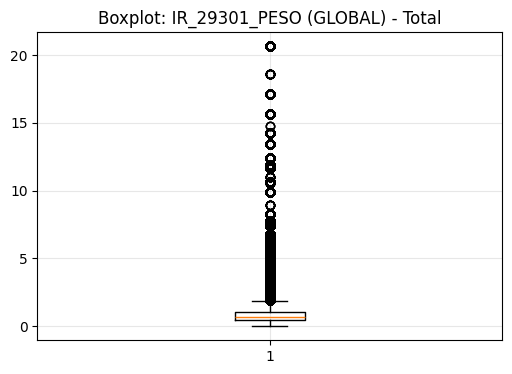
\includegraphics[width=\linewidth]{images/boxplot_global.png} % <-- Reemplaza con tu archivo
        \caption*{Población Total}
    \end{minipage}\hfill
    % Boxplot Oncológica
    \begin{minipage}{0.32\textwidth}
        \centering
        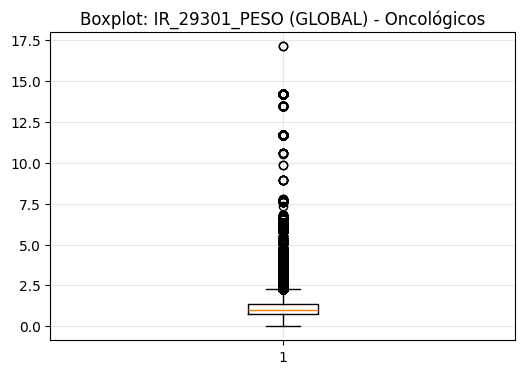
\includegraphics[width=\linewidth]{images/boxplot_oncologico.png} % <-- Reemplaza con tu archivo
        \caption*{Cohorte Oncológica}
    \end{minipage}\hfill
    % Boxplot Control
    \begin{minipage}{0.32\textwidth}
        \centering
        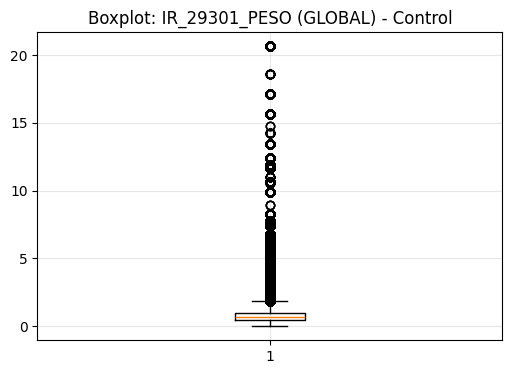
\includegraphics[width=\linewidth]{images/boxplot_control.png} % <-- Reemplaza con tu archivo
        \caption*{Grupo Control}
    \end{minipage}
    \caption{Distribución y valores atípicos del Peso Relativo GRD por cohorte de estudio.}
    \label{fig:boxplots_peso}
\end{figure}


Con el fin de validar la discretización por cuantiles (terciles) de la variable continua de peso (consumo de recursos) y así formular un problema de clasificación de tres clases ordinales, se analizó la estabilidad temporal y poblacional de los terciles como se ve en la Tabla \ref{tab:terciles_consumo}, ya que dado el severo sesgo a la derecha de la distribución, era imperativo demostrar que esta técnica matemática no generó estratos desbalanceados que puedan perjudicar el aprendizaje de los algoritmos.

Esta tabla muestra el éxito de la discretización operativa, ya que al aplicar la técnica de cortes dinámicos sobre la cohorte total, la variable objetivo logró un balanceamiento natural casi perfecto, gravitando sistemáticamente en torno al 33,3\% por categoría. Además, resulta relevante que, al segmentar y analizar exclusivamente a la cohorte oncológica, la distribución de los terciles se mantuvo excepcionalmente equilibrada (Bajo: 33,5\%, Medio: 33,4\%, Alto: 33,0\%), lo que confirma que la definición del target es estadísticamente sólida, garantizando que los modelos cuenten con un volumen equivalente de ejemplos para aprender los factores de riesgo en cada nivel de complejidad financiera, mitigando cualquier riesgo de sub representación durante la etapa de modelado.

\begin{table}[htbp]
\centering
\scriptsize
\setlength{\tabcolsep}{4pt}
\renewcommand{\arraystretch}{1.3}
\caption{Distribución de clases del Consumo de Recursos tras la discretización global (2019-2024).}
\label{tab:terciles_consumo}
\begin{tabular}{|l|c|c|c|c|c|c|}
\hline
\parbox[t]{2.5cm}{\textbf{Cohorte}} & 
\parbox[t]{2.0cm}{\centering\textbf{Nivel Bajo\\(Tercil 1)}} & 
\parbox[t]{1.5cm}{\centering\textbf{\%}} & 
\parbox[t]{2.0cm}{\centering\textbf{Nivel Medio\\(Tercil 2)}} & 
\parbox[t]{1.5cm}{\centering\textbf{\%}} & 
\parbox[t]{2.0cm}{\centering\textbf{Nivel Alto\\(Tercil 3)}} & 
\parbox[t]{1.5cm}{\centering\textbf{\%}} \\ \hline

\parbox[t]{2.5cm}{\textbf{Cohorte Total}} & \parbox[t]{2.0cm}{\raggedleft 1.922.961} & \parbox[t]{1.5cm}{\raggedleft 33,10\%} & \parbox[t]{2.0cm}{\raggedleft 1.913.233} & \parbox[t]{1.5cm}{\raggedleft 32,94\%} & \parbox[t]{2.0cm}{\raggedleft 1.972.172} & \parbox[t]{1.5cm}{\raggedleft 33,95\%} \\ \hline
\parbox[t]{2.5cm}{\textbf{Cohorte Oncológica}} & \parbox[t]{2.0cm}{\raggedleft 167.201} & \parbox[t]{1.5cm}{\raggedleft 33,53\%} & \parbox[t]{2.0cm}{\raggedleft 166.838} & \parbox[t]{1.5cm}{\raggedleft 33,46\%} & \parbox[t]{2.0cm}{\raggedleft 164.575} & \parbox[t]{1.5cm}{\raggedleft 33,00\%} \\ \hline
\parbox[t]{2.5cm}{\textbf{Grupo Control}} & \parbox[t]{2.0cm}{\raggedleft 1.859.140} & \parbox[t]{1.5cm}{\raggedleft 35,01\%} & \parbox[t]{2.0cm}{\raggedleft 1.651.087} & \parbox[t]{1.5cm}{\raggedleft 31,09\%} & \parbox[t]{2.0cm}{\raggedleft 1.799.525} & \parbox[t]{1.5cm}{\raggedleft 33,89\%} \\ \hline
\end{tabular}
\end{table}

Además del equilibrio global, era necesario demostrar que la técnica de discretización no fuera susceptible a distorsiones temporales, particularmente frente al impacto estadístico que generó la pandemia de COVID-19 sobre las medias de consumo bruto. Para ello, se auditó la distribución de los terciles año a año, como se ve en la Tabla \ref{tab:terciles_anuales_completos}, en la cual se puede observar que, a pesar de las marcadas diferencias estructurales entre la cohorte oncológica (cuya media de consumo era naturalmente superior) y la cohorte de control, la aplicación de umbrales generó divisiones virtualmente simétricas en todos los años evaluados, las cuales oscilaron entre un 31,6\% y 34,6\%, lo que confirma la estabilidad temporal de la variable objetivo y lo ideal de su uso para el modelado predictivo. Cabe mencionar que, incluso durante las caídas de ingresos registradas en la  pandemia de 2020 y 2021, donde los volúmenes absolutos disminuyeron severamente y los pesos relativos promedio aumentaron, las proporciones porcentuales dentro de cada nivel de consumo fluctuaron en un margen de error estadísticamente despreciable de $\pm 1,7\%$ respecto al tercio ideal ($33,3\%$).

Esta constancia longitudinal asegura que el aprendizaje de los algoritmos de clasificación no estará sesgado por años atípicos y valida la viabilidad de utilizar esta variable sintética como un indicador fiable para la planificación de recursos en futuros escenarios hospitalarios. 

\begin{table}[htbp]
\centering
\scriptsize
\setlength{\tabcolsep}{2pt}
\renewcommand{\arraystretch}{1.2}
\caption{Distribución anual de los niveles de Consumo de Recursos (Terciles) por cohorte (2019-2024).}
\label{tab:terciles_anuales_completos}
\begin{tabular}{|c|l|c|c|c|c|c|c|}
\hline
\parbox[t]{1.8cm}{\textbf{Nivel de Consumo}} & 
\parbox[t]{1.5cm}{\textbf{Cohorte}} & 
\parbox[t]{2cm}{\centering\textbf{2019}} & 
\parbox[t]{2cm}{\centering\textbf{2020}} & 
\parbox[t]{2cm}{\centering\textbf{2021}} & 
\parbox[t]{2cm}{\centering\textbf{2022}} & 
\parbox[t]{2cm}{\centering\textbf{2023}} & 
\parbox[t]{2cm}{\centering\textbf{2024}} \\ \hline

% NIVEL BAJO
\parbox[t]{1.8cm}{\textbf{Bajo (Tercil 1)}} 
& \parbox[t]{1.5cm}{Pob. Total} & \parbox[t]{2cm}{\raggedleft 382.292 (33,2\%)} & \parbox[t]{2cm}{\raggedleft 266.719 (34,1\%)} & \parbox[t]{2cm}{\raggedleft 269.717 (33,0\%)} & \parbox[t]{2cm}{\raggedleft 316.599 (33,9\%)} & \parbox[t]{2cm}{\raggedleft 346.173 (33,3\%)} & \parbox[t]{2cm}{\raggedleft 359.714 (33,1\%)} \\ 
\parbox[t]{1.8cm}{} 
& \parbox[t]{1.5cm}{Oncológica} & \parbox[t]{2cm}{\raggedleft 32.334 (33,1\%)} & \parbox[t]{2cm}{\raggedleft 21.927 (33,8\%)} & \parbox[t]{2cm}{\raggedleft 22.918 (33,7\%)} & \parbox[t]{2cm}{\raggedleft 26.985 (34,6\%)} & \parbox[t]{2cm}{\raggedleft 30.341 (33,5\%)} & \parbox[t]{2cm}{\raggedleft 32.722 (33,0\%)} \\ 
\parbox[t]{1.8cm}{} 
& \parbox[t]{1.5cm}{Control} & \parbox[t]{2cm}{\raggedleft 348.407 (33,1\%)} & \parbox[t]{2cm}{\raggedleft 248.329 (34,6\%)} & \parbox[t]{2cm}{\raggedleft 254.526 (34,0\%)} & \parbox[t]{2cm}{\raggedleft 294.529 (34,5\%)} & \parbox[t]{2cm}{\raggedleft 321.771 (33,9\%)} & \parbox[t]{2cm}{\raggedleft 325.952 (33,0\%)} \\ \hline

% NIVEL MEDIO
\parbox[t]{1.8cm}{\textbf{Medio (Tercil 2)}} 
& \parbox[t]{1.5cm}{Pob. Total} & \parbox[t]{2cm}{\raggedleft 378.943 (32,9\%)} & \parbox[t]{2cm}{\raggedleft 249.359 (31,9\%)} & \parbox[t]{2cm}{\raggedleft 270.321 (33,1\%)} & \parbox[t]{2cm}{\raggedleft 299.085 (32,1\%)} & \parbox[t]{2cm}{\raggedleft 340.627 (32,8\%)} & \parbox[t]{2cm}{\raggedleft 358.018 (33,0\%)} \\ 
\parbox[t]{1.8cm}{} 
& \parbox[t]{1.5cm}{Oncológica} & \parbox[t]{2cm}{\raggedleft 32.409 (33,1\%)} & \parbox[t]{2cm}{\raggedleft 21.233 (32,7\%)} & \parbox[t]{2cm}{\raggedleft 22.320 (32,9\%)} & \parbox[t]{2cm}{\raggedleft 25.725 (33,0\%)} & \parbox[t]{2cm}{\raggedleft 31.106 (34,3\%)} & \parbox[t]{2cm}{\raggedleft 34.306 (34,6\%)} \\ 
\parbox[t]{1.8cm}{} 
& \parbox[t]{1.5cm}{Control} & \parbox[t]{2cm}{\raggedleft 353.599 (33,6\%)} & \parbox[t]{2cm}{\raggedleft 226.370 (31,6\%)} & \parbox[t]{2cm}{\raggedleft 239.995 (32,0\%)} & \parbox[t]{2cm}{\raggedleft 274.435 (32,1\%)} & \parbox[t]{2cm}{\raggedleft 310.908 (32,8\%)} & \parbox[t]{2cm}{\raggedleft 327.515 (33,2\%)} \\ \hline

% NIVEL ALTO
\parbox[t]{1.8cm}{\textbf{Alto (Tercil 3)}} 
& \parbox[t]{1.5cm}{Pob. Total} & \parbox[t]{2cm}{\raggedleft 390.142 (33,9\%)} & \parbox[t]{2cm}{\raggedleft 265.833 (34,0\%)} & \parbox[t]{2cm}{\raggedleft 276.871 (33,9\%)} & \parbox[t]{2cm}{\raggedleft 317.130 (34,0\%)} & \parbox[t]{2cm}{\raggedleft 352.757 (33,9\%)} & \parbox[t]{2cm}{\raggedleft 368.066 (33,9\%)} \\ 
\parbox[t]{1.8cm}{} 
& \parbox[t]{1.5cm}{Oncológica} & \parbox[t]{2cm}{\raggedleft 33.086 (33,8\%)} & \parbox[t]{2cm}{\raggedleft 21.766 (33,5\%)} & \parbox[t]{2cm}{\raggedleft 22.688 (33,4\%)} & \parbox[t]{2cm}{\raggedleft 25.357 (32,5\%)} & \parbox[t]{2cm}{\raggedleft 29.268 (32,3\%)} & \parbox[t]{2cm}{\raggedleft 32.123 (32,4\%)} \\ 
\parbox[t]{1.8cm}{} 
& \parbox[t]{1.5cm}{Control} & \parbox[t]{2cm}{\raggedleft 351.542 (33,4\%)} & \parbox[t]{2cm}{\raggedleft 242.286 (33,8\%)} & \parbox[t]{2cm}{\raggedleft 254.462 (34,0\%)} & \parbox[t]{2cm}{\raggedleft 285.783 (33,4\%)} & \parbox[t]{2cm}{\raggedleft 316.163 (33,3\%)} & \parbox[t]{2cm}{\raggedleft 333.180 (33,8\%)} \\ \hline
\end{tabular}
\end{table}




\subsubsection{Análisis de variables numéricas de entrada}

Dentro de las variables numéricas de entrada, solo se identificaron las variables neonatales correspondientes a los pesos (en gramos) de los recién nacidos al nacer (\texttt{PESORN1} hasta \texttt{PESORN4}).
\begin{enumerate}
    \item \textbf{Pesos de recién nacidos (\texttt{PESORN1...4})}: se descartaron completamente, ya que al igual que se concluyó con las variables categóricas neonatales, la cohorte de este estudio está delimitada a episodios cuyo diagnóstico es una neoplasia maligna, y que una paciente oncológica curse un parto durante la misma hospitalización es un evento estadísticamente marginal (un outlier clínico a nivel poblacional), por ende, retener estas variables inyectaría cuatro columnas de ruido absoluto que están llenas de valores nulos y ceros (puesto que \texttt{PESORN1} hasta \texttt{PESORN4} contienen entre 99\% y 100\% de valores nulos, como se ve en la tabla \ref{tab:estadisticas_variables_neonatales}), lo cual consumiría memoria sin aportar varianza matemática que los algoritmos puedan usar para el perfilamiento.
\end{enumerate}


\begin{table}[htbp]
\centering
\scriptsize
\setlength{\tabcolsep}{3pt}
\renewcommand{\arraystretch}{1.2}
\caption{Auditoría de completitud y estadísticos descriptivos globales de variables neonatales (2019-2024).}
\label{tab:estadisticas_variables_neonatales}
\begin{tabular}{|l|c|c|c|c|c|c|}
\hline
\parbox[t]{2.6cm}{\textbf{Variable / Cohorte}} & 
\parbox[t]{1.4cm}{\centering\textbf{Total\\Episodios}} & 
\parbox[t]{2.3cm}{\centering\textbf{Valores Ausentes\\(N y \%)}} & 
\parbox[t]{0.9cm}{\centering\textbf{Ceros}} & 
\parbox[t]{1.2cm}{\centering\textbf{Media}} & 
\parbox[t]{1.2cm}{\centering\textbf{Mediana}} & 
\parbox[t]{1.2cm}{\centering\textbf{Std}} \\ \hline

\parbox[t]{2.6cm}{\texttt{PESORN1} (Pob. Total)} & \parbox[t]{1.4cm}{\raggedleft 5.808.455} & \parbox[t]{2.3cm}{\raggedleft 5.012.484 (86,30\%)} & \parbox[t]{0.9cm}{\raggedleft 60} & \parbox[t]{1.2cm}{\raggedleft 3.183,4} & \parbox[t]{1.2cm}{\raggedleft 3.268,0} & \parbox[t]{1.2cm}{\raggedleft 678,4} \\ \hline
\parbox[t]{2.6cm}{\texttt{PESORN1} (Oncológica)} & \parbox[t]{1.4cm}{\raggedleft 498.618} & \parbox[t]{2.3cm}{\raggedleft 497.982 (99,87\%)} & \parbox[t]{0.9cm}{\raggedleft 2} & \parbox[t]{1.2cm}{\raggedleft 2.978,5} & \parbox[t]{1.2cm}{\raggedleft 3.160,0} & \parbox[t]{1.2cm}{\raggedleft 819,8} \\ \hline
\parbox[t]{2.6cm}{\texttt{PESORN1} (Control)} & \parbox[t]{1.4cm}{\raggedleft 5.309.837} & \parbox[t]{2.3cm}{\raggedleft 4.514.502 (85,02\%)} & \parbox[t]{0.9cm}{\raggedleft 58} & \parbox[t]{1.2cm}{\raggedleft 3.183,5} & \parbox[t]{1.2cm}{\raggedleft 3.269,0} & \parbox[t]{1.2cm}{\raggedleft 678,2} \\ \hline
\parbox[t]{2.6cm}{\texttt{PESORN2} (Pob. Total)} & \parbox[t]{1.4cm}{\raggedleft 5.808.455} & \parbox[t]{2.3cm}{\raggedleft 5.799.859 (99,85\%)} & \parbox[t]{0.9cm}{\raggedleft 6} & \parbox[t]{1.2cm}{\raggedleft 2.259,8} & \parbox[t]{1.2cm}{\raggedleft 2.349,0} & \parbox[t]{1.2cm}{\raggedleft 642,1} \\ \hline
\parbox[t]{2.6cm}{\texttt{PESORN3} (Pob. Total)} & \parbox[t]{1.4cm}{\raggedleft 5.808.455} & \parbox[t]{2.3cm}{\raggedleft 5.808.380 ($\approx$100\%)} & \parbox[t]{0.9cm}{\raggedleft 0} & \parbox[t]{1.2cm}{\raggedleft 1.546,5} & \parbox[t]{1.2cm}{\raggedleft 1.635,0} & \parbox[t]{1.2cm}{\raggedleft 621,5} \\ \hline
\parbox[t]{2.6cm}{\texttt{PESORN4} (Pob. Total)} & \parbox[t]{1.4cm}{\raggedleft 781.911} & \parbox[t]{2.3cm}{\raggedleft 781.910 ($\approx$100\%)} & \parbox[t]{0.9cm}{\raggedleft 0} & \parbox[t]{1.2cm}{\raggedleft 780,0} & \parbox[t]{1.2cm}{\raggedleft 780,0} & \parbox[t]{1.2cm}{\centering --} \\ \hline
\end{tabular}
\end{table}

\section{Resultados del procesamiento de variables objetivo}

Luego del análisis sobre las tres variables objetivo (\textit{targets}) de mortalidad, severidad y consumo de recursos, se aplicó una depuración estricta sobre estas, aplicándose una política de exclusión completa para los registros que presentaran valores nulos o desconocidos en el desenlace hospitalario, para así garantizar la legitimidad del \textit{Ground Truth} sobre el cual aprenderán los modelos analíticos. Cabe mencionar que, los resultados del impacto de esta depuración sobre la muestra anual se detallan en la Tabla \ref{tab:auditoria_depuracion_targets}.

\begin{table}[htbp]
\centering
\scriptsize
\setlength{\tabcolsep}{4pt}
\renewcommand{\arraystretch}{1.2}
\caption{Auditoría de pérdida de datos por depuración de variables objetivo (2019-2024).}
\label{tab:auditoria_depuracion_targets}
\begin{tabular}{|c|c|c|c|}
\hline
\parbox[t]{1.5cm}{\centering\textbf{Año}} & 
\parbox[t]{3.0cm}{\centering\textbf{Episodios Iniciales}} & 
\parbox[t]{3.5cm}{\centering\textbf{Registros Eliminados\\(Target Nulo / \%)}} & 
\parbox[t]{3.0cm}{\centering\textbf{Episodios Finales\\Útiles (\textit{Dataset} Real)}} \\ \hline

\parbox[t]{1.5cm}{\centering 2019} & \parbox[t]{3.0cm}{\raggedleft 1.151.398} & \parbox[t]{3.5cm}{\raggedleft 80 (0,01\%)} & \parbox[t]{3.0cm}{\raggedleft 1.151.318} \\ \hline
\parbox[t]{1.5cm}{\centering 2020} & \parbox[t]{3.0cm}{\raggedleft 781.911} & \parbox[t]{3.5cm}{\raggedleft 23 (0,00\%)} & \parbox[t]{3.0cm}{\raggedleft 781.888} \\ \hline
\parbox[t]{1.5cm}{\centering 2021} & \parbox[t]{3.0cm}{\raggedleft 816.909} & \parbox[t]{3.5cm}{\raggedleft 0 (0,00\%)} & \parbox[t]{3.0cm}{\raggedleft 816.909} \\ \hline
\parbox[t]{1.5cm}{\centering 2022} & \parbox[t]{3.0cm}{\raggedleft 932.837} & \parbox[t]{3.5cm}{\raggedleft 23 (0,00\%)} & \parbox[t]{3.0cm}{\raggedleft 932.814} \\ \hline
\parbox[t]{1.5cm}{\centering 2023} & \parbox[t]{3.0cm}{\raggedleft 1.039.587} & \parbox[t]{3.5cm}{\raggedleft 30 (0,00\%)} & \parbox[t]{3.0cm}{\raggedleft 1.039.557} \\ \hline
\parbox[t]{1.5cm}{\centering 2024} & \parbox[t]{3.0cm}{\raggedleft 1.085.813} & \parbox[t]{3.5cm}{\raggedleft 15 (0,00\%)} & \parbox[t]{3.0cm}{\raggedleft 1.085.798} \\ \hline

\parbox[t]{1.5cm}{\centering Total} & \parbox[t]{3.0cm}{\raggedleft 5.808.455} & \parbox[t]{3.5cm}{\raggedleft 171 (0,00\%)} & \parbox[t]{3.0cm}{\raggedleft 5.808.284} \\ \hline
\end{tabular}
\end{table}

Como se observa en la Tabla \ref{tab:auditoria_depuracion_targets}, el impacto de la eliminación de registros incompletos fue estadísticamente marginal, alcanzando su punto máximo en el año 2019 con apenas 80 filas descartadas (0,01\% de la muestra). Para el resto de años, la pérdida de datos rondó el 0,00\%, consolidando un conjunto de datos analítico final de gran envergadura y con etiquetas completamente fiables. En total, de los 5.808.455 episodios iniciales, solo se eliminaron 171 registros por tener valores nulos en las variables objetivo, lo que representa una tasa de pérdida de datos del 0,00\%.

A continuación, las Tablas \ref{tab:frecuencia_mortalidad_final}, \ref{tab:frecuencia_severidad_final} y \ref{tab:frecuencia_consumo_final} presentan la distribución definitiva de las variables objetivo de Mortalidad, Severidad y Consumo de Recursos respectivamente, tras la depuración de registros con desenlaces nulos y la aplicación de cortes estocásticos (\textit{Terciles}) para la discretización del consumo.

\begin{table}[htbp]
\centering
\scriptsize
\setlength{\tabcolsep}{3pt}
\renewcommand{\arraystretch}{1.2}
\caption{Frecuencias definitivas del target Mortalidad por cohorte (2019-2024).}
\label{tab:frecuencia_mortalidad_final}
\begin{tabular}{|l|c|c|c|c|c|c|}
\hline
\parbox[t]{3.0cm}{\textbf{Clase / Cohorte}} & 
\parbox[t]{1.6cm}{\centering\textbf{2019}} & 
\parbox[t]{1.6cm}{\centering\textbf{2020}} & 
\parbox[t]{1.6cm}{\centering\textbf{2021}} & 
\parbox[t]{1.6cm}{\centering\textbf{2022}} & 
\parbox[t]{1.6cm}{\centering\textbf{2023}} & 
\parbox[t]{1.6cm}{\centering\textbf{2024}} \\ \hline

\parbox[t]{3.0cm}{\textbf{Vivo (0) - Oncológica}} & \parbox[t]{1.6cm}{\raggedleft 92.503} & \parbox[t]{1.6cm}{\raggedleft 60.463} & \parbox[t]{1.6cm}{\raggedleft 63.503} & \parbox[t]{1.6cm}{\raggedleft 73.218} & \parbox[t]{1.6cm}{\raggedleft 85.401} & \parbox[t]{1.6cm}{\raggedleft 93.144} \\ \hline
\parbox[t]{3.0cm}{\textbf{Vivo (0) - Control}} & \parbox[t]{1.6cm}{\raggedleft 1.029.231} & \parbox[t]{1.6cm}{\raggedleft 691.483} & \parbox[t]{1.6cm}{\raggedleft 721.441} & \parbox[t]{1.6cm}{\raggedleft 832.235} & \parbox[t]{1.6cm}{\raggedleft 929.034} & \parbox[t]{1.6cm}{\raggedleft 965.980} \\ \hline
\rowcolor{gray!15}\parbox[t]{3.0cm}{\textbf{Vivo (0) - Pob. Total}} & \parbox[t]{1.6cm}{\raggedleft 1.121.734} & \parbox[t]{1.6cm}{\raggedleft 751.946} & \parbox[t]{1.6cm}{\raggedleft 784.944} & \parbox[t]{1.6cm}{\raggedleft 905.453} & \parbox[t]{1.6cm}{\raggedleft 1.014.435} & \parbox[t]{1.6cm}{\raggedleft 1.059.124} \\ \hline
\parbox[t]{3.0cm}{\textbf{Fallecido (1) - Oncológica}} & \parbox[t]{1.6cm}{\raggedleft 5.321} & \parbox[t]{1.6cm}{\raggedleft 4.462} & \parbox[t]{1.6cm}{\raggedleft 4.423} & \parbox[t]{1.6cm}{\raggedleft 4.849} & \parbox[t]{1.6cm}{\raggedleft 5.314} & \parbox[t]{1.6cm}{\raggedleft 6.007} \\ \hline
\parbox[t]{3.0cm}{\textbf{Fallecido (1) - Control}} & \parbox[t]{1.6cm}{\raggedleft 24.263} & \parbox[t]{1.6cm}{\raggedleft 25.480} & \parbox[t]{1.6cm}{\raggedleft 27.542} & \parbox[t]{1.6cm}{\raggedleft 22.512} & \parbox[t]{1.6cm}{\raggedleft 19.808} & \parbox[t]{1.6cm}{\raggedleft 20.667} \\ \hline
\rowcolor{gray!15}\parbox[t]{3.0cm}{\textbf{Fallecido (1) - Pob. Total}} & \parbox[t]{1.6cm}{\raggedleft 29.584} & \parbox[t]{1.6cm}{\raggedleft 29.942} & \parbox[t]{1.6cm}{\raggedleft 31.965} & \parbox[t]{1.6cm}{\raggedleft 27.361} & \parbox[t]{1.6cm}{\raggedleft 25.122} & \parbox[t]{1.6cm}{\raggedleft 26.674} \\ \hline
\end{tabular}
\end{table}

\begin{table}[htbp]
\centering
\scriptsize
\setlength{\tabcolsep}{3pt}
\renewcommand{\arraystretch}{1.2}
\caption{Frecuencias definitivas del target Severidad (Niveles 0 al 3) por cohorte (2019-2024).}
\label{tab:frecuencia_severidad_final}
\begin{tabular}{|l|c|c|c|c|c|c|}
\hline
\parbox[t]{3.0cm}{\textbf{Nivel / Cohorte}} & 
\parbox[t]{1.6cm}{\centering\textbf{2019}} & 
\parbox[t]{1.6cm}{\centering\textbf{2020}} & 
\parbox[t]{1.6cm}{\centering\textbf{2021}} & 
\parbox[t]{1.6cm}{\centering\textbf{2022}} & 
\parbox[t]{1.6cm}{\centering\textbf{2023}} & 
\parbox[t]{1.6cm}{\centering\textbf{2024}} \\ \hline

\parbox[t]{3.0cm}{\textbf{Nivel 0 - Oncológica}} & \parbox[t]{1.6cm}{\raggedleft 20.675} & \parbox[t]{1.6cm}{\raggedleft 3.648} & \parbox[t]{1.6cm}{\raggedleft 5.689} & \parbox[t]{1.6cm}{\raggedleft 7.909} & \parbox[t]{1.6cm}{\raggedleft 10.215} & \parbox[t]{1.6cm}{\raggedleft 11.081} \\ \hline
\parbox[t]{3.0cm}{\textbf{Nivel 0 - Control}} & \parbox[t]{1.6cm}{\raggedleft 181.841} & \parbox[t]{1.6cm}{\raggedleft 76.016} & \parbox[t]{1.6cm}{\raggedleft 97.249} & \parbox[t]{1.6cm}{\raggedleft 146.863} & \parbox[t]{1.6cm}{\raggedleft 183.335} & \parbox[t]{1.6cm}{\raggedleft 200.970} \\ \hline
\rowcolor{gray!15}\parbox[t]{3.0cm}{\textbf{Nivel 0 - Pob. Total}} & \parbox[t]{1.6cm}{\raggedleft 202.516} & \parbox[t]{1.6cm}{\raggedleft 79.664} & \parbox[t]{1.6cm}{\raggedleft 102.938} & \parbox[t]{1.6cm}{\raggedleft 154.772} & \parbox[t]{1.6cm}{\raggedleft 193.550} & \parbox[t]{1.6cm}{\raggedleft 212.051} \\ \hline
\parbox[t]{3.0cm}{\textbf{Nivel 1 - Oncológica}} & \parbox[t]{1.6cm}{\raggedleft 26.703} & \parbox[t]{1.6cm}{\raggedleft 19.058} & \parbox[t]{1.6cm}{\raggedleft 19.126} & \parbox[t]{1.6cm}{\raggedleft 20.488} & \parbox[t]{1.6cm}{\raggedleft 21.770} & \parbox[t]{1.6cm}{\raggedleft 23.198} \\ \hline
\parbox[t]{3.0cm}{\textbf{Nivel 1 - Control}} & \parbox[t]{1.6cm}{\raggedleft 531.838} & \parbox[t]{1.6cm}{\raggedleft 347.220} & \parbox[t]{1.6cm}{\raggedleft 321.010} & \parbox[t]{1.6cm}{\raggedleft 352.952} & \parbox[t]{1.6cm}{\raggedleft 366.924} & \parbox[t]{1.6cm}{\raggedleft 364.060} \\ \hline
\rowcolor{gray!15}\parbox[t]{3.0cm}{\textbf{Nivel 1 - Pob. Total}} & \parbox[t]{1.6cm}{\raggedleft 558.541} & \parbox[t]{1.6cm}{\raggedleft 366.278} & \parbox[t]{1.6cm}{\raggedleft 340.136} & \parbox[t]{1.6cm}{\raggedleft 373.440} & \parbox[t]{1.6cm}{\raggedleft 388.694} & \parbox[t]{1.6cm}{\raggedleft 387.258} \\ \hline
\parbox[t]{3.0cm}{\textbf{Nivel 2 - Oncológica}} & \parbox[t]{1.6cm}{\raggedleft 30.675} & \parbox[t]{1.6cm}{\raggedleft 23.807} & \parbox[t]{1.6cm}{\raggedleft 23.718} & \parbox[t]{1.6cm}{\raggedleft 26.710} & \parbox[t]{1.6cm}{\raggedleft 31.917} & \parbox[t]{1.6cm}{\raggedleft 34.607} \\ \hline
\parbox[t]{3.0cm}{\textbf{Nivel 2 - Control}} & \parbox[t]{1.6cm}{\raggedleft 211.595} & \parbox[t]{1.6cm}{\raggedleft 152.742} & \parbox[t]{1.6cm}{\raggedleft 160.104} & \parbox[t]{1.6cm}{\raggedleft 186.550} & \parbox[t]{1.6cm}{\raggedleft 221.169} & \parbox[t]{1.6cm}{\raggedleft 234.258} \\ \hline
\rowcolor{gray!15}\parbox[t]{3.0cm}{\textbf{Nivel 2 - Pob. Total}} & \parbox[t]{1.6cm}{\raggedleft 242.270} & \parbox[t]{1.6cm}{\raggedleft 176.549} & \parbox[t]{1.6cm}{\raggedleft 183.822} & \parbox[t]{1.6cm}{\raggedleft 213.260} & \parbox[t]{1.6cm}{\raggedleft 253.086} & \parbox[t]{1.6cm}{\raggedleft 268.865} \\ \hline
\parbox[t]{3.0cm}{\textbf{Nivel 3 - Oncológica}} & \parbox[t]{1.6cm}{\raggedleft 19.771} & \parbox[t]{1.6cm}{\raggedleft 18.412} & \parbox[t]{1.6cm}{\raggedleft 19.393} & \parbox[t]{1.6cm}{\raggedleft 22.960} & \parbox[t]{1.6cm}{\raggedleft 26.813} & \parbox[t]{1.6cm}{\raggedleft 30.265} \\ \hline
\parbox[t]{3.0cm}{\textbf{Nivel 3 - Control}} & \parbox[t]{1.6cm}{\raggedleft 128.220} & \parbox[t]{1.6cm}{\raggedleft 140.985} & \parbox[t]{1.6cm}{\raggedleft 170.620} & \parbox[t]{1.6cm}{\raggedleft 168.382} & \parbox[t]{1.6cm}{\raggedleft 177.414} & \parbox[t]{1.6cm}{\raggedleft 187.359} \\ \hline
\rowcolor{gray!15}\parbox[t]{3.0cm}{\textbf{Nivel 3 - Pob. Total}} & \parbox[t]{1.6cm}{\raggedleft 147.991} & \parbox[t]{1.6cm}{\raggedleft 159.397} & \parbox[t]{1.6cm}{\raggedleft 190.013} & \parbox[t]{1.6cm}{\raggedleft 191.342} & \parbox[t]{1.6cm}{\raggedleft 204.227} & \parbox[t]{1.6cm}{\raggedleft 217.624} \\ \hline
\end{tabular}
\end{table}

\begin{table}[htbp]
\centering
\scriptsize
\setlength{\tabcolsep}{3pt}
\renewcommand{\arraystretch}{1.2}
\caption{Frecuencias definitivas del target Consumo de Recursos (Terciles 0 al 2) por cohorte.}
\label{tab:frecuencia_consumo_final}
\begin{tabular}{|l|c|c|c|c|c|c|}
\hline
\parbox[t]{3.0cm}{\textbf{Tercil / Cohorte}} & 
\parbox[t]{1.6cm}{\centering\textbf{2019}} & 
\parbox[t]{1.6cm}{\centering\textbf{2020}} & 
\parbox[t]{1.6cm}{\centering\textbf{2021}} & 
\parbox[t]{1.6cm}{\centering\textbf{2022}} & 
\parbox[t]{1.6cm}{\centering\textbf{2023}} & 
\parbox[t]{1.6cm}{\centering\textbf{2024}} \\ \hline

\parbox[t]{3.0cm}{\textbf{Tercil 0 (Bajo) - Onco}} & \parbox[t]{1.6cm}{\raggedleft 10.304} & \parbox[t]{1.6cm}{\raggedleft 4.463} & \parbox[t]{1.6cm}{\raggedleft 5.948} & \parbox[t]{1.6cm}{\raggedleft 7.038} & \parbox[t]{1.6cm}{\raggedleft 8.998} & \parbox[t]{1.6cm}{\raggedleft 10.188} \\ \hline
\parbox[t]{3.0cm}{\textbf{Tercil 0 (Bajo) - Control}} & \parbox[t]{1.6cm}{\raggedleft 374.358} & \parbox[t]{1.6cm}{\raggedleft 262.242} & \parbox[t]{1.6cm}{\raggedleft 266.729} & \parbox[t]{1.6cm}{\raggedleft 309.561} & \parbox[t]{1.6cm}{\raggedleft 338.757} & \parbox[t]{1.6cm}{\raggedleft 352.112} \\ \hline
\rowcolor{gray!15}\parbox[t]{3.0cm}{\textbf{Tercil 0 (Bajo) - Pob. Total}} & \parbox[t]{1.6cm}{\raggedleft 384.662} & \parbox[t]{1.6cm}{\raggedleft 266.705} & \parbox[t]{1.6cm}{\raggedleft 272.677} & \parbox[t]{1.6cm}{\raggedleft 316.599} & \parbox[t]{1.6cm}{\raggedleft 347.755} & \parbox[t]{1.6cm}{\raggedleft 362.300} \\ \hline
\parbox[t]{3.0cm}{\textbf{Tercil 1 (Medio) - Onco}} & \parbox[t]{1.6cm}{\raggedleft 21.605} & \parbox[t]{1.6cm}{\raggedleft 22.658} & \parbox[t]{1.6cm}{\raggedleft 24.915} & \parbox[t]{1.6cm}{\raggedleft 20.558} & \parbox[t]{1.6cm}{\raggedleft 23.684} & \parbox[t]{1.6cm}{\raggedleft 31.300} \\ \hline
\parbox[t]{3.0cm}{\textbf{Tercil 1 (Medio) - Control}} & \parbox[t]{1.6cm}{\raggedleft 363.550} & \parbox[t]{1.6cm}{\raggedleft 233.995} & \parbox[t]{1.6cm}{\raggedleft 248.701} & \parbox[t]{1.6cm}{\raggedleft 285.453} & \parbox[t]{1.6cm}{\raggedleft 322.150} & \parbox[t]{1.6cm}{\raggedleft 334.153} \\ \hline
\rowcolor{gray!15}\parbox[t]{3.0cm}{\textbf{Tercil 1 (Medio) - Pob. Total}} & \parbox[t]{1.6cm}{\raggedleft 385.155} & \parbox[t]{1.6cm}{\raggedleft 256.653} & \parbox[t]{1.6cm}{\raggedleft 273.616} & \parbox[t]{1.6cm}{\raggedleft 306.011} & \parbox[t]{1.6cm}{\raggedleft 345.834} & \parbox[t]{1.6cm}{\raggedleft 365.453} \\ \hline
\parbox[t]{3.0cm}{\textbf{Tercil 2 (Alto) - Onco}} & \parbox[t]{1.6cm}{\raggedleft 65.915} & \parbox[t]{1.6cm}{\raggedleft 37.804} & \parbox[t]{1.6cm}{\raggedleft 37.063} & \parbox[t]{1.6cm}{\raggedleft 50.471} & \parbox[t]{1.6cm}{\raggedleft 58.033} & \parbox[t]{1.6cm}{\raggedleft 57.663} \\ \hline
\parbox[t]{3.0cm}{\textbf{Tercil 2 (Alto) - Control}} & \parbox[t]{1.6cm}{\raggedleft 315.586} & \parbox[t]{1.6cm}{\raggedleft 220.726} & \parbox[t]{1.6cm}{\raggedleft 233.553} & \parbox[t]{1.6cm}{\raggedleft 259.733} & \parbox[t]{1.6cm}{\raggedleft 287.935} & \parbox[t]{1.6cm}{\raggedleft 300.382} \\ \hline
\rowcolor{gray!15}\parbox[t]{3.0cm}{\textbf{Tercil 2 (Alto) - Pob. Total}} & \parbox[t]{1.6cm}{\raggedleft 381.501} & \parbox[t]{1.6cm}{\raggedleft 258.530} & \parbox[t]{1.6cm}{\raggedleft 270.616} & \parbox[t]{1.6cm}{\raggedleft 310.204} & \parbox[t]{1.6cm}{\raggedleft 345.968} & \parbox[t]{1.6cm}{\raggedleft 358.045} \\ \hline
\end{tabular}
\end{table}

Al observar la Tabla \ref{tab:frecuencia_mortalidad_final} (Mortalidad), se verifica que la población oncológica exhibe una tasa de mortalidad significativamente más alta en comparación con el grupo de control. En general, la tasa de mortalidad para la cohorte oncológica es de 6,09\% (de $498.608$, $468.232$ sobreviven y $30.376$ fallecen), mientras que para el grupo de control es de 2,64\% (de $5.309.676$, $5.169.404$ sobreviven y $140.272$ fallecen). Cabe mencionar que, esta diferencia de tasas de mortalidad se mantiene constante a lo largo de los años, confirmando la gravedad intrínseca del cáncer como condición clínica.

Por otro lado, al inspeccionar la Tabla \ref{tab:frecuencia_consumo_final} (Consumo de Recursos), al desglosar el comportamiento interno por cohorte, se observa que la población oncológica está masivamente desplazada hacia el \textbf{Tercil 2 (Alto)}. Por ejemplo, en el año 2024, de un total de $99.151$ episodios oncológicos, $57.663$ casos (el 58,16\%) se concentraron en el estrato de mayor consumo financiero, mientras que solo un 10,28\% ($10.188$ casos) calificó en el Tercil Bajo. Por el contrario, el grupo de control exhibió un comportamiento orientado hacia el Tercil Bajo (0) de forma sistemática durante todo el periodo.

Este comportamiento confirma que el cáncer impone una huella de consumo intrínsecamente severa sobre la red asistencial, validando la necesidad de entrenar modelos predictivos capaces de aislar estas reglas de asignación presupuestaria. Asimismo, los datos de severidad (Tabla \ref{tab:frecuencia_severidad_final}) respaldan esta tendencia, ya que se consolida al Nivel 2 (severidad moderada) y Nivel 3 (severidad mayor) como los entornos normativos para el paciente oncológico (alcanzando casi el 62\% de los casos, en específico, $171.434$ casos de nivel 2 y $137.614$ casos de nivel 3), mientras que el grupo de control posee más del 59,7\% de sus casos bajo el estrato de Severidad Menor (1) y sin gravedad (0) ($886.274$ casos de nivel 0 y $2.284.004$ casos de nivel 1).

%%%%%%%%%%%%% pendiente
\section{Resultados del procesamiento de variables de entrada}
\label{sec:resultados_categoricas}

Tras la depuración de las variables objetivo, se procesaron las variables categóricas de entrada con el objetivo de reducir la alta cardinalidad de los atributos mediante agrupaciones semánticas (ingeniería de características) y aplicar exclusiones sobre aquellos episodios que presentaran valores nulos o desconocidos en los campos obligatorios, con el fin de mejorar la calidad de los datos y garantizar la fiabilidad de los modelos predictivos que se entrenarán posteriormente. En consecuencia, para validar que la limpieza no distorsionó la muestra original, se auditó la pérdida iterativa de registros desde la base inicial de $5.808.284$ episodios (obtenida tras el procesamiento de las variables objetivo), consolidando el impacto general de esta reducción de cardinalidad y depuración en la Tabla \ref{tab:resumen_limpieza_categoricas}.

% para reducir su cardinalidad y eliminar registros con valores nulos o desconocidos en campos clínicos obligatorios. 
% Este proceso se llevó a cabo con el objetivo de mejorar la calidad de los datos y garantizar la fiabilidad de los modelos predictivos que se entrenarán posteriormente.

% La fase de preparación de datos estructurados exigió un tratamiento profundo sobre las variables categóricas de entrada. Este proceso tuvo un doble objetivo: en primer lugar, reducir la alta cardinalidad de atributos administrativos y topográficos mediante agrupaciones semánticas (Ingeniería de Características) y, en segundo lugar, aplicar una política de exclusión sobre aquellos episodios que presentaran valores nulos o desconocidos en campos clínicos obligatorios. 

% Para garantizar la transparencia del estudio y validar que la limpieza no distorsionó la muestra original, se auditó la pérdida iterativa de registros desde la base inicial de $5.808.284$ episodios. El impacto general de esta reducción de cardinalidad y depuración se consolida en la Tabla \ref{tab:resumen_limpieza_categoricas}.

\begin{table}[htbp]
\centering
\scriptsize
\setlength{\tabcolsep}{2pt}
\renewcommand{\arraystretch}{1.2}
\caption{Resumen de reducción de cardinalidad y depuración anual de nulos por variable categórica.}
\label{tab:resumen_limpieza_categoricas}
\begin{tabular}{|l|c|c|c|c|c|c|c|c|c|c|}
\hline
\parbox[t]{5.5cm}{\textbf{Atributo original y procesado}} & 
\parbox[t]{1.6cm}{\centering\textbf{Cardinalidad}} & 
\parbox[t]{0.7cm}{\centering\textbf{2019}} & 
\parbox[t]{0.7cm}{\centering\textbf{2020}} & 
\parbox[t]{0.7cm}{\centering\textbf{2021}} & 
\parbox[t]{0.7cm}{\centering\textbf{2022}} & 
\parbox[t]{0.7cm}{\centering\textbf{2023}} & 
\parbox[t]{0.7cm}{\centering\textbf{2024}} & 
\parbox[t]{0.9cm}{\centering\textbf{Nulos}} & 
\parbox[t]{1.5cm}{\centering\textbf{F. restantes}} \\ \hline

\parbox[t]{5.5cm}{\texttt{SEXO} $\rightarrow$ \texttt{SEXO}} & \parbox[t]{1.6cm}{\centering 2 $\rightarrow$ 2} & \parbox[t]{0.7cm}{\raggedleft 139} & \parbox[t]{0.7cm}{\raggedleft 134} & \parbox[t]{0.7cm}{\raggedleft 63} & \parbox[t]{0.7cm}{\raggedleft 52} & \parbox[t]{0.7cm}{\raggedleft 39} & \parbox[t]{0.7cm}{\raggedleft 116} & \parbox[t]{0.9cm}{\raggedleft 543} & \parbox[t]{1.3cm}{\raggedleft 5.807.741} \\ \hline
\parbox[t]{5.5cm}{\texttt{ETNIA} $\rightarrow$ \texttt{ES\_PUEBLO\_ORIGINARIO}} & \parbox[t]{1.6cm}{\centering 12 $\rightarrow$ 2} & \parbox[t]{0.7cm}{\raggedleft 4} & \parbox[t]{0.7cm}{\raggedleft 0} & \parbox[t]{0.7cm}{\raggedleft 0} & \parbox[t]{0.7cm}{\raggedleft 0} & \parbox[t]{0.7cm}{\raggedleft 0} & \parbox[t]{0.7cm}{\raggedleft 0} & \parbox[t]{0.9cm}{\raggedleft 4} & \parbox[t]{1.3cm}{\raggedleft 5.807.737} \\ \hline
\parbox[t]{5.5cm}{\texttt{PROVINCIA} $\rightarrow$ \texttt{REGION\_RESIDENCIA}} & \parbox[t]{1.6cm}{\centering 57 $\rightarrow$ 16} & \parbox[t]{0.7cm}{\raggedleft 808} & \parbox[t]{0.7cm}{\raggedleft 623} & \parbox[t]{0.7cm}{\raggedleft 40} & \parbox[t]{0.7cm}{\raggedleft 43} & \parbox[t]{0.7cm}{\raggedleft 280} & \parbox[t]{0.7cm}{\raggedleft 393} & \parbox[t]{0.9cm}{\raggedleft 2.187} & \parbox[t]{1.3cm}{\raggedleft 5.805.550} \\ \hline
\parbox[t]{5.5cm}{\texttt{NACIONALIDAD} $\rightarrow$ \texttt{ES\_EXTRANJERO}} & \parbox[t]{1.6cm}{\centering 214 $\rightarrow$ 2} & \parbox[t]{0.7cm}{\raggedleft 20.590} & \parbox[t]{0.7cm}{\raggedleft 3.024} & \parbox[t]{0.7cm}{\raggedleft 0} & \parbox[t]{0.7cm}{\raggedleft 0} & \parbox[t]{0.7cm}{\raggedleft 0} & \parbox[t]{0.7cm}{\raggedleft 0} & \parbox[t]{0.9cm}{\raggedleft 23.614} & \parbox[t]{1.3cm}{\raggedleft 5.781.936} \\ \hline
\parbox[t]{5.5cm}{\texttt{PREVISION} $\rightarrow$ \texttt{TIPO\_PREVISION}} & \parbox[t]{1.6cm}{\centering 14 $\rightarrow$ 6} & \parbox[t]{0.7cm}{\raggedleft 3.508} & \parbox[t]{0.7cm}{\raggedleft 982} & \parbox[t]{0.7cm}{\raggedleft 9} & \parbox[t]{0.7cm}{\raggedleft 59} & \parbox[t]{0.7cm}{\raggedleft 24} & \parbox[t]{0.7cm}{\raggedleft 39} & \parbox[t]{0.9cm}{\raggedleft 4.621} & \parbox[t]{1.3cm}{\raggedleft 5.777.315} \\ \hline
\parbox[t]{5.5cm}{\texttt{SERVICIO\_SALUD} $\rightarrow$ \texttt{TIPO\_SERVICIO\_SALUD}} & \parbox[t]{1.6cm}{\centering 31 $\rightarrow$ 5} & \parbox[t]{0.7cm}{\raggedleft 7} & \parbox[t]{0.7cm}{\raggedleft 250} & \parbox[t]{0.7cm}{\raggedleft 466} & \parbox[t]{0.7cm}{\raggedleft 56} & \parbox[t]{0.7cm}{\raggedleft 723} & \parbox[t]{0.7cm}{\raggedleft 567} & \parbox[t]{0.9cm}{\raggedleft 2.069} & \parbox[t]{1.3cm}{\raggedleft 5.775.246} \\ \hline
\parbox[t]{5.5cm}{\texttt{TIPO\_PROCEDENCIA} $\rightarrow$ \texttt{TIPO\_PROCEDENCIA}} & \parbox[t]{1.6cm}{\centering 19 $\rightarrow$ 7} & \parbox[t]{0.7cm}{\raggedleft 207} & \parbox[t]{0.7cm}{\raggedleft 95} & \parbox[t]{0.7cm}{\raggedleft 3.089} & \parbox[t]{0.7cm}{\raggedleft 2} & \parbox[t]{0.7cm}{\raggedleft 2} & \parbox[t]{0.7cm}{\raggedleft 5} & \parbox[t]{0.9cm}{\raggedleft 3.400} & \parbox[t]{1.3cm}{\raggedleft 5.771.846} \\ \hline
\parbox[t]{5.5cm}{\texttt{TIPO\_INGRESO} $\rightarrow$ \texttt{TIPO\_INGRESO}} & \parbox[t]{1.6cm}{\centering 5 $\rightarrow$ 3} & \parbox[t]{0.7cm}{\raggedleft 13} & \parbox[t]{0.7cm}{\raggedleft 18} & \parbox[t]{0.7cm}{\raggedleft 1} & \parbox[t]{0.7cm}{\raggedleft 33} & \parbox[t]{0.7cm}{\raggedleft 55} & \parbox[t]{0.7cm}{\raggedleft 43} & \parbox[t]{0.9cm}{\raggedleft 163} & \parbox[t]{1.3cm}{\raggedleft 5.771.683} \\ \hline
\parbox[t]{5.5cm}{\texttt{ESPECIALIDAD\_MEDICA} $\rightarrow$ \texttt{ESPECIALIDAD\_MEDICA}} & \parbox[t]{1.6cm}{\centering 103 $\rightarrow$ 18} & \parbox[t]{0.7cm}{\raggedleft 31} & \parbox[t]{0.7cm}{\raggedleft 20} & \parbox[t]{0.7cm}{\raggedleft 0} & \parbox[t]{0.7cm}{\raggedleft 0} & \parbox[t]{0.7cm}{\raggedleft 0} & \parbox[t]{0.7cm}{\raggedleft 0} & \parbox[t]{0.9cm}{\raggedleft 51} & \parbox[t]{1.3cm}{\raggedleft 5.771.632} \\ \hline
\parbox[t]{5.5cm}{\texttt{TIPO\_ACTIVIDAD} $\rightarrow$ \texttt{TIPO\_ACTIVIDAD}} & \parbox[t]{1.6cm}{\centering 5 $\rightarrow$ 2} & \parbox[t]{0.7cm}{\raggedleft 3} & \parbox[t]{0.7cm}{\raggedleft 0} & \parbox[t]{0.7cm}{\raggedleft 0} & \parbox[t]{0.7cm}{\raggedleft 0} & \parbox[t]{0.7cm}{\raggedleft 0} & \parbox[t]{0.7cm}{\raggedleft 0} & \parbox[t]{0.9cm}{\raggedleft 3} & \parbox[t]{1.3cm}{\raggedleft 5.771.629} \\ \hline
\parbox[t]{5.5cm}{\texttt{SERVICIOINGRESO} $\rightarrow$ \texttt{SERVICIOINGRESO}} & \parbox[t]{1.6cm}{\centering 92 $\rightarrow$ 7} & \parbox[t]{0.7cm}{\raggedleft 2.781} & \parbox[t]{0.7cm}{\raggedleft 185} & \parbox[t]{0.7cm}{\raggedleft 3.653} & \parbox[t]{0.7cm}{\raggedleft 5.495} & \parbox[t]{0.7cm}{\raggedleft 7.401} & \parbox[t]{0.7cm}{\raggedleft 8.131} & \parbox[t]{0.9cm}{\raggedleft 27.646} & \parbox[t]{1.3cm}{\raggedleft 5.743.983} \\ \hline
\parbox[t]{5.5cm}{\texttt{PROCEDIMIENTO1} $\rightarrow$ \texttt{TIPO\_PROCEDIMIENTO}} & \parbox[t]{1.6cm}{\centering 3.999 $\rightarrow$ 17} & \parbox[t]{0.7cm}{\raggedleft 3} & \parbox[t]{0.7cm}{\raggedleft 0} & \parbox[t]{0.7cm}{\raggedleft 3} & \parbox[t]{0.7cm}{\raggedleft 5} & \parbox[t]{0.7cm}{\raggedleft 11} & \parbox[t]{0.7cm}{\raggedleft 13} & \parbox[t]{0.9cm}{\raggedleft 35} & \parbox[t]{1.3cm}{\raggedleft 5.743.948} \\ \hline
\end{tabular}
\end{table}

Tras la aplicación de estas transformaciones (agrupaciones y exclusión de nulos), se logró reducir la cardinalidad de las variables categóricas de entrada de manera significativa, en donde destaca la variable de nacionalidad, que se redujo de 214 categorías a un indicador binario de migración (extranjero o chileno), las especialidades médicas, que se agruparon desde 103 categorías hacia 18 macro áreas funcionales, y los procedimientos, que se consolidaron desde 3.999 códigos específicos hacia 17 categorías funcionales. Por otro lado, al evaluar la cantidad de episodios eliminados para la depuración de nulos, se concluyó que la pérdida global acumulada fue de $64.336$ episodios, lo que representa aproximadamente un $1,1\%$ del volumen inicial.

Respecto al impacto de la eliminación de filas incompletas en las variables objetivo, se verificó que la mayoría de los episodios a eliminar no estuviesen fuertemente con desenlaces clínicos específicos (como alta mortalidad o severidad extrema), lo que podría distorsionar el \textit{Ground Truth} sobre el cual aprenderán los algoritmos, en especial si se eliminan registros con desenlaces minoritaríos (como desenlace de fallecimiento). 

Para descartar este fenómeno y garantizar una auditoría transparente, se desglosó el impacto de la exclusión de nulos de manera individual para cada una de las 12 variables categóricas procesadas y se registró en distintas tablas cómo se distribuyeron las filas eliminadas en cada clase de los \textit{targets} de Mortalidad, Severidad y Consumo de Recursos, separando el efecto sobre la cohorte oncológica frente a la población de control.

Como se ven en las Tablas \ref{tab:impacto_sexo}, \ref{tab:impacto_etnia}, \ref{tab:impacto_provincia}, \ref{tab:impacto_nacionalidad}, \ref{tab:impacto_prevision}, \ref{tab:impacto_servicio_salud}, \ref{tab:impacto_tipo_procedencia}, \ref{tab:impacto_tipo_ingreso}, \ref{tab:impacto_especialidad_medica}, \ref{tab:impacto_tipo_actividad}, \ref{tab:impacto_servicio_ingreso} y \ref{tab:impacto_procedimiento}, la eliminación de nulos y valores desconocidos para cada variable implicó una pérdida de registros que no superó el 0,5\% de la muestra de $5.808.284$ tras la depuración de las variables objetivo, y en la mayoría de los casos, la pérdida fue inferior al 0,1\%. En total, tras la eliminación de los valores nulos y desconocidos, se recortaron 64.336 episodios (un 1,1\% de la muestra), en donde 3.481 episodios correspondieron a la cohorte oncológica (un 0,06\% de la muestra) y 60.545 episodios a la población de control (un 1,04\% de la muestra), por lo que se concluyó que la limpieza de nulos no distorsionó la muestra original ni introdujo un sesgo de eliminación hacia desenlaces clínicos específicos, ya que la mayoría de los episodios eliminados correspondieron a desenlaces de supervivencia (clase mayoritaria).

En específico, se analizó el impacto del procesamiento de las siguientes variables:
\begin{itemize}
    \item \textbf{Sexo:} las filas con valor \texttt{DESCONOCIDO} en el campo de sexo tuvieron una frecuencia estadísticamente marginal, representando un total de 543 episodios eliminados, que corresponde a un 0,0093\% de la muestra. Como se ve en la tabla \ref{tab:impacto_sexo}, en la cohorte oncológica, la pérdida máxima fue de 31 casos, que equivale a un 0,0005\% de los casos. Por ende, se aprobó la eliminación directa de los registros nulos, ya que no se identificó un sesgo de eliminación hacia desenlaces clínicos críticos, ya que en los casos oncológicos, la mayoría de los episodios eliminados correspondieron a desenlaces de supervivencia (que es la clase mayoritaria), casos de severidad moderada (12 episodios) y consumo de recursos alto (22 casos).
    \item \textbf{Etnia:} al principio tenía como clase mayoritaria el valor de \texttt{NINGUNO}, pero a partir de 2022, esta categoría desaparece en favor del valor \texttt{OTRO}, sin embargo, la binarización aplicada a esta variable (para indicar si un paciente es o no parte de un pueblo originario) permitió neutralizar este cambio de criterio del registro GRD, sumado que las etnias específicas representaban consistentemente menos del 2\% de la muestra anual. En relación con los registros nulos, como se ve en la tabla \ref{tab:impacto_etnia}, esta variable presentó apenas 4 episodios con valor nulo pertenecientes a la muestra control, correspondiendo a un 0,0001\% de la muestra, por lo que se aprobó la eliminación directa de los 4 registros. Además, la mayoría de los episodios eliminados correspondieron a desenlaces de supervivencia (clase mayoritaria), severidad menor (nivel 1) y consumo medio y alto (tercil 2 y 3).
    \item \textbf{Provincia (región de residencia):} la agrupación en 16 regiones de esta variable representa un punto de equilibrio óptimo para evitar problemas como la maldición de la dimensionalidad. En relación con los registros nulos, como se ve en la tabla \ref{tab:impacto_provincia}, esta variable presentó 2.187 episodios con valor nulo (un 0,0377\% de la muestra), de los cuales 103 pertenecen a la cohorte oncológica y 2.084 a la población de control (un 0,0018\% y 0.0359\% respectivamente), por lo que se aprobó la eliminación directa de los registros nulos. Además, la mayoría de los episodios eliminados corresponden a desenlaces clínicos de supervivencia (clase mayoritaria), severidad menor (nivel 1) y consumo de recursos bajo (tercil 1).
    \item \textbf{Nacionalidad (es extranjero):} la binarización de esta variable permitió reducir su cardinalidad de 214 categorías a un indicador binario de migración (extranjero o chileno), lo que es relevante para evitar problemas de dimensionalidad, considerando que la categoría \textbf{Chile} abarcaba aproximadamente un 94\% de los registros y aplicar técnicas de \textit{One-Hot Encoding} sobre las 213 categorías restantes inyectaría una cantidad masiva de columnas vacías (matrices dispersas). En relación con los registros nulos, como se ve en la tabla \ref{tab:impacto_nacionalidad}, esta variable presentó 23.614 episodios con valor nulo (un 0,4066\% de la muestra), de los cuales 1.165 pertenecen a la cohorte oncológica y 22.449 a la población de control (un 0,0201\% y 0.3874\% respectivamente), por lo que se aprobó la eliminación directa de los registros nulos. Además, la mayoría de los episodios eliminados corresponden a desenlaces clínicos de supervivencia (clase mayoritaria), severidad menor (nivel 1) y consumo de recursos bajo (tercil 1).
    \item \textbf{Previsión (tipo de previsión):} la reducción de cardinalidad de esta variable desde 14 categorías hacia 6 categorías funcionales (PRIVADO, FFAA Y ORDEN, FONASA A, B, C y D) permitió reducir la dimensionalidad del espacio de características, agrupando categorías con frecuencias cercanas al 1\% de la muestra. En relación con los registros nulos, como se ve en la tabla \ref{tab:impacto_prevision}, esta variable presentó 4.621 episodios con valor nulo (un 0,0796\% de la muestra), de los cuales 353 pertenecen a la cohorte oncológica y 4.268 a la población de control (un 0,0061\% y 0.0735\% respectivamente), por lo que se aprobó la eliminación directa de los registros nulos. Además, la mayoría de los episodios eliminados corresponden a desenlaces clínicos de supervivencia, severidad menor (nivel 1) y consumo de recursos bajo (tercil 1).
    \item \textbf{Servicio de salud (tipo de servicio de salud):} la reducción de cardinalidad de esta variable desde 31 categorías hacia 5 categorías funcionales (Macrozona Norte, RM, Centro, Centro Sur y Sur Austral) permitió disminuir la dimensionalidad del espacio de características, agrupando categorías con frecuencias entre el 1\% y 3\% de la muestra. En relación con los registros nulos, como se ve en la tabla \ref{tab:impacto_servicio_salud}, esta variable presentó 2.069 episodios con valor nulo (un 0,0356\% de la muestra), de los cuales 104 pertenecen a la cohorte oncológica y 1.965 a la población de control (un 0,0018\% y 0.0338\% respectivamente), por lo que se aprobó la eliminación directa de los registros nulos. Además, la mayoría de los episodios eliminados corresponden a desenlaces clínicos de supervivencia, severidad menor (nivel 1) y consumo de recursos alto (tercil 3).
    \item \textbf{Tipo de procedencia:} la reducción de cardinalidad de esta variable desde 19 categorías hacia 7 categorías funcionales (Ambulatorio APS, especialidad, institución cerrada, traslado privado, traslado red pública, urgencia domicilio y red primaria) permitió disminuir la dimensionalidad del espacio de características, agrupando categorías con frecuencias entre el 1\% y 2\% de la muestra. En relación con los registros nulos, como se ve en la tabla \ref{tab:impacto_procedencia}, esta variable presentó 3.400 episodios con valor nulo (un 0,0585\% de la muestra), de los cuales 87 pertenecen a la cohorte oncológica y 3.313 a la población de control (un 0,0015\% y 0.057\% respectivamente), por lo que se aprobó la eliminación directa de los registros nulos. Además, la mayoría de los episodios eliminados corresponden a desenlaces clínicos de supervivencia, severidad sin gravedad (nivel 0) y consumo de recursos bajo (tercil 1).
    \item \textbf{Tipo de ingreso:} la eliminación de valores nulos y categóricos de esta variable permitió reducir su cardinalidad desde 5 categorías hacia 3 categorías funcionales (Urgencia, Electivo y Obstetrico). En relación con los registros nulos, como se ve en la tabla \ref{tab:impacto_ingreso}, esta variable presentó 163 episodios con valor nulo (un 0,0028\% de la muestra), de los cuales 17 pertenecen a la cohorte oncológica y 146 a la población de control (un 0,0003\% y 0.0025\% respectivamente), por lo que se aprobó la eliminación directa de los registros nulos. Además, la mayoría de los episodios eliminados corresponden a desenlaces clínicos de supervivencia, severidad menor (nivel 1) y consumo de recursos medio (tercil 2).
    \item \textbf{Especialidad médica:} la reducción de cardinalidad de esta variable desde 103 categorías hacia 18 categorías funcionales permitió disminuir la dimensionalidad del espacio de características, agrupando categorías con frecuencias cercanas al 1\% de la muestra. En relación con los registros nulos, como se ve en la tabla \ref{tab:impacto_especialidad}, esta variable presentó 51 episodios con valor nulo (un 0,0009\% de la muestra), de los cuales 20 pertenecen a la cohorte oncológica y 31 a la población de control (un 0,0003\% y 0.0005\% respectivamente), por lo que se aprobó la eliminación directa de los registros nulos. Además, la mayoría de los episodios eliminados corresponden a desenlaces clínicos de supervivencia, severidad sin gravedad (nivel 0) y consumo de recursos bajo (tercil 1).
    \item \textbf{Tipo de actividad:} la agrupación de categorías permitió reducir la cardinalidad de esta variable desde 5 categorías hacia 2 categorías funcionales (Hospitalización tradicional y ambulatorio CMA), lo que permitió resolver la desaparición de categorías (como hospitalización en urgencia y diurna) en los años posteriores a 2019. En relación con los registros nulos, como se ve en la tabla \ref{tab:impacto_actividad}, esta variable presentó 3 episodios con valor nulo (un 0,00001\% de la muestra) pertenecientes a la cohorte control, por lo que se aprobó la eliminación directa de los registros nulos. Además, los 3 episodios correspondieron al desenlace de supervivencia, severidad sin gravedad (nivel 0) y consumo de recursos bajo (tercil 1).
    \item \textbf{Servicio de ingreso:} la reducción de cardinalidad de esta variable desde 92 categorías hacia 7 categorías funcionales permitió disminuir la dimensionalidad del espacio de características, agrupando categorías con frecuencias entre el 2\% y 3\% de la muestra. En relación con los registros nulos, como se ve en la tabla \ref{tab:impacto_servicio_ingreso}, esta variable presentó 27.646 episodios con valor nulo (un 0,476\% de la muestra), de los cuales 1.958 pertenecen a la cohorte oncológica y 25.688 a la población de control (un 0,0337\% y 0.4423\% respectivamente), por lo que se aprobó la eliminación directa de los registros nulos. Además, la mayoría de los episodios eliminados corresponden a desenlaces clínicos de supervivencia, severidad mayor (nivel 3) y consumo de recursos alto (tercil 3).
    \item \textbf{Procedimiento 1 (tipo de procedimiento):} la reducción de cardinalidad de esta variable desde 3.999 códigos específicos hacia 17 categorías funcionales permitió disminuir la dimensionalidad del espacio de características, agrupando categorías con frecuencias menores al 1\% de la muestra. En relación con los registros nulos, como se ve en la tabla \ref{tab:impacto_procedimiento}, esta variable presentó 35 episodios con valor nulo (un 0,0006\% de la muestra), de los cuales 3 pertenecen a la cohorte oncológica y 32 a la población de control (un 0,00005\% y 0.0006\% respectivamente), por lo que se aprobó la eliminación directa de los registros nulos. Además, la mayoría de los episodios eliminados corresponden a desenlaces clínicos de supervivencia, severidad moderada (nivel 2) y consumo de recursos alto (tercil 3).
\end{itemize}



% ----------------- TABLA 1: SEXO -----------------
\begin{table}[htbp]
\centering
\scriptsize
\setlength{\tabcolsep}{4pt}
\renewcommand{\arraystretch}{1.2}
\caption{Impacto de la exclusión de nulos en \texttt{SEXO} sobre las variables objetivo.}
\label{tab:impacto_sexo}
\begin{tabular}{|l|c|c|c|}
\hline
\parbox[t]{3.5cm}{\textbf{Variable Objetivo (Clase)}} & 
\parbox[t]{2.0cm}{\centering\textbf{Oncológico}} & 
\parbox[t]{2.0cm}{\centering\textbf{Control}} & 
\parbox[t]{2.0cm}{\centering\textbf{Total}} \\ \hline
\parbox[t]{3.5cm}{Mortalidad (0: Vivo)} & \parbox[t]{2.0cm}{\raggedleft 28} & \parbox[t]{2.0cm}{\raggedleft 484} & \parbox[t]{2.0cm}{\raggedleft 512} \\ \hline
\parbox[t]{3.5cm}{Mortalidad (1: Fallecido)} & \parbox[t]{2.0cm}{\raggedleft 3} & \parbox[t]{2.0cm}{\raggedleft 28} & \parbox[t]{2.0cm}{\raggedleft 31} \\ \hline
\parbox[t]{3.5cm}{Severidad (0: Sin gravedad)} & \parbox[t]{2.0cm}{\raggedleft 6} & \parbox[t]{2.0cm}{\raggedleft 80} & \parbox[t]{2.0cm}{\raggedleft 86} \\ \hline
\parbox[t]{3.5cm}{Severidad (1: Menor)} & \parbox[t]{2.0cm}{\raggedleft 7} & \parbox[t]{2.0cm}{\raggedleft 204} & \parbox[t]{2.0cm}{\raggedleft 211} \\ \hline
\parbox[t]{3.5cm}{Severidad (2: Moderada)} & \parbox[t]{2.0cm}{\raggedleft 12} & \parbox[t]{2.0cm}{\raggedleft 119} & \parbox[t]{2.0cm}{\raggedleft 131} \\ \hline
\parbox[t]{3.5cm}{Severidad (3: Mayor)} & \parbox[t]{2.0cm}{\raggedleft 6} & \parbox[t]{2.0cm}{\raggedleft 109} & \parbox[t]{2.0cm}{\raggedleft 115} \\ \hline
\parbox[t]{3.5cm}{Consumo (0: Bajo)} & \parbox[t]{2.0cm}{\raggedleft 2} & \parbox[t]{2.0cm}{\raggedleft 169} & \parbox[t]{2.0cm}{\raggedleft 171} \\ \hline
\parbox[t]{3.5cm}{Consumo (1: Medio)} & \parbox[t]{2.0cm}{\raggedleft 7} & \parbox[t]{2.0cm}{\raggedleft 174} & \parbox[t]{2.0cm}{\raggedleft 181} \\ \hline
\parbox[t]{3.5cm}{Consumo (2: Alto)} & \parbox[t]{2.0cm}{\raggedleft 22} & \parbox[t]{2.0cm}{\raggedleft 169} & \parbox[t]{2.0cm}{\raggedleft 191} \\ \hline
\parbox[t]{3.5cm}{\textbf{Total Filas Faltantes}} & \parbox[t]{2.0cm}{\raggedleft\textbf{31 (0.0005\%)}} & \parbox[t]{2.0cm}{\raggedleft\textbf{512 (0.0088\%)}} & \parbox[t]{2.0cm}{\raggedleft\textbf{543 (0.0093\%)}} \\ \hline
\end{tabular}
\end{table}

% ----------------- TABLA 2: ETNIA -----------------
\begin{table}[htbp]
\centering
\scriptsize
\setlength{\tabcolsep}{4pt}
\renewcommand{\arraystretch}{1.2}
\caption{Impacto de la exclusión de nulos en \texttt{ETNIA} (\texttt{ES\_PUEBLO\_ORIGINARIO}).}
\label{tab:impacto_etnia}
\begin{tabular}{|l|c|c|c|}
\hline
\parbox[t]{3.5cm}{\textbf{Variable Objetivo (Clase)}} & 
\parbox[t]{2.0cm}{\centering\textbf{Oncológico}} & 
\parbox[t]{2.0cm}{\centering\textbf{Control}} & 
\parbox[t]{2.0cm}{\centering\textbf{Total}} \\ \hline
\parbox[t]{3.5cm}{Mortalidad (0: Vivo)} & \parbox[t]{2.0cm}{\raggedleft 0} & \parbox[t]{2.0cm}{\raggedleft 3} & \parbox[t]{2.0cm}{\raggedleft 3} \\ \hline
\parbox[t]{3.5cm}{Mortalidad (1: Fallecido)} & \parbox[t]{2.0cm}{\raggedleft 0} & \parbox[t]{2.0cm}{\raggedleft 1} & \parbox[t]{2.0cm}{\raggedleft 1} \\ \hline
\parbox[t]{3.5cm}{Severidad (0: Sin gravedad)} & \parbox[t]{2.0cm}{\raggedleft 0} & \parbox[t]{2.0cm}{\raggedleft 0} & \parbox[t]{2.0cm}{\raggedleft 0} \\ \hline
\parbox[t]{3.5cm}{Severidad (1: Menor)} & \parbox[t]{2.0cm}{\raggedleft 0} & \parbox[t]{2.0cm}{\raggedleft 3} & \parbox[t]{2.0cm}{\raggedleft 3} \\ \hline
\parbox[t]{3.5cm}{Severidad (2: Moderada)} & \parbox[t]{2.0cm}{\raggedleft 0} & \parbox[t]{2.0cm}{\raggedleft 1} & \parbox[t]{2.0cm}{\raggedleft 1} \\ \hline
\parbox[t]{3.5cm}{Severidad (3: Mayor)} & \parbox[t]{2.0cm}{\raggedleft 0} & \parbox[t]{2.0cm}{\raggedleft 0} & \parbox[t]{2.0cm}{\raggedleft 0} \\ \hline
\parbox[t]{3.5cm}{Consumo (0: Bajo)} & \parbox[t]{2.0cm}{\raggedleft 0} & \parbox[t]{2.0cm}{\raggedleft 0} & \parbox[t]{2.0cm}{\raggedleft 0} \\ \hline
\parbox[t]{3.5cm}{Consumo (1: Medio)} & \parbox[t]{2.0cm}{\raggedleft 0} & \parbox[t]{2.0cm}{\raggedleft 2} & \parbox[t]{2.0cm}{\raggedleft 2} \\ \hline
\parbox[t]{3.5cm}{Consumo (2: Alto)} & \parbox[t]{2.0cm}{\raggedleft 0} & \parbox[t]{2.0cm}{\raggedleft 2} & \parbox[t]{2.0cm}{\raggedleft 2} \\ \hline
\parbox[t]{3.5cm}{\textbf{Total Filas Faltantes}} & \parbox[t]{2.0cm}{\raggedleft\textbf{0 (0\%)}} & \parbox[t]{2.0cm}{\raggedleft\textbf{4 (0.0001\%)}} & \parbox[t]{2.0cm}{\raggedleft\textbf{4 (0.0001\%)}} \\ \hline
\end{tabular}
\end{table}

% ----------------- TABLA 3: PROVINCIA -----------------
\begin{table}[htbp]
\centering
\scriptsize
\setlength{\tabcolsep}{4pt}
\renewcommand{\arraystretch}{1.2}
\caption{Impacto de la exclusión de nulos en \texttt{PROVINCIA} (\texttt{REGION\_RESIDENCIA}).}
\label{tab:impacto_provincia}
\begin{tabular}{|l|c|c|c|}
\hline
\parbox[t]{3.5cm}{\textbf{Variable Objetivo (Clase)}} & 
\parbox[t]{2.0cm}{\centering\textbf{Oncológico}} & 
\parbox[t]{2.0cm}{\centering\textbf{Control}} & 
\parbox[t]{2.0cm}{\centering\textbf{Total}} \\ \hline
\parbox[t]{3.5cm}{Mortalidad (0: Vivo)} & \parbox[t]{2.0cm}{\raggedleft 97} & \parbox[t]{2.0cm}{\raggedleft 2.022} & \parbox[t]{2.0cm}{\raggedleft 2.119} \\ \hline
\parbox[t]{3.5cm}{Mortalidad (1: Fallecido)} & \parbox[t]{2.0cm}{\raggedleft 6} & \parbox[t]{2.0cm}{\raggedleft 62} & \parbox[t]{2.0cm}{\raggedleft 68} \\ \hline
\parbox[t]{3.5cm}{Severidad (0: Sin gravedad)} & \parbox[t]{2.0cm}{\raggedleft 6} & \parbox[t]{2.0cm}{\raggedleft 545} & \parbox[t]{2.0cm}{\raggedleft 551} \\ \hline
\parbox[t]{3.5cm}{Severidad (1: Menor)} & \parbox[t]{2.0cm}{\raggedleft 54} & \parbox[t]{2.0cm}{\raggedleft 950} & \parbox[t]{2.0cm}{\raggedleft 1.004} \\ \hline
\parbox[t]{3.5cm}{Severidad (2: Moderada)} & \parbox[t]{2.0cm}{\raggedleft 25} & \parbox[t]{2.0cm}{\raggedleft 259} & \parbox[t]{2.0cm}{\raggedleft 284} \\ \hline
\parbox[t]{3.5cm}{Severidad (3: Mayor)} & \parbox[t]{2.0cm}{\raggedleft 18} & \parbox[t]{2.0cm}{\raggedleft 330} & \parbox[t]{2.0cm}{\raggedleft 348} \\ \hline
\parbox[t]{3.5cm}{Consumo (0: Bajo)} & \parbox[t]{2.0cm}{\raggedleft 10} & \parbox[t]{2.0cm}{\raggedleft 952} & \parbox[t]{2.0cm}{\raggedleft 962} \\ \hline
\parbox[t]{3.5cm}{Consumo (1: Medio)} & \parbox[t]{2.0cm}{\raggedleft 29} & \parbox[t]{2.0cm}{\raggedleft 557} & \parbox[t]{2.0cm}{\raggedleft 586} \\ \hline
\parbox[t]{3.5cm}{Consumo (2: Alto)} & \parbox[t]{2.0cm}{\raggedleft 64} & \parbox[t]{2.0cm}{\raggedleft 575} & \parbox[t]{2.0cm}{\raggedleft 639} \\ \hline
\parbox[t]{3.5cm}{\textbf{Total Filas Faltantes}} & \parbox[t]{2.0cm}{\raggedleft\textbf{103 (0.0018\%)}} & \parbox[t]{2.0cm}{\raggedleft\textbf{2.084 (0.0359\%)}} & \parbox[t]{2.0cm}{\raggedleft\textbf{2.187 (0.0377\%)}} \\ \hline
\end{tabular}
\end{table}

% ----------------- TABLA 4: NACIONALIDAD -----------------
\begin{table}[htbp]
\centering
\scriptsize
\setlength{\tabcolsep}{4pt}
\renewcommand{\arraystretch}{1.2}
\caption{Impacto de la exclusión de nulos en \texttt{NACIONALIDAD} (\texttt{ES\_EXTRANJERO}).}
\label{tab:impacto_nacionalidad}
\begin{tabular}{|l|c|c|c|}
\hline
\parbox[t]{3.5cm}{\textbf{Variable Objetivo (Clase)}} & 
\parbox[t]{2.0cm}{\centering\textbf{Oncológico}} & 
\parbox[t]{2.0cm}{\centering\textbf{Control}} & 
\parbox[t]{2.0cm}{\centering\textbf{Total}} \\ \hline
\parbox[t]{3.5cm}{Mortalidad (0: Vivo)} & \parbox[t]{2.0cm}{\raggedleft 1.039} & \parbox[t]{2.0cm}{\raggedleft 21.892} & \parbox[t]{2.0cm}{\raggedleft 22.931} \\ \hline
\parbox[t]{3.5cm}{Mortalidad (1: Fallecido)} & \parbox[t]{2.0cm}{\raggedleft 126} & \parbox[t]{2.0cm}{\raggedleft 557} & \parbox[t]{2.0cm}{\raggedleft 683} \\ \hline
\parbox[t]{3.5cm}{Severidad (0: Sin gravedad)} & \parbox[t]{2.0cm}{\raggedleft 111} & \parbox[t]{2.0cm}{\raggedleft 4.556} & \parbox[t]{2.0cm}{\raggedleft 4.667} \\ \hline
\parbox[t]{3.5cm}{Severidad (1: Menor)} & \parbox[t]{2.0cm}{\raggedleft 299} & \parbox[t]{2.0cm}{\raggedleft 11.303} & \parbox[t]{2.0cm}{\raggedleft 11.602} \\ \hline
\parbox[t]{3.5cm}{Severidad (2: Moderada)} & \parbox[t]{2.0cm}{\raggedleft 512} & \parbox[t]{2.0cm}{\raggedleft 4.405} & \parbox[t]{2.0cm}{\raggedleft 4.917} \\ \hline
\parbox[t]{3.5cm}{Severidad (3: Mayor)} & \parbox[t]{2.0cm}{\raggedleft 243} & \parbox[t]{2.0cm}{\raggedleft 2.185} & \parbox[t]{2.0cm}{\raggedleft 2.428} \\ \hline
\parbox[t]{3.5cm}{Consumo (0: Bajo)} & \parbox[t]{2.0cm}{\raggedleft 106} & \parbox[t]{2.0cm}{\raggedleft 8.736} & \parbox[t]{2.0cm}{\raggedleft 8.842} \\ \hline
\parbox[t]{3.5cm}{Consumo (1: Medio)} & \parbox[t]{2.0cm}{\raggedleft 349} & \parbox[t]{2.0cm}{\raggedleft 8.195} & \parbox[t]{2.0cm}{\raggedleft 8.544} \\ \hline
\parbox[t]{3.5cm}{Consumo (2: Alto)} & \parbox[t]{2.0cm}{\raggedleft 710} & \parbox[t]{2.0cm}{\raggedleft 5.518} & \parbox[t]{2.0cm}{\raggedleft 6.228} \\ \hline
\parbox[t]{3.5cm}{\textbf{Total Filas Faltantes}} & \parbox[t]{2.0cm}{\raggedleft\textbf{1.165 (0.0201\%)}} & \parbox[t]{2.0cm}{\raggedleft\textbf{22.449 (0.3874\%)}} & \parbox[t]{2.0cm}{\raggedleft\textbf{23.614 (0.4066\%)}} \\ \hline
\end{tabular}
\end{table}

% ----------------- TABLA 5: PREVISION -----------------
\begin{table}[htbp]
\centering
\scriptsize
\setlength{\tabcolsep}{4pt}
\renewcommand{\arraystretch}{1.2}
\caption{Impacto de la exclusión de nulos en \texttt{PREVISION} (\texttt{TIPO\_PREVISION}).}
\label{tab:impacto_prevision}
\begin{tabular}{|l|c|c|c|}
\hline
\parbox[t]{3.5cm}{\textbf{Variable Objetivo (Clase)}} & 
\parbox[t]{2.0cm}{\centering\textbf{Oncológico}} & 
\parbox[t]{2.0cm}{\centering\textbf{Control}} & 
\parbox[t]{2.0cm}{\centering\textbf{Total}} \\ \hline
\parbox[t]{3.5cm}{Mortalidad (0: Vivo)} & \parbox[t]{2.0cm}{\raggedleft 326} & \parbox[t]{2.0cm}{\raggedleft 4.081} & \parbox[t]{2.0cm}{\raggedleft 4.407} \\ \hline
\parbox[t]{3.5cm}{Mortalidad (1: Fallecido)} & \parbox[t]{2.0cm}{\raggedleft 27} & \parbox[t]{2.0cm}{\raggedleft 187} & \parbox[t]{2.0cm}{\raggedleft 214} \\ \hline
\parbox[t]{3.5cm}{Severidad (0: Sin gravedad)} & \parbox[t]{2.0cm}{\raggedleft 185} & \parbox[t]{2.0cm}{\raggedleft 424} & \parbox[t]{2.0cm}{\raggedleft 609} \\ \hline
\parbox[t]{3.5cm}{Severidad (1: Menor)} & \parbox[t]{2.0cm}{\raggedleft 59} & \parbox[t]{2.0cm}{\raggedleft 2.503} & \parbox[t]{2.0cm}{\raggedleft 2.562} \\ \hline
\parbox[t]{3.5cm}{Severidad (2: Moderada)} & \parbox[t]{2.0cm}{\raggedleft 61} & \parbox[t]{2.0cm}{\raggedleft 695} & \parbox[t]{2.0cm}{\raggedleft 756} \\ \hline
\parbox[t]{3.5cm}{Severidad (3: Mayor)} & \parbox[t]{2.0cm}{\raggedleft 48} & \parbox[t]{2.0cm}{\raggedleft 646} & \parbox[t]{2.0cm}{\raggedleft 694} \\ \hline
\parbox[t]{3.5cm}{Consumo (0: Bajo)} & \parbox[t]{2.0cm}{\raggedleft 39} & \parbox[t]{2.0cm}{\raggedleft 1.740} & \parbox[t]{2.0cm}{\raggedleft 1.779} \\ \hline
\parbox[t]{3.5cm}{Consumo (1: Medio)} & \parbox[t]{2.0cm}{\raggedleft 64} & \parbox[t]{2.0cm}{\raggedleft 1.246} & \parbox[t]{2.0cm}{\raggedleft 1.310} \\ \hline
\parbox[t]{3.5cm}{Consumo (2: Alto)} & \parbox[t]{2.0cm}{\raggedleft 250} & \parbox[t]{2.0cm}{\raggedleft 1.282} & \parbox[t]{2.0cm}{\raggedleft 1.532} \\ \hline
\parbox[t]{3.5cm}{\textbf{Total Filas Faltantes}} & \parbox[t]{2.0cm}{\raggedleft\textbf{353 (0.0061\%)}} & \parbox[t]{2.0cm}{\raggedleft\textbf{4.268 (0.0735\%)}} & \parbox[t]{2.0cm}{\raggedleft\textbf{4.621 (0.0796\%)}} \\ \hline
\end{tabular}
\end{table}

% ----------------- TABLA 6: SERVICIO_SALUD -----------------
\begin{table}[htbp]
\centering
\scriptsize
\setlength{\tabcolsep}{4pt}
\renewcommand{\arraystretch}{1.2}
\caption{Impacto de la exclusión de nulos en \texttt{SERVICIO\_SALUD} (\texttt{TIPO\_SERVICIO\_SALUD}).}
\label{tab:impacto_servicio_salud}
\begin{tabular}{|l|c|c|c|}
\hline
\parbox[t]{3.5cm}{\textbf{Variable Objetivo (Clase)}} & 
\parbox[t]{2.0cm}{\centering\textbf{Oncológico}} & 
\parbox[t]{2.0cm}{\centering\textbf{Control}} & 
\parbox[t]{2.0cm}{\centering\textbf{Total}} \\ \hline
\parbox[t]{3.5cm}{Mortalidad (0: Vivo)} & \parbox[t]{2.0cm}{\raggedleft 96} & \parbox[t]{2.0cm}{\raggedleft 1.911} & \parbox[t]{2.0cm}{\raggedleft 2.007} \\ \hline
\parbox[t]{3.5cm}{Mortalidad (1: Fallecido)} & \parbox[t]{2.0cm}{\raggedleft 8} & \parbox[t]{2.0cm}{\raggedleft 54} & \parbox[t]{2.0cm}{\raggedleft 62} \\ \hline
\parbox[t]{3.5cm}{Severidad (0: Sin gravedad)} & \parbox[t]{2.0cm}{\raggedleft 3} & \parbox[t]{2.0cm}{\raggedleft 38} & \parbox[t]{2.0cm}{\raggedleft 41} \\ \hline
\parbox[t]{3.5cm}{Severidad (1: Menor)} & \parbox[t]{2.0cm}{\raggedleft 40} & \parbox[t]{2.0cm}{\raggedleft 1.190} & \parbox[t]{2.0cm}{\raggedleft 1.230} \\ \hline
\parbox[t]{3.5cm}{Severidad (2: Moderada)} & \parbox[t]{2.0cm}{\raggedleft 32} & \parbox[t]{2.0cm}{\raggedleft 377} & \parbox[t]{2.0cm}{\raggedleft 409} \\ \hline
\parbox[t]{3.5cm}{Severidad (3: Mayor)} & \parbox[t]{2.0cm}{\raggedleft 29} & \parbox[t]{2.0cm}{\raggedleft 360} & \parbox[t]{2.0cm}{\raggedleft 389} \\ \hline
\parbox[t]{3.5cm}{Consumo (0: Bajo)} & \parbox[t]{2.0cm}{\raggedleft 5} & \parbox[t]{2.0cm}{\raggedleft 679} & \parbox[t]{2.0cm}{\raggedleft 684} \\ \hline
\parbox[t]{3.5cm}{Consumo (1: Medio)} & \parbox[t]{2.0cm}{\raggedleft 36} & \parbox[t]{2.0cm}{\raggedleft 609} & \parbox[t]{2.0cm}{\raggedleft 645} \\ \hline
\parbox[t]{3.5cm}{Consumo (2: Alto)} & \parbox[t]{2.0cm}{\raggedleft 63} & \parbox[t]{2.0cm}{\raggedleft 677} & \parbox[t]{2.0cm}{\raggedleft 740} \\ \hline
\parbox[t]{3.5cm}{\textbf{Total Filas Faltantes}} & \parbox[t]{2.0cm}{\raggedleft\textbf{104 (0.0018\%)}} & \parbox[t]{2.0cm}{\raggedleft\textbf{1.965 (0.0338\%)}} & \parbox[t]{2.0cm}{\raggedleft\textbf{2.069 (0.0356\%)}} \\ \hline
\end{tabular}
\end{table}

% ----------------- TABLA 7: TIPO_PROCEDENCIA -----------------
\begin{table}[htbp]
\centering
\scriptsize
\setlength{\tabcolsep}{4pt}
\renewcommand{\arraystretch}{1.2}
\caption{Impacto de la exclusión de nulos en \texttt{TIPO\_PROCEDENCIA}.}
\label{tab:impacto_procedencia}
\begin{tabular}{|l|c|c|c|}
\hline
\parbox[t]{3.5cm}{\textbf{Variable Objetivo (Clase)}} & 
\parbox[t]{2.0cm}{\centering\textbf{Oncológico}} & 
\parbox[t]{2.0cm}{\centering\textbf{Control}} & 
\parbox[t]{2.0cm}{\centering\textbf{Total}} \\ \hline
\parbox[t]{3.5cm}{Mortalidad (0: Vivo)} & \parbox[t]{2.0cm}{\raggedleft 87} & \parbox[t]{2.0cm}{\raggedleft 3.298} & \parbox[t]{2.0cm}{\raggedleft 3.385} \\ \hline
\parbox[t]{3.5cm}{Mortalidad (1: Fallecido)} & \parbox[t]{2.0cm}{\raggedleft 0} & \parbox[t]{2.0cm}{\raggedleft 15} & \parbox[t]{2.0cm}{\raggedleft 15} \\ \hline
\parbox[t]{3.5cm}{Severidad (0: Sin gravedad)} & \parbox[t]{2.0cm}{\raggedleft 14} & \parbox[t]{2.0cm}{\raggedleft 2.101} & \parbox[t]{2.0cm}{\raggedleft 2.115} \\ \hline
\parbox[t]{3.5cm}{Severidad (1: Menor)} & \parbox[t]{2.0cm}{\raggedleft 26} & \parbox[t]{2.0cm}{\raggedleft 851} & \parbox[t]{2.0cm}{\raggedleft 877} \\ \hline
\parbox[t]{3.5cm}{Severidad (2: Moderada)} & \parbox[t]{2.0cm}{\raggedleft 18} & \parbox[t]{2.0cm}{\raggedleft 309} & \parbox[t]{2.0cm}{\raggedleft 327} \\ \hline
\parbox[t]{3.5cm}{Severidad (3: Mayor)} & \parbox[t]{2.0cm}{\raggedleft 29} & \parbox[t]{2.0cm}{\raggedleft 52} & \parbox[t]{2.0cm}{\raggedleft 81} \\ \hline
\parbox[t]{3.5cm}{Consumo (0: Bajo)} & \parbox[t]{2.0cm}{\raggedleft 12} & \parbox[t]{2.0cm}{\raggedleft 1.466} & \parbox[t]{2.0cm}{\raggedleft 1.478} \\ \hline
\parbox[t]{3.5cm}{Consumo (1: Medio)} & \parbox[t]{2.0cm}{\raggedleft 32} & \parbox[t]{2.0cm}{\raggedleft 1.379} & \parbox[t]{2.0cm}{\raggedleft 1.411} \\ \hline
\parbox[t]{3.5cm}{Consumo (2: Alto)} & \parbox[t]{2.0cm}{\raggedleft 43} & \parbox[t]{2.0cm}{\raggedleft 468} & \parbox[t]{2.0cm}{\raggedleft 511} \\ \hline
\parbox[t]{3.5cm}{\textbf{Total Filas Faltantes}} & \parbox[t]{2.0cm}{\raggedleft\textbf{87 (0.0015\%)}} & \parbox[t]{2.0cm}{\raggedleft\textbf{3.313 (0.057\%)}} & \parbox[t]{2.0cm}{\raggedleft\textbf{3.400 (0.0585\%)}} \\ \hline
\end{tabular}
\end{table}

% ----------------- TABLA 8: TIPO_INGRESO -----------------
\begin{table}[htbp]
\centering
\scriptsize
\setlength{\tabcolsep}{4pt}
\renewcommand{\arraystretch}{1.2}
\caption{Impacto de la exclusión de nulos en \texttt{TIPO\_INGRESO}.}
\label{tab:impacto_ingreso}
\begin{tabular}{|l|c|c|c|}
\hline
\parbox[t]{3.5cm}{\textbf{Variable Objetivo (Clase)}} & 
\parbox[t]{2.0cm}{\centering\textbf{Oncológico}} & 
\parbox[t]{2.0cm}{\centering\textbf{Control}} & 
\parbox[t]{2.0cm}{\centering\textbf{Total}} \\ \hline
\parbox[t]{3.5cm}{Mortalidad (0: Vivo)} & \parbox[t]{2.0cm}{\raggedleft 17} & \parbox[t]{2.0cm}{\raggedleft 145} & \parbox[t]{2.0cm}{\raggedleft 162} \\ \hline
\parbox[t]{3.5cm}{Mortalidad (1: Fallecido)} & \parbox[t]{2.0cm}{\raggedleft 0} & \parbox[t]{2.0cm}{\raggedleft 1} & \parbox[t]{2.0cm}{\raggedleft 1} \\ \hline
\parbox[t]{3.5cm}{Severidad (0: Sin gravedad)} & \parbox[t]{2.0cm}{\raggedleft 0} & \parbox[t]{2.0cm}{\raggedleft 4} & \parbox[t]{2.0cm}{\raggedleft 4} \\ \hline
\parbox[t]{3.5cm}{Severidad (1: Menor)} & \parbox[t]{2.0cm}{\raggedleft 3} & \parbox[t]{2.0cm}{\raggedleft 68} & \parbox[t]{2.0cm}{\raggedleft 71} \\ \hline
\parbox[t]{3.5cm}{Severidad (2: Moderada)} & \parbox[t]{2.0cm}{\raggedleft 9} & \parbox[t]{2.0cm}{\raggedleft 51} & \parbox[t]{2.0cm}{\raggedleft 60} \\ \hline
\parbox[t]{3.5cm}{Severidad (3: Mayor)} & \parbox[t]{2.0cm}{\raggedleft 5} & \parbox[t]{2.0cm}{\raggedleft 23} & \parbox[t]{2.0cm}{\raggedleft 28} \\ \hline
\parbox[t]{3.5cm}{Consumo (0: Bajo)} & \parbox[t]{2.0cm}{\raggedleft 0} & \parbox[t]{2.0cm}{\raggedleft 38} & \parbox[t]{2.0cm}{\raggedleft 38} \\ \hline
\parbox[t]{3.5cm}{Consumo (1: Medio)} & \parbox[t]{2.0cm}{\raggedleft 6} & \parbox[t]{2.0cm}{\raggedleft 63} & \parbox[t]{2.0cm}{\raggedleft 69} \\ \hline
\parbox[t]{3.5cm}{Consumo (2: Alto)} & \parbox[t]{2.0cm}{\raggedleft 11} & \parbox[t]{2.0cm}{\raggedleft 45} & \parbox[t]{2.0cm}{\raggedleft 56} \\ \hline
\parbox[t]{3.5cm}{\textbf{Total Filas Faltantes}} & \parbox[t]{2.0cm}{\raggedleft\textbf{17 (0.0003\%)}} & \parbox[t]{2.0cm}{\raggedleft\textbf{146 (0.0025\%)}} & \parbox[t]{2.0cm}{\raggedleft\textbf{163 (0.0028\%)}} \\ \hline
\end{tabular}
\end{table}

% ----------------- TABLA 9: ESPECIALIDAD_MEDICA -----------------
\begin{table}[htbp]
\centering
\scriptsize
\setlength{\tabcolsep}{4pt}
\renewcommand{\arraystretch}{1.2}
\caption{Impacto de la exclusión de nulos en \texttt{ESPECIALIDAD\_MEDICA}.}
\label{tab:impacto_especialidad}
\begin{tabular}{|l|c|c|c|}
\hline
\parbox[t]{3.5cm}{\textbf{Variable Objetivo (Clase)}} & 
\parbox[t]{2.0cm}{\centering\textbf{Oncológico}} & 
\parbox[t]{2.0cm}{\centering\textbf{Control}} & 
\parbox[t]{2.0cm}{\centering\textbf{Total}} \\ \hline
\parbox[t]{3.5cm}{Mortalidad (0: Vivo)} & \parbox[t]{2.0cm}{\raggedleft 19} & \parbox[t]{2.0cm}{\raggedleft 31} & \parbox[t]{2.0cm}{\raggedleft 50} \\ \hline
\parbox[t]{3.5cm}{Mortalidad (1: Fallecido)} & \parbox[t]{2.0cm}{\raggedleft 1} & \parbox[t]{2.0cm}{\raggedleft 0} & \parbox[t]{2.0cm}{\raggedleft 1} \\ \hline
\parbox[t]{3.5cm}{Severidad (0: Sin gravedad)} & \parbox[t]{2.0cm}{\raggedleft 0} & \parbox[t]{2.0cm}{\raggedleft 23} & \parbox[t]{2.0cm}{\raggedleft 23} \\ \hline
\parbox[t]{3.5cm}{Severidad (1: Menor)} & \parbox[t]{2.0cm}{\raggedleft 7} & \parbox[t]{2.0cm}{\raggedleft 4} & \parbox[t]{2.0cm}{\raggedleft 11} \\ \hline
\parbox[t]{3.5cm}{Severidad (2: Moderada)} & \parbox[t]{2.0cm}{\raggedleft 7} & \parbox[t]{2.0cm}{\raggedleft 2} & \parbox[t]{2.0cm}{\raggedleft 9} \\ \hline
\parbox[t]{3.5cm}{Severidad (3: Mayor)} & \parbox[t]{2.0cm}{\raggedleft 6} & \parbox[t]{2.0cm}{\raggedleft 2} & \parbox[t]{2.0cm}{\raggedleft 8} \\ \hline
\parbox[t]{3.5cm}{Consumo (0: Bajo)} & \parbox[t]{2.0cm}{\raggedleft 1} & \parbox[t]{2.0cm}{\raggedleft 24} & \parbox[t]{2.0cm}{\raggedleft 25} \\ \hline
\parbox[t]{3.5cm}{Consumo (1: Medio)} & \parbox[t]{2.0cm}{\raggedleft 2} & \parbox[t]{2.0cm}{\raggedleft 5} & \parbox[t]{2.0cm}{\raggedleft 7} \\ \hline
\parbox[t]{3.5cm}{Consumo (2: Alto)} & \parbox[t]{2.0cm}{\raggedleft 17} & \parbox[t]{2.0cm}{\raggedleft 2} & \parbox[t]{2.0cm}{\raggedleft 19} \\ \hline
\parbox[t]{3.5cm}{\textbf{Total Filas Faltantes}} & \parbox[t]{2.0cm}{\raggedleft\textbf{20 (0.0003\%)}} & \parbox[t]{2.0cm}{\raggedleft\textbf{31 (0.0005\%)}} & \parbox[t]{2.0cm}{\raggedleft\textbf{51 (0.0009\%)}} \\ \hline
\end{tabular}
\end{table}

% ----------------- TABLA 10: TIPO_ACTIVIDAD -----------------
\begin{table}[htbp]
\centering
\scriptsize
\setlength{\tabcolsep}{4pt}
\renewcommand{\arraystretch}{1.2}
\caption{Impacto de la exclusión de nulos en \texttt{TIPO\_ACTIVIDAD}.}
\label{tab:impacto_actividad}
\begin{tabular}{|l|c|c|c|}
\hline
\parbox[t]{3.5cm}{\textbf{Variable Objetivo (Clase)}} & 
\parbox[t]{2.0cm}{\centering\textbf{Oncológico}} & 
\parbox[t]{2.0cm}{\centering\textbf{Control}} & 
\parbox[t]{2.0cm}{\centering\textbf{Total}} \\ \hline
\parbox[t]{3.5cm}{Mortalidad (0: Vivo)} & \parbox[t]{2.0cm}{\raggedleft 0} & \parbox[t]{2.0cm}{\raggedleft 3} & \parbox[t]{2.0cm}{\raggedleft 3} \\ \hline
\parbox[t]{3.5cm}{Mortalidad (1: Fallecido)} & \parbox[t]{2.0cm}{\raggedleft 0} & \parbox[t]{2.0cm}{\raggedleft 0} & \parbox[t]{2.0cm}{\raggedleft 0} \\ \hline
\parbox[t]{3.5cm}{Severidad (0: Sin gravedad)} & \parbox[t]{2.0cm}{\raggedleft 0} & \parbox[t]{2.0cm}{\raggedleft 3} & \parbox[t]{2.0cm}{\raggedleft 3} \\ \hline
\parbox[t]{3.5cm}{Severidad (1: Menor)} & \parbox[t]{2.0cm}{\raggedleft 0} & \parbox[t]{2.0cm}{\raggedleft 0} & \parbox[t]{2.0cm}{\raggedleft 0} \\ \hline
\parbox[t]{3.5cm}{Severidad (2: Moderada)} & \parbox[t]{2.0cm}{\raggedleft 0} & \parbox[t]{2.0cm}{\raggedleft 0} & \parbox[t]{2.0cm}{\raggedleft 0} \\ \hline
\parbox[t]{3.5cm}{Severidad (3: Mayor)} & \parbox[t]{2.0cm}{\raggedleft 0} & \parbox[t]{2.0cm}{\raggedleft 0} & \parbox[t]{2.0cm}{\raggedleft 0} \\ \hline
\parbox[t]{3.5cm}{Consumo (0: Bajo)} & \parbox[t]{2.0cm}{\raggedleft 0} & \parbox[t]{2.0cm}{\raggedleft 3} & \parbox[t]{2.0cm}{\raggedleft 3} \\ \hline
\parbox[t]{3.5cm}{Consumo (1: Medio)} & \parbox[t]{2.0cm}{\raggedleft 0} & \parbox[t]{2.0cm}{\raggedleft 0} & \parbox[t]{2.0cm}{\raggedleft 0} \\ \hline
\parbox[t]{3.5cm}{Consumo (2: Alto)} & \parbox[t]{2.0cm}{\raggedleft 0} & \parbox[t]{2.0cm}{\raggedleft 0} & \parbox[t]{2.0cm}{\raggedleft 0} \\ \hline
\parbox[t]{3.5cm}{\textbf{Total Filas Faltantes}} & \parbox[t]{2.0cm}{\raggedleft\textbf{0 (0.0000\%)}} & \parbox[t]{2.0cm}{\raggedleft\textbf{3 (0.0001\%)}} & \parbox[t]{2.0cm}{\raggedleft\textbf{3 (0.0001\%)}} \\ \hline
\end{tabular}
\end{table}

% ----------------- TABLA 11: SERVICIOINGRESO -----------------
\begin{table}[htbp]
\centering
\scriptsize
\setlength{\tabcolsep}{4pt}
\renewcommand{\arraystretch}{1.2}
\caption{Impacto de la exclusión de nulos en \texttt{SERVICIOINGRESO}.}
\label{tab:impacto_servicio_ingreso}
\begin{tabular}{|l|c|c|c|}
\hline
\parbox[t]{3.5cm}{\textbf{Variable Objetivo (Clase)}} & 
\parbox[t]{2.0cm}{\centering\textbf{Oncológico}} & 
\parbox[t]{2.0cm}{\centering\textbf{Control}} & 
\parbox[t]{2.0cm}{\centering\textbf{Total}} \\ \hline
\parbox[t]{3.5cm}{Mortalidad (0: Vivo)} & \parbox[t]{2.0cm}{\raggedleft 1.843} & \parbox[t]{2.0cm}{\raggedleft 24.420} & \parbox[t]{2.0cm}{\raggedleft 26.263} \\ \hline
\parbox[t]{3.5cm}{Mortalidad (1: Fallecido)} & \parbox[t]{2.0cm}{\raggedleft 115} & \parbox[t]{2.0cm}{\raggedleft 1.268} & \parbox[t]{2.0cm}{\raggedleft 1.383} \\ \hline
\parbox[t]{3.5cm}{Severidad (0: Sin gravedad)} & \parbox[t]{2.0cm}{\raggedleft 43} & \parbox[t]{2.0cm}{\raggedleft 2.664} & \parbox[t]{2.0cm}{\raggedleft 2.707} \\ \hline
\parbox[t]{3.5cm}{Severidad (1: Menor)} & \parbox[t]{2.0cm}{\raggedleft 480} & \parbox[t]{2.0cm}{\raggedleft 9.119} & \parbox[t]{2.0cm}{\raggedleft 9.599} \\ \hline
\parbox[t]{3.5cm}{Severidad (2: Moderada)} & \parbox[t]{2.0cm}{\raggedleft 479} & \parbox[t]{2.0cm}{\raggedleft 4.975} & \parbox[t]{2.0cm}{\raggedleft 5.454} \\ \hline
\parbox[t]{3.5cm}{Severidad (3: Mayor)} & \parbox[t]{2.0cm}{\raggedleft 956} & \parbox[t]{2.0cm}{\raggedleft 8.930} & \parbox[t]{2.0cm}{\raggedleft 9.886} \\ \hline
\parbox[t]{3.5cm}{Consumo (0: Bajo)} & \parbox[t]{2.0cm}{\raggedleft 79} & \parbox[t]{2.0cm}{\raggedleft 8.017} & \parbox[t]{2.0cm}{\raggedleft 8.096} \\ \hline
\parbox[t]{3.5cm}{Consumo (1: Medio)} & \parbox[t]{2.0cm}{\raggedleft 337} & \parbox[t]{2.0cm}{\raggedleft 7.657} & \parbox[t]{2.0cm}{\raggedleft 7.994} \\ \hline
\parbox[t]{3.5cm}{Consumo (2: Alto)} & \parbox[t]{2.0cm}{\raggedleft 1.542} & \parbox[t]{2.0cm}{\raggedleft 10.014} & \parbox[t]{2.0cm}{\raggedleft 11.556} \\ \hline
\parbox[t]{3.5cm}{\textbf{Total Filas Faltantes}} & \parbox[t]{2.0cm}{\raggedleft\textbf{1.958 (0.0337\%)}} & \parbox[t]{2.0cm}{\raggedleft\textbf{25.688 (0.4423\%)}} & \parbox[t]{2.0cm}{\raggedleft\textbf{27.646 (0.4760\%)}} \\ \hline
\end{tabular}
\end{table}

% ----------------- TABLA 12: PROCEDIMIENTO1 -----------------
\begin{table}[htbp]
\centering
\scriptsize
\setlength{\tabcolsep}{4pt}
\renewcommand{\arraystretch}{1.2}
\caption{Impacto de la exclusión de nulos en \texttt{PROCEDIMIENTO1} (\texttt{TIPO\_PROCEDIMIENTO}).}
\label{tab:impacto_procedimiento}
\begin{tabular}{|l|c|c|c|}
\hline
\parbox[t]{3.5cm}{\textbf{Variable Objetivo (Clase)}} & 
\parbox[t]{2.0cm}{\centering\textbf{Oncológico}} & 
\parbox[t]{2.0cm}{\centering\textbf{Control}} & 
\parbox[t]{2.0cm}{\centering\textbf{Total}} \\ \hline
\parbox[t]{3.5cm}{Mortalidad (0: Vivo)} & \parbox[t]{2.0cm}{\raggedleft 3} & \parbox[t]{2.0cm}{\raggedleft 32} & \parbox[t]{2.0cm}{\raggedleft 35} \\ \hline
\parbox[t]{3.5cm}{Mortalidad (1: Fallecido)} & \parbox[t]{2.0cm}{\raggedleft 0} & \parbox[t]{2.0cm}{\raggedleft 0} & \parbox[t]{2.0cm}{\raggedleft 0} \\ \hline
\parbox[t]{3.5cm}{Severidad (0: Sin gravedad)} & \parbox[t]{2.0cm}{\raggedleft 0} & \parbox[t]{2.0cm}{\raggedleft 3} & \parbox[t]{2.0cm}{\raggedleft 3} \\ \hline
\parbox[t]{3.5cm}{Severidad (1: Menor)} & \parbox[t]{2.0cm}{\raggedleft 0} & \parbox[t]{2.0cm}{\raggedleft 9} & \parbox[t]{2.0cm}{\raggedleft 9} \\ \hline
\parbox[t]{3.5cm}{Severidad (2: Moderada)} & \parbox[t]{2.0cm}{\raggedleft 2} & \parbox[t]{2.0cm}{\raggedleft 14} & \parbox[t]{2.0cm}{\raggedleft 16} \\ \hline
\parbox[t]{3.5cm}{Severidad (3: Mayor)} & \parbox[t]{2.0cm}{\raggedleft 1} & \parbox[t]{2.0cm}{\raggedleft 6} & \parbox[t]{2.0cm}{\raggedleft 7} \\ \hline
\parbox[t]{3.5cm}{Consumo (0: Bajo)} & \parbox[t]{2.0cm}{\raggedleft 0} & \parbox[t]{2.0cm}{\raggedleft 7} & \parbox[t]{2.0cm}{\raggedleft 7} \\ \hline
\parbox[t]{3.5cm}{Consumo (1: Medio)} & \parbox[t]{2.0cm}{\raggedleft 2} & \parbox[t]{2.0cm}{\raggedleft 6} & \parbox[t]{2.0cm}{\raggedleft 8} \\ \hline
\parbox[t]{3.5cm}{Consumo (2: Alto)} & \parbox[t]{2.0cm}{\raggedleft 1} & \parbox[t]{2.0cm}{\raggedleft 19} & \parbox[t]{2.0cm}{\raggedleft 20} \\ \hline
\parbox[t]{3.5cm}{\textbf{Total Filas Faltantes}} & \parbox[t]{2.0cm}{\raggedleft\textbf{3 (0.00005\%)}} & \parbox[t]{2.0cm}{\raggedleft\textbf{32 (0.0006\%)}} & \parbox[t]{2.0cm}{\raggedleft\textbf{35 (0.0006\%)}} \\ \hline
\end{tabular}
\end{table}

% \vspace{0.5cm}

%Como se evidencia tras la revisión exhaustiva de las 12 tablas anteriores, las proporciones de los registros eliminados se alinean naturalmente con las distribuciones generales de la base de datos, mitigando de forma definitiva el riesgo de sesgo artificial. Incluso en el caso de mayor impacto, correspondiente a la variable \texttt{SERVICIOINGRESO} (Tabla \ref{tab:impacto_servicio_ingreso} con $27.646$ filas removidas globalmente), la tasa de mortalidad implícita de los pacientes oncológicos descartados se situó en un 5,8\% ($115$ decesos frente a $1.843$ supervivientes), una métrica que conserva la simetría con el $\approx 6,0\%$ de letalidad basal calculada para la cohorte operativa. 

% Esta correspondencia proporcional asegura que la integridad de las variables predictivas \textit{X} y los \textit{targets} paramétricos \textit{Y} se encuentra matemáticamente lista, balanceada y libre de perturbaciones sistemáticas para la fase de modelamiento algorítmico.

\section{Resultados de la generación de variables derivadas}
\label{sec:resultados_variables_derivadas}

Para capturar la complejidad clínica y operativa se sintetizó la información granular de las matrices de diagnósticos, procedimientos y fechas para construir 7 nuevos atributos analíticos: uno categórico y 6 numéricos continuos.

\subsection{Análisis de las variables derivadas categóricas}

El primer atributo categórico derivado fue la bandera binaria \texttt{ES\_QUIRURGICO}, la cual discrimina si el episodio clínico requirió o no el ingreso a pabellón, analizando el primer código CIE-9 de la matriz de procedimientos. Como se observa en la Tabla \ref{tab:frecuencia_quirurgico}, la red pública presenta una carga marcadamente intervencionista, con una proporción de episodios quirúrgicos que escaló desde un 59,15\% en 2019 hasta consolidarse sobre el 61\% a partir de 2022.

\begin{table}[htbp]
\centering
\scriptsize
\setlength{\tabcolsep}{4pt}
\renewcommand{\arraystretch}{1.2}
\caption{Proporción anual de episodios médicos versus quirúrgicos (2019-2024).}
\label{tab:frecuencia_quirurgico}
\begin{tabular}{|l|c|c|c|c|c|c|}
\hline
\parbox[t]{2.5cm}{\textbf{Clase Operativa}} & 
\parbox[t]{1.6cm}{\centering\textbf{2019}} & 
\parbox[t]{1.6cm}{\centering\textbf{2020}} & 
\parbox[t]{1.6cm}{\centering\textbf{2021}} & 
\parbox[t]{1.6cm}{\centering\textbf{2022}} & 
\parbox[t]{1.6cm}{\centering\textbf{2023}} & 
\parbox[t]{1.6cm}{\centering\textbf{2024}} \\ \hline

\parbox[t]{2.5cm}{\textbf{0 (Médico)}} & \parbox[t]{1.6cm}{\raggedleft 458.805 (40,85\%)} & \parbox[t]{1.6cm}{\raggedleft 322.514 (41,53\%)} & \parbox[t]{1.6cm}{\raggedleft 337.260 (41,66\%)} & \parbox[t]{1.6cm}{\raggedleft 348.798 (37,62\%)} & \parbox[t]{1.6cm}{\raggedleft 386.651 (37,50\%)} & \parbox[t]{1.6cm}{\raggedleft 412.644 (38,33\%)} \\ \hline
\parbox[t]{2.5cm}{\textbf{1 (Quirúrgico)}} & \parbox[t]{1.6cm}{\raggedleft 664.419 (59,15\%)} & \parbox[t]{1.6cm}{\raggedleft 454.043 (58,47\%)} & \parbox[t]{1.6cm}{\raggedleft 472.325 (58,34\%)} & \parbox[t]{1.6cm}{\raggedleft 578.271 (62,38\%)} & \parbox[t]{1.6cm}{\raggedleft 644.371 (62,50\%)} & \parbox[t]{1.6cm}{\raggedleft 663.847 (61,67\%)} \\ \hline
\end{tabular}
\end{table}

El segundo atributo, \texttt{COMORBILIDAD\_PRINCIPAL}, se diseñó de manera exclusiva para perfilar a la cohorte oncológica, mapeando la macro-categoría CIE-10 de su patología concomitante más relevante. Como lo demuestra la Tabla \ref{tab:frecuencia_comorbilidad}, más del 90\% del \textit{dataset} se etiqueta como \texttt{NO\_APLICA} al corresponder al grupo de control. Dentro de los pacientes oncológicos, destacan como comorbilidades dominantes las enfermedades del \textbf{Sistema Circulatorio} (creciendo de un 1,58\% a un 1,70\%), seguidas por los trastornos del \textbf{Sistema Digestivo} y las enfermedades \textbf{Endocrinas y Metabólicas}, evidenciando el alto grado de pluripatología que acompaña al cáncer.
\begin{table}[htbp]
\centering
\scriptsize
\setlength{\tabcolsep}{2pt}
\renewcommand{\arraystretch}{1.15}
\caption{Distribución anual exhaustiva de la variable derivada Comorbilidad Principal (2019-2024).}
\label{tab:frecuencia_comorbilidad_completa}
\begin{tabular}{|l|c|c|c|c|c|c|}
\hline
\parbox[t]{3.8cm}{\textbf{Macro-Categoría CIE-10}} &
\parbox[t]{1.5cm}{\centering\textbf{2019}} &
\parbox[t]{1.5cm}{\centering\textbf{2020}} &
\parbox[t]{1.5cm}{\centering\textbf{2021}} &
\parbox[t]{1.5cm}{\centering\textbf{2022}} &
\parbox[t]{1.5cm}{\centering\textbf{2023}} &
\parbox[t]{1.5cm}{\centering\textbf{2024}} \\ \hline

\parbox[t]{3.8cm}{Códigos Prov. (COVID-19)} & \parbox[t]{1.5cm}{\raggedleft 50 (0,00\%)} & \parbox[t]{1.5cm}{\raggedleft 1.420 (0,18\%)} & \parbox[t]{1.5cm}{\raggedleft 1.748 (0,22\%)} & \parbox[t]{1.5cm}{\raggedleft 1.608 (0,17\%)} & \parbox[t]{1.5cm}{\raggedleft 584 (0,06\%)} & \parbox[t]{1.5cm}{\raggedleft 371 (0,03\%)} \\ \hline
\parbox[t]{3.8cm}{Endocrinas y Metabólicas} & \parbox[t]{1.5cm}{\raggedleft 8.453 (0,75\%)} & \parbox[t]{1.5cm}{\raggedleft 5.423 (0,70\%)} & \parbox[t]{1.5cm}{\raggedleft 6.474 (0,80\%)} & \parbox[t]{1.5cm}{\raggedleft 7.559 (0,82\%)} & \parbox[t]{1.5cm}{\raggedleft 8.912 (0,86\%)} & \parbox[t]{1.5cm}{\raggedleft 9.822 (0,91\%)} \\ \hline
\parbox[t]{3.8cm}{Infecciosas y Parasitarias} & \parbox[t]{1.5cm}{\raggedleft 2.291 (0,20\%)} & \parbox[t]{1.5cm}{\raggedleft 1.779 (0,23\%)} & \parbox[t]{1.5cm}{\raggedleft 1.758 (0,22\%)} & \parbox[t]{1.5cm}{\raggedleft 1.971 (0,21\%)} & \parbox[t]{1.5cm}{\raggedleft 2.419 (0,23\%)} & \parbox[t]{1.5cm}{\raggedleft 2.674 (0,25\%)} \\ \hline
\parbox[t]{3.8cm}{Materno-Infantiles y Cong.} & \parbox[t]{1.5cm}{\raggedleft 573 (0,05\%)} & \parbox[t]{1.5cm}{\raggedleft 477 (0,06\%)} & \parbox[t]{1.5cm}{\raggedleft 377 (0,05\%)} & \parbox[t]{1.5cm}{\raggedleft 517 (0,06\%)} & \parbox[t]{1.5cm}{\raggedleft 579 (0,06\%)} & \parbox[t]{1.5cm}{\raggedleft 575 (0,05\%)} \\ \hline
\parbox[t]{3.8cm}{No Aplica (Grupo Control)} & \parbox[t]{1.5cm}{\raggedleft 1.026.821 (91,42\%)} & \parbox[t]{1.5cm}{\raggedleft 711.905 (91,67\%)} & \parbox[t]{1.5cm}{\raggedleft 741.800 (91,63\%)} & \parbox[t]{1.5cm}{\raggedleft 849.540 (91,64\%)} & \parbox[t]{1.5cm}{\raggedleft 940.943 (91,26\%)} & \parbox[t]{1.5cm}{\raggedleft 978.172 (90,87\%)} \\ \hline
\parbox[t]{3.8cm}{Ojo y Oído} & \parbox[t]{1.5cm}{\raggedleft 1.067 (0,09\%)} & \parbox[t]{1.5cm}{\raggedleft 541 (0,07\%)} & \parbox[t]{1.5cm}{\raggedleft 655 (0,08\%)} & \parbox[t]{1.5cm}{\raggedleft 1.033 (0,11\%)} & \parbox[t]{1.5cm}{\raggedleft 1.292 (0,13\%)} & \parbox[t]{1.5cm}{\raggedleft 1.323 (0,12\%)} \\ \hline
\parbox[t]{3.8cm}{Piel y Tejido Subcutáneo} & \parbox[t]{1.5cm}{\raggedleft 912 (0,08\%)} & \parbox[t]{1.5cm}{\raggedleft 647 (0,08\%)} & \parbox[t]{1.5cm}{\raggedleft 659 (0,08\%)} & \parbox[t]{1.5cm}{\raggedleft 714 (0,08\%)} & \parbox[t]{1.5cm}{\raggedleft 878 (0,09\%)} & \parbox[t]{1.5cm}{\raggedleft 1.092 (0,10\%)} \\ \hline
\parbox[t]{3.8cm}{Sangre e Inmunidad} & \parbox[t]{1.5cm}{\raggedleft 5.989 (0,53\%)} & \parbox[t]{1.5cm}{\raggedleft 4.510 (0,58\%)} & \parbox[t]{1.5cm}{\raggedleft 4.263 (0,53\%)} & \parbox[t]{1.5cm}{\raggedleft 4.706 (0,51\%)} & \parbox[t]{1.5cm}{\raggedleft 5.558 (0,54\%)} & \parbox[t]{1.5cm}{\raggedleft 6.329 (0,59\%)} \\ \hline
\parbox[t]{3.8cm}{Síntomas y Hallazgos} & \parbox[t]{1.5cm}{\raggedleft 2.942 (0,26\%)} & \parbox[t]{1.5cm}{\raggedleft 2.378 (0,31\%)} & \parbox[t]{1.5cm}{\raggedleft 2.543 (0,31\%)} & \parbox[t]{1.5cm}{\raggedleft 2.789 (0,30\%)} & \parbox[t]{1.5cm}{\raggedleft 3.261 (0,32\%)} & \parbox[t]{1.5cm}{\raggedleft 3.691 (0,34\%)} \\ \hline
\parbox[t]{3.8cm}{Sin Comorbilidad (Onco puro)} & \parbox[t]{1.5cm}{\raggedleft 25.182 (2,24\%)} & \parbox[t]{1.5cm}{\raggedleft 12.244 (1,58\%)} & \parbox[t]{1.5cm}{\raggedleft 11.788 (1,46\%)} & \parbox[t]{1.5cm}{\raggedleft 12.438 (1,34\%)} & \parbox[t]{1.5cm}{\raggedleft 13.579 (1,32\%)} & \parbox[t]{1.5cm}{\raggedleft 12.915 (1,20\%)} \\ \hline
\parbox[t]{3.8cm}{Sistema Circulatorio} & \parbox[t]{1.5cm}{\raggedleft 17.781 (1,58\%)} & \parbox[t]{1.5cm}{\raggedleft 11.798 (1,52\%)} & \parbox[t]{1.5cm}{\raggedleft 12.597 (1,56\%)} & \parbox[t]{1.5cm}{\raggedleft 14.701 (1,59\%)} & \parbox[t]{1.5cm}{\raggedleft 16.605 (1,61\%)} & \parbox[t]{1.5cm}{\raggedleft 18.280 (1,70\%)} \\ \hline
\parbox[t]{3.8cm}{Sistema Digestivo} & \parbox[t]{1.5cm}{\raggedleft 8.427 (0,75\%)} & \parbox[t]{1.5cm}{\raggedleft 7.243 (0,93\%)} & \parbox[t]{1.5cm}{\raggedleft 7.991 (0,99\%)} & \parbox[t]{1.5cm}{\raggedleft 8.947 (0,97\%)} & \parbox[t]{1.5cm}{\raggedleft 11.131 (1,08\%)} & \parbox[t]{1.5cm}{\raggedleft 12.088 (1,12\%)} \\ \hline
\parbox[t]{3.8cm}{Sistema Genitourinario} & \parbox[t]{1.5cm}{\raggedleft 5.779 (0,51\%)} & \parbox[t]{1.5cm}{\raggedleft 4.513 (0,58\%)} & \parbox[t]{1.5cm}{\raggedleft 5.286 (0,65\%)} & \parbox[t]{1.5cm}{\raggedleft 6.116 (0,66\%)} & \parbox[t]{1.5cm}{\raggedleft 7.268 (0,70\%)} & \parbox[t]{1.5cm}{\raggedleft 8.462 (0,79\%)} \\ \hline
\parbox[t]{3.8cm}{Sistema Músculoesquelético} & \parbox[t]{1.5cm}{\raggedleft 1814 (0,16\%)} & \parbox[t]{1.5cm}{\raggedleft 1.353 (0,17\%)} & \parbox[t]{1.5cm}{\raggedleft 1.436 (0,18\%)} & \parbox[t]{1.5cm}{\raggedleft 1.802 (0,19\%)} & \parbox[t]{1.5cm}{\raggedleft 2.310 (0,22\%)} & \parbox[t]{1.5cm}{\raggedleft 2.482 (0,23\%)} \\ \hline
\parbox[t]{3.8cm}{Sistema Nervioso} & \parbox[t]{1.5cm}{\raggedleft 1.863 (0,17\%)} & \parbox[t]{1.5cm}{\raggedleft 1.410 (0,18\%)} & \parbox[t]{1.5cm}{\raggedleft 1.471 (0,18\%)} & \parbox[t]{1.5cm}{\raggedleft 1.620 (0,17\%)} & \parbox[t]{1.5cm}{\raggedleft 1.961 (0,19\%)} & \parbox[t]{1.5cm}{\raggedleft 2.287 (0,21\%)} \\ \hline
\parbox[t]{3.8cm}{Sistema Respiratorio} & \parbox[t]{1.5cm}{\raggedleft 6.944 (0,62\%)} & \parbox[t]{1.5cm}{\raggedleft 4.455 (0,57\%)} & \parbox[t]{1.5cm}{\raggedleft 4.033 (0,50\%)} & \parbox[t]{1.5cm}{\raggedleft 5.486 (0,59\%)} & \parbox[t]{1.5cm}{\raggedleft 7.129 (0,69\%)} & \parbox[t]{1.5cm}{\raggedleft 8.377 (0,78\%)} \\ \hline
\parbox[t]{3.8cm}{Trastornos Mentales} & \parbox[t]{1.5cm}{\raggedleft 2.908 (0,26\%)} & \parbox[t]{1.5cm}{\raggedleft 1.570 (0,20\%)} & \parbox[t]{1.5cm}{\raggedleft 1.564 (0,19\%)} & \parbox[t]{1.5cm}{\raggedleft 1.774 (0,19\%)} & \parbox[t]{1.5cm}{\raggedleft 2.034 (0,20\%)} & \parbox[t]{1.5cm}{\raggedleft 2.269 (0,21\%)} \\ \hline
\parbox[t]{3.8cm}{Traumatismos y Enven.} & \parbox[t]{1.5cm}{\raggedleft 3.428 (0,31\%)} & \parbox[t]{1.5cm}{\raggedleft 2.891 (0,37\%)} & \parbox[t]{1.5cm}{\raggedleft 3.142 (0,39\%)} & \parbox[t]{1.5cm}{\raggedleft 3.748 (0,40\%)} & \parbox[t]{1.5cm}{\raggedleft 4.579 (0,44\%)} & \parbox[t]{1.5cm}{\raggedleft 5.282 (0,49\%)} \\ \hline
\end{tabular}
\end{table}

\subsection{Comportamiento de las Variables Numéricas Derivadas}

Para dimensionar la densidad de la hospitalización, se calcularon seis variables continuas: la edad empírica al ingreso (\texttt{EDAD}), la duración real del episodio (\texttt{DIAS\_ESTADIA}), la movilidad interna (\texttt{CANTIDAD\_TRASLADOS}), la densidad intervencionista (\texttt{NUM\_PROCEDIMIENTOS}), la morbilidad (\texttt{NUM\_COMORBILIDADES}) y la dispersión tumoral (\texttt{CARGA\_ONCOLOGICA}). La Tabla \ref{tab:estadisticas_numericas_derivadas} resume sus estadísticos de tendencia central y dispersión.

\begin{table}[htbp]
\centering
\scriptsize
\setlength{\tabcolsep}{4pt}
\renewcommand{\arraystretch}{1.2}
\caption{Estadística descriptiva de las variables numéricas derivadas (resumen 2019 vs 2024).}
\label{tab:estadisticas_numericas_derivadas}
\begin{tabular}{|l|c|c|c|c|c|c|}
\hline
\parbox[t]{3.0cm}{\textbf{Variable Derivada}} & 
\parbox[t]{1.5cm}{\centering\textbf{Año}} & 
\parbox[t]{1.5cm}{\centering\textbf{Mín - Máx}} & 
\parbox[t]{1.5cm}{\centering\textbf{Media}} & 
\parbox[t]{1.5cm}{\centering\textbf{Std}} & 
\parbox[t]{1.5cm}{\centering\textbf{Outliers (N)}} & 
\parbox[t]{1.5cm}{\centering\textbf{Outliers (\%)}} \\ \hline

\parbox[t]{3.0cm}{\multirow{2}{*}{\texttt{CANTIDAD\_TRASLADOS}}} & \parbox[t]{1.5cm}{\centering 2019} & \parbox[t]{1.5cm}{\centering 0 - 9} & \parbox[t]{1.5cm}{\raggedleft 0,22} & \parbox[t]{1.5cm}{\raggedleft 0,62} & \parbox[t]{1.5cm}{\raggedleft 164.536} & \parbox[t]{1.5cm}{\raggedleft 14,65\%} \\ 
\parbox[t]{3.0cm}{} & \parbox[t]{1.5cm}{\centering 2024} & \parbox[t]{1.5cm}{\centering 0 - 9} & \parbox[t]{1.5cm}{\raggedleft 0,24} & \parbox[t]{1.5cm}{\raggedleft 0,65} & \parbox[t]{1.5cm}{\raggedleft 170.890} & \parbox[t]{1.5cm}{\raggedleft 15,87\%} \\ \hline

\parbox[t]{3.0cm}{\multirow{2}{*}{\texttt{NUM\_PROCEDIMIENTOS}}} & \parbox[t]{1.5cm}{\centering 2019} & \parbox[t]{1.5cm}{\centering 0 - 30} & \parbox[t]{1.5cm}{\raggedleft 6,75} & \parbox[t]{1.5cm}{\raggedleft 5,26} & \parbox[t]{1.5cm}{\raggedleft 42.307} & \parbox[t]{1.5cm}{\raggedleft 3,77\%} \\ 
\parbox[t]{3.0cm}{} & \parbox[t]{1.5cm}{\centering 2024} & \parbox[t]{1.5cm}{\centering 0 - 30} & \parbox[t]{1.5cm}{\raggedleft 8,00} & \parbox[t]{1.5cm}{\raggedleft 6,12} & \parbox[t]{1.5cm}{\raggedleft 35.744} & \parbox[t]{1.5cm}{\raggedleft 3,32\%} \\ \hline

\parbox[t]{3.0cm}{\multirow{2}{*}{\texttt{NUM\_COMORBILIDADES}}} & \parbox[t]{1.5cm}{\centering 2019} & \parbox[t]{1.5cm}{\centering 0 - 35} & \parbox[t]{1.5cm}{\raggedleft 3,19} & \parbox[t]{1.5cm}{\raggedleft 2,76} & \parbox[t]{1.5cm}{\raggedleft 54.551} & \parbox[t]{1.5cm}{\raggedleft 4,86\%} \\ 
\parbox[t]{3.0cm}{} & \parbox[t]{1.5cm}{\centering 2024} & \parbox[t]{1.5cm}{\centering 0 - 35} & \parbox[t]{1.5cm}{\raggedleft 4,32} & \parbox[t]{1.5cm}{\raggedleft 3,77} & \parbox[t]{1.5cm}{\raggedleft 43.551} & \parbox[t]{1.5cm}{\raggedleft 4,05\%} \\ \hline

\parbox[t]{3.0cm}{\multirow{2}{*}{\texttt{CARGA\_ONCOLOGICA}}} & \parbox[t]{1.5cm}{\centering 2019} & \parbox[t]{1.5cm}{\centering 0 - 8} & \parbox[t]{1.5cm}{\raggedleft 0,15} & \parbox[t]{1.5cm}{\raggedleft 0,45} & \parbox[t]{1.5cm}{\raggedleft 136.375} & \parbox[t]{1.5cm}{\raggedleft 12,14\%} \\ 
\parbox[t]{3.0cm}{} & \parbox[t]{1.5cm}{\centering 2024} & \parbox[t]{1.5cm}{\centering 0 - 10} & \parbox[t]{1.5cm}{\raggedleft 0,17} & \parbox[t]{1.5cm}{\raggedleft 0,50} & \parbox[t]{1.5cm}{\raggedleft 144.511} & \parbox[t]{1.5cm}{\raggedleft 13,42\%} \\ \hline

\parbox[t]{3.0cm}{\multirow{2}{*}{\texttt{EDAD} (Años)}} & \parbox[t]{1.5cm}{\centering 2019} & \parbox[t]{1.5cm}{\centering 0 - 124} & \parbox[t]{1.5cm}{\raggedleft 43,09} & \parbox[t]{1.5cm}{\raggedleft 25,86} & \parbox[t]{1.5cm}{\raggedleft 0} & \parbox[t]{1.5cm}{\raggedleft 0,00\%} \\ 
\parbox[t]{3.0cm}{} & \parbox[t]{1.5cm}{\centering 2024} & \parbox[t]{1.5cm}{\centering 0 - 108} & \parbox[t]{1.5cm}{\raggedleft 45,68} & \parbox[t]{1.5cm}{\raggedleft 25,45} & \parbox[t]{1.5cm}{\raggedleft 0} & \parbox[t]{1.5cm}{\raggedleft 0,00\%} \\ \hline

\parbox[t]{3.0cm}{\multirow{2}{*}{\texttt{DIAS\_ESTADIA}}} & \parbox[t]{1.5cm}{\centering 2019} & \parbox[t]{1.5cm}{\centering 0 - 2322} & \parbox[t]{1.5cm}{\raggedleft 5,29} & \parbox[t]{1.5cm}{\raggedleft 12,80} & \parbox[t]{1.5cm}{\raggedleft 121.998} & \parbox[t]{1.5cm}{\raggedleft 10,86\%} \\ 
\parbox[t]{3.0cm}{} & \parbox[t]{1.5cm}{\centering 2024} & \parbox[t]{1.5cm}{\centering 0 - 645} & \parbox[t]{1.5cm}{\raggedleft 5,64} & \parbox[t]{1.5cm}{\raggedleft 12,02} & \parbox[t]{1.5cm}{\raggedleft 106.661} & \parbox[t]{1.5cm}{\raggedleft 9,91\%} \\ \hline
\end{tabular}
\end{table}

El análisis descriptivo revela un aumento sistémico en la densidad hospitalaria: la cantidad media de procedimientos escaló de $6,75$ a $8,00$ por episodio, mientras que la cantidad de comorbilidades documentadas ascendió de $3,19$ a $4,32$. Esto sugiere no solo un envejecimiento progresivo de la población admitida (cuya media etaria pasó de 43 a casi 46 años), sino también una mejora en la exhaustividad del registro clínico por parte del personal de salud a nivel nacional.

\subsection{Depuración de Anomalías Temporales}

La derivación matemática de las variables cronológicas (\texttt{EDAD} y \texttt{DIAS\_ESTADIA}) permitió someter a prueba la consistencia empírica de las fechas de ingreso, nacimiento y alta hospitalaria. El escaneo de sustracción detectó la presencia de valores lógicamente imposibles (estadías o edades con resultado negativo). Como se documenta en la Tabla \ref{tab:limpieza_fechas}, este fenómeno correspondió a errores reales de digitación en los sistemas de admisión hospitalaria (por ejemplo, registrar una fecha de alta anterior a la fecha de ingreso).

Dado que los algoritmos paramétricos son altamente sensibles a valores continuos negativos en métricas de duración, estos registros corruptos fueron forzados a valores nulos (NaN) y posteriormente eliminados del \textit{dataset} final. 

\begin{table}[htbp]
\centering
\scriptsize
\setlength{\tabcolsep}{4pt}
\renewcommand{\arraystretch}{1.2}
\caption{Auditoría de eliminación de episodios con anomalías cronológicas (Edades y Estadías negativas).}
\label{tab:limpieza_fechas}
\begin{tabular}{|c|c|c|c|c|}
\hline
\parbox[t]{1.5cm}{\centering\textbf{Año}} & 
\parbox[t]{3.0cm}{\centering\textbf{Pacientes Iniciales}} & 
\parbox[t]{2.5cm}{\centering\textbf{Estadías Negativas}} & 
\parbox[t]{2.5cm}{\centering\textbf{Edades Negativas}} & 
\parbox[t]{3.0cm}{\centering\textbf{Pacientes Finales Útiles}} \\ \hline

\parbox[t]{1.5cm}{\centering 2019} & \parbox[t]{3.0cm}{\raggedleft 1.123.224} & \parbox[t]{2.5cm}{\raggedleft 0} & \parbox[t]{2.5cm}{\raggedleft 0} & \parbox[t]{3.0cm}{\raggedleft 1.123.224} \\ \hline
\parbox[t]{1.5cm}{\centering 2020} & \parbox[t]{3.0cm}{\raggedleft 776.557} & \parbox[t]{2.5cm}{\raggedleft 10} & \parbox[t]{2.5cm}{\raggedleft 1} & \parbox[t]{3.0cm}{\raggedleft 776.546} \\ \hline
\parbox[t]{1.5cm}{\centering 2021} & \parbox[t]{3.0cm}{\raggedleft 809.585} & \parbox[t]{2.5cm}{\raggedleft 0} & \parbox[t]{2.5cm}{\raggedleft 0} & \parbox[t]{3.0cm}{\raggedleft 809.585} \\ \hline
\parbox[t]{1.5cm}{\centering 2022} & \parbox[t]{3.0cm}{\raggedleft 927.069} & \parbox[t]{2.5cm}{\raggedleft 1} & \parbox[t]{2.5cm}{\raggedleft 7} & \parbox[t]{3.0cm}{\raggedleft 927.061} \\ \hline
\parbox[t]{1.5cm}{\centering 2023} & \parbox[t]{3.0cm}{\raggedleft 1.031.022} & \parbox[t]{2.5cm}{\raggedleft 0} & \parbox[t]{2.5cm}{\raggedleft 10} & \parbox[t]{3.0cm}{\raggedleft 1.031.012} \\ \hline
\parbox[t]{1.5cm}{\centering 2024} & \parbox[t]{3.0cm}{\raggedleft 1.076.491} & \parbox[t]{2.5cm}{\raggedleft 50} & \parbox[t]{2.5cm}{\raggedleft 53} & \parbox[t]{3.0cm}{\raggedleft 1.076.438} \\ \hline
\rowcolor{gray!15}\parbox[t]{1.5cm}{\centering\textbf{TOTAL}} & \parbox[t]{3.0cm}{\raggedleft\textbf{5.743.948}} & \parbox[t]{2.5cm}{\raggedleft\textbf{61}} & \parbox[t]{2.5cm}{\raggedleft\textbf{71}} & \parbox[t]{3.0cm}{\raggedleft\textbf{5.743.866}} \\ \hline
\end{tabular}
\end{table}

La pérdida documentada de $132$ episodios (combinando ambas fallas) frente a un universo de más de $5,7$ millones de registros representa una fracción de error del $0,002\%$. Con la exclusión de estas filas anómalas, se declara oficialmente el término de la fase de preparación de datos, consolidando una matriz de entrenamiento que se encuentra 100\% libre de valores nulos (\textit{Missing Values}) e inconsistencias cronológicas.